\begin{document}

\listoffixmes
\clearpage

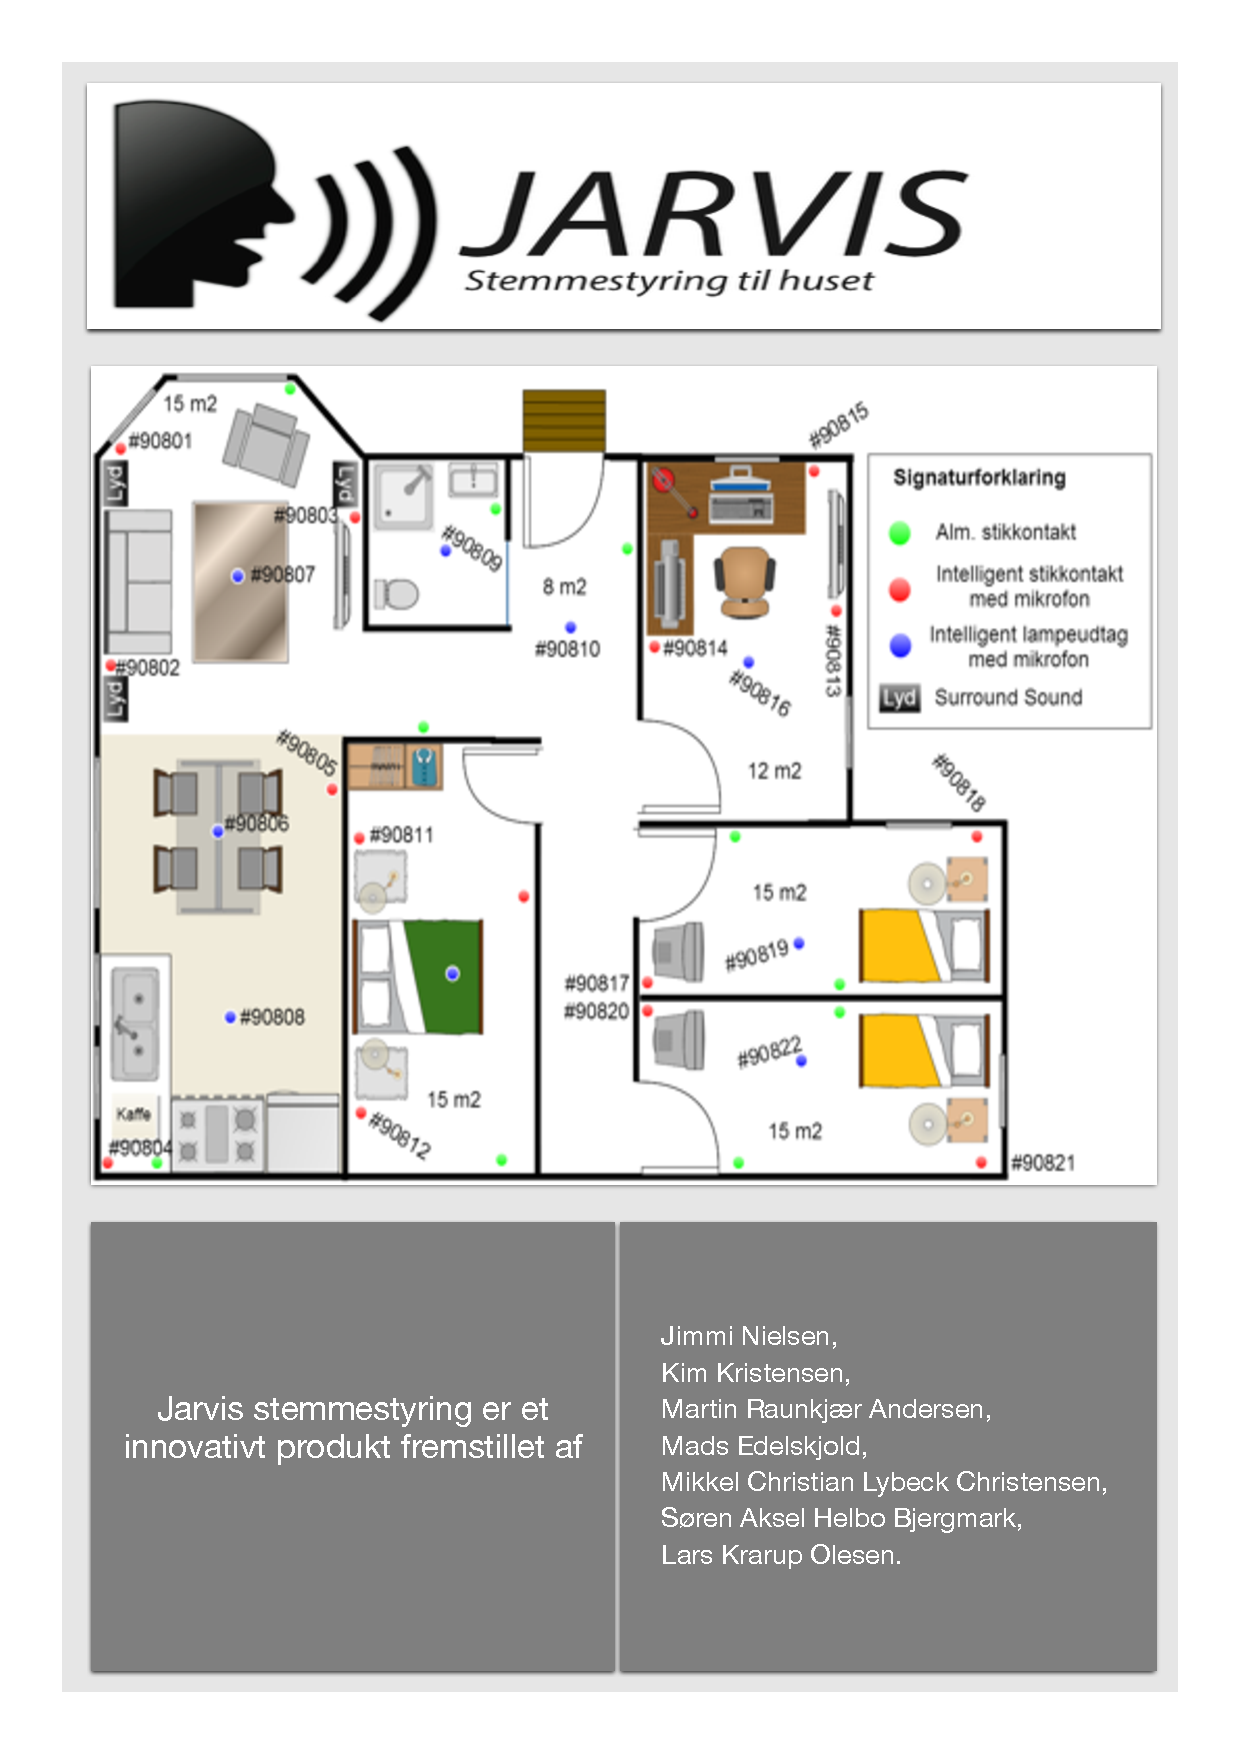
\includepdf{forside.pdf}

\begin{titlepage}
    \setlength{\textwidth}{15cm}
	\noindent
	\begin{nopagebreak}
	{\samepage 
			\begin{tabular}{lr}
				\parbox{0.5\textwidth}{\raisebox{11mm}
					{
\includegraphics[height=3.0cm]{Figurer/Billeder/aauLogo.jpg}}
				} &
				\parbox{0.5\textwidth}{
					\small
					\begin{tabular}{l}
						{\sf\small \textbf{Det Teknisk-Naturvidenskabelige Fakultet }}\\
						{\sf\small  \textbf{Software - 1. studieår}} \\
						{\sf\small Strandvejen 12-14} \\
						{\sf\small Telefon 96 35 97 31} \\
						{\sf\small Fax 98 13 63 93} \\
						{\sf\small http://tnb.aau.dk}
					\end{tabular}
				}
			\end{tabular}
			
			\noindent
			\begin{tabular}{cc}
				\parbox{7cm}{
					\begin{description}
			
						\item {\bf Titel:} 
			
							\textbf{\rapportnavn}\\
							
			  
						\item {\bf Tema:}

							Fra eksisterende software til modeller
			
						\item {\bf Projektperiode:}\\
			  				P1, 08-10-2013 - 18-12-2013 
			 				\hspace{4cm}
						\item {\bf Projektgruppe:}\\
							B2-24
			  				\hspace{4cm}
						\item {\bf Deltagere:}\\
							Jimmi Nielsen\\
							Søren Aksel Helbo Bjergmark\\
							Martin Raunkjær Andersen\\
							Mikkel Christian Lybeck\\
							Kim Kristensen\\
							Lars Krarup Olesen\\
							Mads Edelskjold
							\hspace{2cm}
						\item {\bf Vejledere:}\\
							Jane Billestrup - Hovedvejleder\\
							Morten Bidstrup - Bivejleder

						\item {\bf Oplagstal:} 9
						\item {\bf Sidetal:} \numpages
						\item {\bf Appendiks:} 4
						\item {\bf Bilagsantal og art:} 3x papir, 1x CD
						\item {\bf Afsluttet den:} 18-12-2013
					\end{description}
					\vfill
				} &
				\parbox{7cm}{
					\vspace{.15cm}
					\hfill 
					\begin{tabular}{l}
						{\bf Synopsis:}\bigskip \\
						\fbox{
							\parbox{6.5cm}{\smallskip
								{\vfill{\small %Skrevet af Jimmi
%Sidst rettet: 09-12-2013, 19:56, Jimmi
Denne rapport omhandler automatisering af hjemmet. De nuværende automatiseringsløsninger er blevet optimeret i årevis, hvorved brugerne har opnået økonomiske besparelser, øget sikkerheden samt større fleksibilitet i hverdagen. Alt interaktion med det automatiske systemet har desværre den svaghed, at det kræver brugerens input, i form af smartphone, tablet eller computer, for at den ønskede handling kan blive udført. Disse problemstillinger tager rapporten udgangspunkt i ved at konstruere en stemmestyret softwareløsning, som kan anvende stemmestyring i samspil med det eksisterende system. Herved kan de ønskede handlinger foretages af brugeren, ved at anvende stemmen som input, på en hurtigere og effektiviseret måde.
								\smallskip}}
							}
						}
  					\end{tabular}
  				}
			\end{tabular}
		}\\
		\\
	\noindent{\footnotesize\emph{Rapportens indhold er frit tilgængeligt, men offentliggørelse (med kildeangivelse) må kun ske efter aftale med forfatterne.}}
	\end{nopagebreak}
\end{titlepage}
\clearpage
\newcommand{\doublesignature}[2]{
    \parbox{\textwidth}{
        \vspace{1.5cm}
        \parbox{.48\linewidth}{
            \centering
            \rule{\linewidth}{.7pt}\\
            #1 
        }
        \hfill
        \parbox{.48\linewidth}{
            \centering
            \rule{\linewidth}{.7pt}\\
            #2
        }
    }
}
\newcommand{\singlesignature}[1]{%
    \parbox{\textwidth}{
        \vspace{1.5cm}
        \parbox{.48\linewidth}{
            \centering
            \rule{\linewidth}{.7pt}\\
            #1 
        }
        \hfill
    }
}

\noindent{\doublesignature{Kim Kristensen}{Martin Raunkjær Andersen}}\\\\\\\\
\doublesignature{Søren Aksel Helbo Bjergmark}{Mads Edelskjold}\\\\\\\\
\doublesignature{Jimmi Nielsen}{Lars Krarup Olesen}\\\\\\\\
\singlesignature{Mikkel Christian Lybeck Christensen}
\clearpage

\section*{Forord}
%Skrevet af Jimmi.
%Sidst rettet: 07-12-2013, 17:57, Jimmi
Denne rapport er udarbejdet af en gruppe software-studerende på 1. semester ved Det Teknisk-Naturvidenskabelig Fakultet på Aalborg Universitet. \\\\
I projektet har gruppen taget udgangspunkt i AAU-modellen, som omhandler problembaseret læring.
AAU-modellen tager afsæt i problemorienteret projekt- og gruppeorganiseret læring, hvilket grundlæggende består i en læringsproces, der indledes med en problemanalyse. Denne analyse danner herefter grundlag for rapportens videre bearbejdning af problemets løsning eller forbedring. \\\\
Gruppen vil indledningsvis sige tak til gruppens hovedvejleder, Jane Billestrup og gruppens bivejleder, Morten Bidstrup for deres vejledning – som grundlæggende har dannet rammerne for rapportens udførelse, indhold samt tidsmæssige fastsættelse. \\

(Aalborg Universitet, Software, Civilingeniør. 2013)

\subsection*{Læsevejledning}
%Læsevejledning% %Jimmi og Martin%
%Sidst rettet: 15-12-2013, 17:57, Jimmi
{\bf Komposition} \\
Rapporten er kompositorisk opsat således at overemnet: ”Automatisér dit hjem” indledes som et vidtstærkt og udefinerbart begreb, hvilket gruppen indledningsvis ønsker at begrebsliggøre. I problemanalysen vil gruppen løbende foretage kritiske valg, som vil munde ud i en konkretiseret problemformulering. Denne problemformulering vil rekapitulere en konkret problemstilling, som rapporten vil tage udgangspunkt i det efterfølgende kapitel: Problemløsning. \\

{\bf Kilde henvisning} \\
Som kilde henvisninger anvendes Vanvouver-metoden. Dette bliver brugt ud fra hvert afsnit eller citat, som henviser til en specifik kilde i litteraturlisten vil der stå et tal indkapslet. \\
\textit{Eksempel: Påstand/citat\emph{[1]}}.\\

Hvis der i et afsnit er anvendt store mængder information fra en kilde, står kilden efter punktummet i afslutningen af afsnittet.\\
\textit{Eksempel: Afsnit.\emph{[1]}}\\

Litteraturlisten er kompositorisk opsat således, at kilderne er placeret efter den numeriske orden de er anvendt i teksten. Ud fra deres repræsentative nummerering er alle relevante informationer associeret. \\
\textit{Eksempel: Forfatter(e), Titel på artikel/afsnit, sider med relevant information, bogens titel, redaktør, forlagets hjemsted, forlag, udgivelses årstal.} \\

Hvis nogle af informationerne mangler, som f.eks. forfatterens navn, udelades disse informationer i kildebeskrivelsen. \clearpage

{\bf Figur henvisning} \\
I rapporten vil der løbende blive refereret til figurer eller illustrationer. I den kontekstuelle sammenhæng, hvor figurerne anvendes, vil dette være angivet på følgende måde: \textit{[Afsnit.nummer]} \\

\textit{Eksempel: 2. figur i 3. afsnit vil være angivet med følgende referencenummer: [3.2]}. \\

Under figuren vil figurenes referencenummer samt en dertilhørende figurbeskrivelse, som forklarer figurens relevans være påført den pågældende figur. \\ 
\textit{Eksempel: "Erklæring som en figur er kildemateriale til"}. Se figur \ref{fig:FigurEksempel}.\\
\figurw{Figurer/Figureksempel.png}{Eksempel på figur beskrivelse.}{FigurEksempel}{0.3}
%\figurw{Figurer/Sporgeskema/PrioBespar.png}{Hvor højt økonomisk besparelse prioriteres ved stemmestyring af hjem.}{priobespar}{1}
{\bf Fodnote henvisning}\\
Fodnoter benyttes til at inkludere yderligere informationer om et specifikt begreb, \textit{fagudtryk} eller forkortelse. Fodnoterne beskriver sjældent vitale informationer for forståelsen af det omtalte. En fodnote ses ved et lille tal som henviser til sit modstykke i bunden af siden, hvor den vedhæftede tekst er vist. \\

\textit{Eksempel: Fodnote\footnote{Eksempel på fodnote}}.\\

Første gang et specielt fagudtryk eller begreb bliver benyttet, introduceres det enten i en fodnote eller i den kontekstuelle sammenhæng. \\

{\bf Meta-tekst}\\
Hvert afsnit indledes med en meta-tekst som er anført i kursiv. \\

\textit{Eksempel: Dette afsnit indeholder...}. \\

{\bf Tabeller}\\
Løbende vil der blive fremvist tabeller, som vil blive anvendt konstruktivt i konteksten. Disse tabeller anvendes for at give læseren en bedre visualisering af tekstens indhold.

\begin{table}[h]
    \centering
    \begin{tabular}{ l | l }
        Overskrift & Overskrift \\
        \hline \hline
        A & B \\
    \end{tabular}
    \caption{\textit{Eksempel på en tabel. \tabelgroup}}
    \label{tab:abc}
\end{table}

{\bf Kodeeksempler}\\
Der vil i problemløsningens-afsnittet løbende blive refereret til kodeeksempler. 

\textit{Eksempel:}
\kodel{Kode/Code_example.c}{Beskrivelsen af den viste kode er placeret her}{Code_example}{1}{5}





\clearpage

\renewcommand*\contentsname{Indholdsfortegnelse}
\tableofcontents
\clearpage

\chapter{Indledning}
%Skrevet af Martin og Jimmi.
%Sidst rettet: 17-11-2013, 12:55, Jimmi
Igennem tiderne har huset været et vigtigt element for menneskets overlevelse. Siden menneskets spæde start – i Afrika for ca. 120.000 år siden\cite{HumanOrigen}, var det ikke livsnødvendigt for mennesket at bygge et ly. Det havde selvfølgelig nogle bemærkelsesværdige fordele; beskyttelsen mod farlige rovdyr og den kolde nattekulde (det var lige op til den seneste istid)\cite{RecentIceages}. Det var ikke livsnødvendigt, som det blev senere, da grupperinger af vores forfædre udvandrede fra Afrika\cite{HumanOrigen}. De mere nordliggende steder på kloden var hårdere ramt af nattekulden, og det var her elementært for menneskets overlevelse, at kunne holde kroppen varm i løbet af natten. Dette var den primære grund til, at huset konstant blev udviklet på.\\

Meget senere, i det gamle Romerrige, blev der gravet brønde, som var tilsluttet akvædukter – dette var en vellevned som primært kun velhavende romere havde råd til. Dette havde en markant fordel, idet at man ikke længere var nødsaget til at gå udenfor, når man skulle hente vand eller på toilettet. Romernes forøgede adgang til vand i hjemmet resulterede i øget sundhed og livskvalitet samt velstanden.\cite{VandRom} \\

Omkring afslutningen af det nittende århundrede, var de dage hvor huset kun tjente ét formål - nemlig overlevelsen fra nattekulden og rovdyr - for længst ovre. Kvaliteten af et hjem blev ikke længere kun afgjort af hvor godt det var isoleret, men også hvor økonomisk besparende, komfortabelt og miljøvenligt det var. Antallet af hverdagsting man kunne udføre i sit hjem var støt stigende, op til en sådan grad, at det var unødvendigt at forlade huset, for andet end at tage på arbejde og hente mad. Dette var hovedsageligt på grund af den teknologiske udvikling, som bragte forskellige hjælpemidler ind i menneskers liv, såsom opvaskemaskinen, vaskemaskinen og ovnen. Disse hjælpemidler repræsenterede en markant tidsbesparelse og komfortforhøjelse. For eksempel, kunne tøjvaskningsprocessen, før vaskemaskinens indtog, tage en hel dags hårdt arbejde\cite{Houseworklate19th}. Elektricitetens indtog forhøjede effektiviteten yderligere og resulterende i at det efterhånden var muligt, at forlade maskinerne mens de gjorde langt størstedelen af arbejdet.\\

%Den eksplosive teknologiske udvikling i nyere tid\cite{Moore'sLaw} bragte en lang række nyskabende systemer og teknologier på banen, heriblandt stemmegenkendelsessystem, Audrey, som kom i året 1952, udviklet af Bell Laboratories. Audrey var to meter høj, ekstrem omkostningsfuld, forbrugte massive mængder strøm og var vanskelig at vedligeholde. Den have den egenskab at kunne modtage enkelte cifre fra "designerede" talere, dvs. mennesker som talte meget klart, konsistent og i en helt speciel frekvens og styrke\cite{BellLabsAudrey}. I de efterfølgende år blev teknologien videreudviklet, og der findes til dato en stribe af velkendte stemmestyringssystemer; som f.eks. Apples Siri, som ikke alene kan modtage alle ord men agere ud fra dem\cite{SiriFeatures}.\\

Hjemmet er stadig under en eksplosiv udvikling. I dag indeholder hjemmet et utal af elektroniske apparater, og i takt med at mennesket ønsker optimering i livets mange forskellige aspekter, ønskes hjemmet ligeledes optimeret. Husejerne har fået øjnene op for fordelene ved et centralt og intelligent styret system, som kan være med til at gøre dagligdagen for den enkelte husejer lettere\cite{ZensehomeKunder}. Automatisering i hjemmet er dog ikke hvermandseje, så noget tyder på; at systemerne stadig rummer vitale fejl og mangler - men hvilke?
%Og hvilke løsninger forøger tidsbesparelsen i det automatiserede hjem?

%I takt med elektricitets indtog omkring det 19. århundrede\cite{Elhistorie}, steg hjemmets teknologiniveau yderligere. Elektriciteten blev ganske vist opdaget tilbage i det 17. århundrede, men det havde ikke en relevans for det almindelige hjem, før Edison fremviste glødepæren i året 1879\cite{Cubus}. Denne opfindelse gjorde det muligt for den enkelte husejer, at hurtigt og på en enkel måde få lys i huset. Glødepærens introduktion ledsagede til en eksplosiv udvikling i elektroniske apparaturer\cite{Moore'sLaw} – hvilket revolutionerede husejernes indgangsvinkel imod et mere komfortabelt og automatiseret hjem\cite{ElektricitetHistorie}. \\
\section{Det automatiserede hjem}
Et automatiseret hjem er et abstrakt begreb, som instinktivt kan fortolkes vidt forskelligt fra person til person. Rapporten ønsker indledningsvis at begrebsliggøre ”et automatiseret hjem”, da termens grundbetydning er essentiel for læserens forståelse af rapporten.\\

\textit{Automation} afledes af ordet \textit{automatik}, hvilket ifølge Den Danske Ordbog beskrives: \textit{”funktion uden menneskelig indgriben; anordning der sørger for dette”} \cite{AutomationORDNET}.\\

Det er her væsentligt at bemærke, at uanset komponent eller apparat, indbefattes deres handlinger som automatiserede, i så fald, at det sker uden menneskelige indgriben. Eksempler på dette kan være berøringssensorer der blot opererer ved at tænde eller slukke lys, eller et automatisk regulerende varmeanlæg. Så længe den enkelte komponent agere uden menneskelige interaktion, kan selve komponenten kategoriseres som automatisk. \\

Automation i hjemmet er blevet et populært gadget, som oftest ses i private nybyggerier (se afsnit \ref{sec:zensehomeinterview}), hvor brugerne ønsker en mere tidsbesparende, effektiv og fleksibel dagligdag. For mange brugere bidrager automationen af hjemmet til færre bekymringer, idet forskellige scenarier og elektriske apparater kan brugerkonfigureres efter egne behov og ønsker. Ligeledes bidrager disse automatiseringsløsninger til økonomiske besparelser, i form af automatisk standby-slukning.

%Rapportens problemanalyse belyser hvorledes de eksisterende automationsløsninger fungere, og om disse teknologier har åbenlyse problemer, eller mangler. Forbrugernes ønske om et automatiseret hjem (Afsnit \ref{sec:Interessant}). For at belyse disse problemstillinger, er det dog nødvendigt at indsamle noget konkret data. 








%Martin 02:02 15-12-2013
\section{Rapportens struktur}
Rapporten indeholder følgende afsnit:
\begin{enumerate}
    \item Problemanalyse: Belyser hvordan eksisterende automatiseringsløsninger virker, og om der er problemer eller mangler i disse. Herunder følgende underafsnit:
    \begin{itemize}
        \item Dataindsamling: Der indsamles information omkring automatiserede hjem, og problemer der måtte være
        \item Teknologianalyse: Viden om teknologi nødvendig for forståelsen af problemstillinger
        \item Interessentanalyse: En undersøgelse af hvilken målgruppe som problemløsningen bør henvende sig til
    \end{itemize}
    \item Problembeskrivelse: Beskrivelse af den valgte problemstilling, på baggrund af problemanalysen.
    \item Problemløsning: Nødvendige dele til konstruktion af et produkt, som kan løse de valgte problemstillinger. Herunder følgende underafsnit:
    \begin{itemize}
        \item Kravspecifikation: Beskriver de specifikke krav til produktet
        \item Teori: Omhandler teorier nødvendige i udviklingen af produktet
        \item Design: Et boligscenarie, som illustrerer en potentiel indsætning af produktet i et hjem
        \item Implementation: Beskrivelse og test af selve produktet
    \end{itemize}
    \item Diskussion: Diskussion af de forskellige valg og afgrænsninger, taget i forbindelse med udarbejdningen af rapporten
    \item Konklusion: En diskussion omkring hvor godt et svar på problemformuleringen produktet repræsenterer
    \item Perspektivering: En diskussion omkring hvordan produktet passer ind i det store billede, samt hvad der kunne udvikles videre på det
\end{enumerate}
\clearpage

%Sidst rettet: 17-11-2013, 13:19, Jimmi
\chapter{Problemanalyse}\label{sec:problemanalyse}%Skrevet af Jimmi.
%Sidst rettet: 17-11-2013, 13:19, Jimmi
\textit{I følgende kapitel fokuseres der på dataindsamling vha. metodiske værktøjer. Dataindsamling er relevant for at opnå øget indsigt i problemernes omfang, dimension samt udstrækning i det automatiserede hjem. Ydermere undersøges de eksisterende automatiseringsløsninger, for at dissekere deres fordele såvel som ulemper. Interessenternes belyses, og deres subjektive interesser tydeliggøres. Denne foranalyse leder afslutningsvis til et konkretiseret problem som ønskes løst.}
\section{Dataindsamling}\label{sec:dataindsamling}%Skrevet af Jimmi.
%Sidst rettet: 18-11-2013, 21:43, Jimmi
\label{sec:dataindsamling-afsnit}
\textit{Dataindsamling er en yderst effektiv arbejdsmetode, som kan anvendes såfremt én eller flere samfundsrelaterede problemstillinger ønskes belyst. Før at dataindsamlingsprocessen kan påbegyndes, bør det overordnede formål stå krystalklart. Dette er vigtigt når det indsamlede data senere skal behandles og analyseres – her bør resultaterne gerne afspejle konkretiserede problemstillinger, forekomster eller andre samfundsrelaterede fænomener. For at lette bearbejdningsprocessen, er der nogle specifikke fremgangsmetoder, som kan anvendes; triangulering, den kvalitative samt den kvantitative metode. De nedenstående arbejdsmetoder anvendes senere til at konstruere et spørgeskemaundersøgelse samt dybdeinterview (Afsnit \ref{sec:sporgeskema-afsnit})}.\\\\
{\bf Metodetriangulering} \\
For at kunne sikre sig et højt empirisk datasæt\footnote{Udgangspunktet for analysen}, blev der anvendt en metodetriangulering, som består af at kombinere flere metoder, for derved at kunne krydsrevidere det indsamlede data. 
Her anvendte gruppen en kvantitativ analysemetode til at belyse eventuelle problemstillinger eller mangler forbundet med automatisering af huset. 
Dette blev gjort i form af en spørgeskemaundersøgelse. Det indsamlede data blev i analysefasen opretholdt med en kvalitativ analyseform; dybdeinterview (\ref{sec:zensehomeinterview}), som blev anvendt til at be- eller afkræfte de kvantitative problemstillinger. 
Metodetriangulering gav en fordybende grundanalysering, som sikrede kvalificeret indsigt i problemernes omfang. Dette dannede et solidt datagrundlag for den videre bearbejdning af rapporten \cite{AnalyseDanmark}. \\

{\bf Den kvalitative metode}\\
\label{sec:kvalitative_metode}
Den kvalitative metode har en lang række fordele, som kan forbedre det planlagte interview eller samtale. Metoden anvendes primært til situationer, hvor konkrete emner eller problemstillinger er uklare, og som ønskes undersøgt i en særlig høj grad. Her kan interaktionen mellem respondenten og intervieweren give mulighed for øget fleksibilitet, så spørgsmålene løbende kan tilpasses efter respondentens svar. Dette føre til en mere dybdegående analyse – som kan være med til afdække manifeste og latente holdninger, såvel som interessante motiver \cite{KommunikationItA}. \\

{\bf Den kvantitative metode}\\
\label{sec:kvantitative_metode}
Den kvantitative metode anvendes i situationer, hvor en konkret tendens ønskes undersøgt. Metoden tager udgangspunkt i mange besvarelser, som ofte opnås igennem et spørgeskema. Det indsamlede data kan segmenteres ud fra nogle overordnede forudsætninger, såsom køn, alder m.v., for derved at kunne anskueliggøre problemet ud fra vidt forskellige samfundslag. Det er dog essentielt, at der er et højt antal besvarelser, for at kunne udlede et konkret samfundsmæssigt problem. Et højt antal besvarelser i spørgeskemaet kan opnås ved at konstruere et professionelt og objektivt spørgeskema, hvor spørgsmålene er udført med stor omhyggelighed \cite{KommunikationItA}. \\
\subsection{Spørgeskema}%Dataindsamling
%Sidst revideret af Mads d. 18 Nov kl.13:42
\label{sec:sporgeskema-afsnit}

Der er blevet udarbejdet et spørgeskema for at fastslå om der er nogle problemer eller mangler indenfor de eksisterende automatiseringsløsninger til huse. Dette data, kan bruges til at belyse potentielle behov, eller ønsker - for derved at kunne udarbejde et konkret forbedringsløsningsforslag til de eksisterende automatiseringsløsninger.\\ 
Før at spørgsmålene til spørgeskemaet konstruerers, er der dog nogle kvantitative spørgsmål, som bør overvejes. Her er opstillet nogle eksempler:

\begin{itemize}
    \item Hvem skal spørgeskemaet henvende sig til?
    \item Hvad er formålet med spørgeskemaet?
    \item Hvordan opstilles spørgsmålene objektivt, for at undgå indirekte påvirkning af respondentens svar?
    \item Hvordan kan spørgsmålene formuleres og opstilles mest hensigtsmæssigt, for at undgå fejlkilder? 
\end{itemize}
    
Disse ovenstående eksempler, vil blive uddybet nærmere i afsnit \ref{sec:undersoegelsesdesign}.

\subsubsection{Population og distributering}
For at de førnævnte kvantitative metoder (Afsnit \ref{sec:sporgeskema-afsnit}) kan anvendes, er det vigtigt, at få et højt antal besvarelser. Til dette blev gruppemedlemmernes personlige Facebook-konto anvendt som distributionsmedie. \\

I henhold til spørgeskemaets formål, var det vigtigt, at spørgeskemaet rammede respondenter, som allerede ejede et automatiseret system. For at dette kunne lade sig gøre, var det essentielt at spørgeskemaet blev publiceret igennem andre medier, end blot Facebook. Dette skyldes, at gruppemedlemmernes Facebook-vennekreds, har en alder, som formentlig ikke ejer en automatiseret bolig. \\

For at ramme dette segment, blev spørgeskemaet distribueret igennem relevante teknologifora som livingsmart.dk, hifi4all.dk, eksperten.dk samt andre relevante hobbyforumer. Ved at anvende disse medier opnåede gruppen 272 komplette besvarelser, mens der blev registreret 40 ufuldendte besvarelser.
\subsubsection{Undersøgelsesdesign} 
\label{sec:undersoegelsesdesign}
Spørgeskemaet (Bilag \ref{sec:sporgeskema}) er som udgangspunkt udarbejdet med henblik på at opstille korte og præcise spørgsmål. For at realisere dette, er det vigtigt, at spørgsmålene bliver konstrueret således, at respondenten hurtigt kan tage stilling til de angivne valgmuligheder. Ved at opstille Ja/Nej, såvel som simple punkt-spørgsmål, opnås dette mest hensigtsmæssigt. Spørgeskemaet er desuden konstrueret ved hjælp af SurveyExact.\\

På baggrund af, hvad den pågældende respondent besvarer i sine valgmuligheder, vil de næstkommende spørgsmål være tilpasset efter respondentens forrige besvarelser. Denne funktion kaldes Aktiverings-regel\footnote{Anvendes i analyseværktøjet: SurveyXact}. Spørgeskemaet har 9 aktiveringsregler. Dette er for at konstruere et spørgeskema, som både har relevans for respondenter med et automatiseret hjem, men ligeledes for dem som ikke har. Denne funktion er både til glæde for respondenten, men også for at forebygge fejlkilder, som et spørgeskema, uden disse aktiveringsregler, kunne ledsage til. \\

I 6 ud af 22 spørgsmål, er spørgeskemaet udbygget med en ”Andet”-valgmulighed. Dette er for at forebygge eventuelle fejlbesvarelser, som kunne være ledsaget af, at respondenten ikke har den korrekte valgmulighed til rådighed, og derved vælger den tilnærmelsesvise mulighed. \\

Der er anvendt en kvantitativ metode til at undersøge simple parametre som alder, køn o. lign. i form af 19 spørgsmål, der er målbare statistiske. \\

Flere af spørgsmålene er såkaldte udspecificerende spørgsmål, hvilket er den kvalitative metodeform. Disse spørgsmål har til formål, at få et indblik i, hvilke krav respondenterne har til et automatiseret hjem, uanset om de ejer ét eller ej. Ydermere har disse spørgsmål til formål, at få et samlet indblik i nogle af de funktioner, som respondenterne med et automatiset hjem, efterspørger. \\

\subsubsection{Analysering af data}
\label{sec:analysedata}
Ud fra de 272 fulde besvarelser af spørgeskemaet kan følgende tildens ses (Bilag \ref{sec:sporgeskema} for alle resultater og figurer):
\begin{itemize}
    \item Størstedelen af respondenterne er af det mandlige køn (79\%. Figur \ref{spg:kon})
    \item De er relativt unge respondenter. Mellem 18 - 28 år (72\%. Figur \ref{spg:alder})
    \item Studerende på videregående uddannelse (58\%. Figur \ref{spg:beskaftigelse})
    \item Boligen er i gennemsnit tom i 7 - 9 timer (47\%) og 4 - 6 timer (34\%) (Figur \ref{spg:tomtid})
    \item Den gennemsnitlige respondent slukker ikke for standbyapparater (Figur \ref{spg:standbystrom})
    \item De fleste respondenter ville have interesse i et automatiseret hus (78\%. Figur \ref{spg:interesse})
    \item De højest prioriterede funktioner i et automatiseret hjem er
    \begin{itemize}
        \item Automatisk slukning af standbyapparater og automatisk varmestyring
        \item Systemet skal være økonomisk besparende (71\% i høj grad. Figur \ref{spg:prioautosluk}, \ref{spg:priovarmauto} og \ref{spg:priobespar})
    \end{itemize}
\end{itemize}
Ydermere kan det ses på spørgeskemaet, at LKs\footnote{IHC er en automatiserinsløsning udviklet af Lauritz Knudsen} kunder er delvist tilfredse med deres IHC-løsning (Figur \ref{spg:ihcfungerer}) og at Zensehomes\footnote{Automatiseringsproducent. Denne producent uddybes i afsnittet \ref{sec:zensehomeinterview}} kunder er meget tilfredse med deres løsning (Figur \ref{spg:zensehomefungerer}). \\ På grund af Zensehomes gode ry, har gruppen valgt at sætte et eksklusivt interview op med Zensehome, for potentielt at bruge Zensehomes løsning som hardware forudsætning for vores produkt. \\

Spørgeskemaetundersøgelsen viste ydermere, at respondenterne syntes følgende problemer var relevante:
\begin{itemize}
    \item Energispild ved standby strøm
    \item Manglende stemmestyring af automatiserede hjem
\end{itemize}
Disse problemstillinger er meget relevante i forhold til projektet. De vil her blive gennemgået en efter en.\\

{\bf Energispild ved standby strøm} \\
I Figur \ref{spg:standbystrom} kan det ses at kun ca. 50\% af respondenterne afbryder strømmen til elektriske apparater, ved at slukke på stikkontakten når de forlader hjemmet. På figur \ref{fig:priotid} har 71\% af respondenterne (af dem som var interesseret i automatiserede hjem) svaret at de ville prioritere økonomiske besparelser meget højt, hvis de skulle have et automatiseret hjem.\\
\figurw{Figurer/Sporgeskema/PrioBespar.png}{Hvor højt økonomisk besparelse prioriteres ved stemmestyring af hjem. (213 besvarelser med aktiveringsnøgle)}{priobespar}{1}

Energispild er et mangfoldigt emne, som der er lavet et utal af undersøgelser på. Én af disse undersøgelser er foretaget af Vestforsyningen A/S\footnote{Elforsyning lokaliseret i Holstebro}, som har publiceret pjecen ”Gode Elvaner”\cite{GodeElvaner}. Her kan det ses, at flere apparater ikke bliver slukket og derved har unødig standbyforbrug - faktisk op til 400 kWh om året. Dette er blandt andet routere, computere, lys og tv som er de store syndere. Dette kan bekræftes i forhold til gruppens dataindsamling, som viste at ca. 50\% (Figur \ref{spg:standbystrom}) slukker for deres elektroniske apparater. På grund af dette vælger gruppen at kigge videre på Zensehome, som har specieludviklet software der kan eliminere unødig standbyforbrug. \\

{\bf Manglende stemmestyring af automatiserede hjem} \\
Det kan ses på figur (Bilag \ref{fig:priotid}) at 73\% af respondenterne prioriterer tidsbesparelse højt eller meget højt. Det blev foreslået i spørgeskemaet at stemmestyring er en mangel i automatiserede hjem. På figur (Bilag \ref{spg:interesse}) kan det ses at 78\% af respondenterne ville være interesseret i et automatiseret hjem. I afsnit \ref{sec:infosearch} vil der blive undersøgt om denne problemstilling kan løses. \\
\figurw{Figurer/Sporgeskema/PrioTid.png}{Hvor højt tidsbesparelse prioriteres ved stemmestyring af hjem. (213 besvarelser med aktiveringsnøgle)}{priotid}{1}
\subsection{Interview af Zensehome}%Skrevet af Jimmi.
%Sidst rettet: 14-12-2013, 22:00, Jimmi
\label{sec:zensehomeinterview}
Zensehome er én af producenterne af automatiseringscontrollers til det automatiserede hjem, som holder til i Nørresundby. For at høre mere omkring systemet, blev der taget telefonisk kontakt til Zensehome. Zensehome tilbød i denne forbindelse, at gruppen kunne få systemet demonstreret, som gruppen takkede ja til. Formålet ved denne demonstration, var at få en udvidet indsigt i, hvordan et automatiseringssystem fungere - både det rent opsætningsmæssige, såvel som det softwaremæssige. \\

Gruppen forbedredte inden demonstrationen en række kvalitative spørgsmål, som havde til formål, at belyse købsårsager, teknologiske informationer, såvel som bevidste mangler eller fremtidige planer. \\

Disse kvalitative spørgsmål blev opbygget i henhold til Steinar Kvales\cite{BOOK_KVALE}\footnote{Steinar Kvale er leder for Center for Kvalitativ Metodeudvikling sammesteds. Kvale anses som en autoritet inden for kvalitativ forskning.} 7 stadier i en interviewundersøge.
\begin{enumerate}
    \item Tematisering. Her formulerede gruppen indledningsvis en række spørgsmål, som tog udgangspunkt i det, som gruppen ønsker at finde ud af
    \item Design. Her gennemtænkes alle besvarelsesmuligheder, for at undersøge om de er relevante for tematiseringen
    \item Interview. Spørgsmålene blev stillet i en rækkefølge, så de mest relevante spørgsmål blev stillet først. Ydermere var gruppen på forhånd klar over, at demonstrationen ville blive afholdt af en sælger. Sælgerens dybere teknologiske viden blev overvejet, og spørgsmålene blev opstillet, så de var tilpasset til interviewerens kompetenceniveau.
    \item Transskribering og Analyse. Demonstrationen og interviewet nu færdig, og alle besvarelser skulle nu analyseres. Dette betød at det mundtlige materiale, blev finskrevet og kategoriseret.
    \item Verificering. Her diskuterede gruppen, interviewerens pålidelighed og validitet. Det kunne f.eks. være var specifikke problemer forbundet med systemet, som sælgeren bevidst forsøgte at drosle ned, eller bortargumentere.
    \item Rapportering. Sidste stadie er omdannelsen fra det analysebehandlede materiale til en rapportform, hvorved de relevante perspektiver fremføres.
\end{enumerate}

Efter interviewet, kunne gruppen hermed opstille en række fordele og ulemper ved systemet (herunder et udkast) (se hele interviewet i \ref{sec:zensehome_interview}: 
\begin{itemize}
    \item Fordele
    \begin{itemize}
        \item Brugeren slipper for standbystrøm, ved at systemet kan opsættes i tidsintervaller, hvorved elektroniske apparaturer slukkes automatisk
        \item Mulighed for at benytte det gamle el-net under implementationen
        \item Huset kan tilgås uanset enhed og lokation. Køre på internettet, hvorved brugeren kan styre og konfigurere sit system eksternt.
    \end{itemize}
    \item Ulemper
    \begin{itemize}
        \item Systemet kan ikke køre sammen med varmestyringen og alarmsystemet
        \item Prisen er forholdsvis høj (495,- / kontakt)
        \item Elektronisk støj som kan betyde i visse tilfælde, at lyspærer af ukendte mærker - ikke er understøttet
        \item Controllers\footnote{Zensehomes komponenter, såsom stikkontakter, lampeudtag og sensorer} og scenarier\footnote{En konfiguration som afspiller en række handlinger} kan kun afspilles igennem enheder, såsom smartphone, computeren, eller tablet. Dette går ud over det tidsbesparelsen i systemet.
    \end{itemize}
\end{itemize}

Gruppen ønskede ligeledes at finde ud af, hvor stor interesse danskerne har for et automatiseret hjem. Udbredelsen af systemet blev estimeret af Zensehome til at være omkring 1600 - 1700 installationer, primært i private huse. Derudover blev det oplyst at 90 \% af installationerne var i nybyg.\\

Zensehome er specielt relevant i dette projekt, da deres produkt der er let at implementere i gamle huse, idet at enhederne kommunikere over el-nettet (Afsnit \ref{sec:tekzensehome}). Det kan ud fra mødet konkluderes, at tidsbesparelse kunne være ét af elementerne til en problemstilling, som der kunne fokuseres på.

\subsection{Heuristisk evaluering}\label{sec:infosearch}
%Led eventuelt efter flere undersøgelser der kan opretholdes%
I dette afsnit fokuseres der på teknologien stemmestyring. Dette skyldes at gruppen tidligere kunne (afsnit \ref{sec:analysedata}) konkludere, at der kunne være et aktuelt behov for et stemmestyret system i et automatiseret hjem. For at afgøre om stemmestyringsteknologien er udviklet i en sådan grad, at den vil kunne fungere i samspil med eksisterende automatiseringsløsninger, undersøges teknologien yderligere i afsnittet \ref{sec:stemmestyring}. \\

Der findes flere færdigudviklede stemmestyrings-controllere, som kan opfylde brugernes behov for et mere tidsbesparende system (Figur \ref{spg:priotid}). \\
Siri er en udbredt stemmestyringstekonologi, der benyttes i smartphonen iPhone. Apple er producenten af denne smartphone, som er en af de bedstsælgende mobiltelefoner i nyere tid (Europa).\cite{IDCIphone} Apple har indsamlet en fyldestgørende kundetilfreshedsrapport, som kan være relevant i forhold til at dokumentere den generelle kundeoplevelse af stemmestyringsteknologien Siri. Denne undersøgelse viser blandt andet:
\begin{itemize}
    \item 87\% af iPhone 4S brugere benytter sig af Siri mindst en gang om måneden. Af disse er 55\% fuldt tilfredse med Siri og 36\% delvist tilfredse.
    \item 51\% af iPhone brugere siger at det er ekstremt vigtigt, at der er en funktion der minder om Siri på deres næste telefon\cite{SiriUsage}.
\end{itemize}
Ud fra dette kan det konkluderes at stemmestyring er en teknologi, som i samspil med telefoner, har tilfredse brugere. Det kan ydermere konkluderes, at det er en teknologi, som brugerne ser i deres fremtidige elektroniske apparater. På baggrund af denne tilfredshed antages det, at en stemmestyrings implementationen af det automatiserede hjem vil være en populær løsning. 
\subsection{Opsamling}%Skrevet af Jimmi.
%Sidst rettet: 14-12-2013, 23:19, Jimmi
I analysen blev et spørgeskemaet fremstillet, der skulle hjælpe med at belyse respondenternes tildens indenfor automatisering af huse. Foruden dette, kunne der konstateres at der er en generelt stor tilfredshed iblandt brugerne af stemmestyring. Stemmestyring er en teknologi i udvikling, som hele tiden forbedres, hvilket i sidste ende kommer brugerne tilglæde. Spørgeskemaet og den heuristisk evaluering klargjorde at Zensehomes system er velfungerende og brugervenligt.\\ 

Gruppen valgte på trods af denne forundersøgelse, at arbejde videre med Zensehome. Det næste afsnit vil komme nærmere ind på, hvordan Zensehome og stemmestyring fungere.
\section{Teknologianalyse}\label{sec:teknologianalyse}
Ud fra dataindsamlingen som gruppen har udført, kan det ses, at 45/272 af respondenterne har et automatiseret hjem (Figur \ref{spg:automatiseret} og Bilag \ref{sec:bilcd}). Dette leder til spørgsmålet om hvilken producent forbrugeren har. Ud fra det indsamlede data, har de fleste respondenter et IHC system installeret.
IHC (13\% Figur \ref{spg:autprod}). er et produkt udviklet af Lauritz Knudsen, som er et komplet system til hjemmet. IHC styrer røgalarmer, hårde hvidevarer og generel elektronik i hjemmet. Dette system er unikt ved at det inkluderer næsten alt i hele hjemmet, og derved giver forbrugeren en komplet løsning. Den anden højeste med 9\% er Belkin, som producerer mange små dele til at automatisere sit hjem med. Hovedparten af dette ligger indenfor stikkontakter som automatisk slukker ved et bestemt tidspunkt og sensorstyret lamper. (Figur \ref{spg:autprod}). Derimod er der også forbrugere som har Z-Wave (6\%) integreret i deres hjem. Z-Wave er en udenlandsk udgave af IHC (andet firma), med dette menes der, at Z-Wave også inkluderer de fleste ting i hjemmet, men de ting som ikke er gennemarbejdet i IHC - er gennemarbejdet i dette produkt \cite{IHCForum}. Ligeledes lægges der i Z-Wave meget vægt på at hjemmet skal være overvåget fra top til tå. Sidst men ikke mindst ligger Zensehome på 6\%, som udbyder et halvkomplet system til hjemmet. Zensehome integreres i selve el-nettet i hjemmet og derefter kan forbrugeren, selv udbygge hjemmet alt efter hvor meget der ønskes tilsluttet. Zensehome har dog den ulempe, at der ikke kan tilsluttes hårde hvidevarer, hvilket betyder at forbrugeren kun kan tilslutte elektroniske ting med op til 230 volt til systemet. Derimod kan Zensehome overvåge hvor meget strøm apparaterne bruger, og danne grafer for dette.\\\\
%Indledning til emnet%
Gruppen har konkretiseret udvalgt Zensehome og en stemmestyringsfunktion med henblik på at kombinere dem. Zensehome blev valgt da det er en færdig automatiseringsløsning, som henvender sig til den private sektor samt at det er en gennemarbejdet løsning. Stemmestyringen er ligeledes en teknologi, som viste sig at være en teknologi\ref{sec:infosearch}, som forbrugerne var tilfredse med. Afslutningsvis vil der foretages en opsamling, hvor teknologierne sammenholdes.
\subsection{Zensehome}
\label{sec:tekzensehome}
\label{sec:zensehome}
Zensehome er som tidligere nævnt en virksomhed, der har udviklet et produkt til automatisering af huse. Produktet automatiserer en hel del elkomponenter tilsluttet el-nettet.
Systemet hjælper med at formindske strømforbruget, men hjælper også med at gøre tingene i hjemmet lettere for brugeren. \\
Systemet fungerer på den måde, at stikkontakter, lampeudtag udskiftes med Zensehomes kontakter, den såkaldte controller. Derefter bliver disse enheder opkoblet vha. det som Zensehome kalder en PC-boks. Denne pc-boks fungerer ved, at den modtager og sender datapakken til remote-enheder. Remote-enheder kan eksempelvis være lamper, sensorer, EL-gulvvarme og stikkontakter.
\subsubsection{Remote enheder}
Zensehomes systems kan maksimalt håndtere 244 remotes. Denne begrænsning eksisterer, da løsningen kører på en meget langsom overførelseshastighed. Dette medfører, at systemet højest kan sende og modtage til en hvis mængde remotes.
Systemet kører med 2.400 bit i sekundet. Dette er meget langsomt, hvis dette skulle perspektiveres til internettet - eksempelvis computere og lignende.
Firmaet har valgt at bruge denne hastighed ud fra flere tests, som de har foretaget. Testene indebar, at der blev sat en modtager boks op i den ene ende af huset samt en sender i den modsatte ende af huset. 
Derefter udsender sender boksen en række signaler til modtager boksen. Signalerne bliver udsendt i en prædefineret antal og derfor ved test-devicen hvor mange signaler modtager-boksen skal modtage.
Zensehomes testresultater viste, at den største succesrate, kunne opnås ved 2.400 bit/s. Her er der en modtagelsesrate på 93\%, hvilket Zensehome mente at være acceptabelt. Ved interviewet med Zensehome\ref{sec:zensehomeinterview} blev der ligeledes spurgt, hvad der ville ske, hvis de sendte ved 4.800 bit/s. Svaret var, at dette ville resultere i en forringet modtagelsesrate på 63\%. Udover dette nævnte Zensehome at modtagelsesraten ikke blev højere af at sænke overførelseshastigheden til 1.200 bit/s
\subsubsection{Hvordan virker en enhed (remote)} En remote virker ved, at den modtager et input i form af en pakke, som udsendes af kontakten, eller ved at forbrugeren får remoten til at lave et output.  Hvis forbrugeren fra mobil-applikationen eller PC-boksens software vælger at slukke lyset i stuen, vil PC-boksen sende et output, der går ind i den pågældende remote. Derefter venter remoten i maks 2 sekunder på, at den modtager et svar om, at den har udført den handling, som den blev bedt om. Hvis remoten ikke modtager et svar tilbage vil den forsøge at sende datapakken igen.\\ \figurw{Figurer/kontakt.png}{Remote for kontakt \figuregroup}{Remote}{1.0} På Figur (\ref{fig:Remote}) ses en kontakt med fire funktioner og to elektroniske apparater. De to elektroniske apparater er i form af en lampe og en stikkontakt til TV´et, som hver især har 2 funktioner. 
Funktionerne som vist på Figur (\ref{fig:Remote}) kan have forskellige navne (eller ID). Dette betyder at selvom man trykker på kontakt1´s funktion 1, kan den oversætte dette til, at hvis den skal kontakte lampe1 med funktion 2, da dette er den ønskede handling på lampen.
Dette er en form for synonym for, hvad man skal trykke på således at Kontakt1 (Funktion1) ---> Lampe1 (funktion2).
Hvis forbrugeren trykker på kontakten (kontakt 1 med et kort tryk) ville den sende et signal til den elektroniske genstand, som i dette tilfælde ville være lampe 1 svarende til funktion 1, som illusteret på Figur (\ref{fig:Remote}). Lampe 1 ville derefter modtage signalet og efterfølgende ændre status for hvilke funktioner, som lampen har. Det betyder, at hvis lampen er tændt, vil den slukke og hvis den er slukket, tænder den. Der er dog eksempler på, at den elektroniske genstand har flere funktioner end blot to funktioner, nemlig tænd og sluk. Eksempelvis kan der være funktioner som lysdæmpning, standby slukning og sensorstyring. I dette tilfælde vil kontakten, som forbrugeren trykker på, sende et id samt en funktion med i signalet, som repræsenterer funktionen, som remoten skal gennemføre.\\ Dette betyder, at en kontakt kan have mere end en funktion som vist på Figur (\ref{fig:Remote}), da den måler input på flere forskellige måder. Dette er f.eks. lange og korte tryk, hvor man kan sætte lysdæmpning til et langt tryk (funktion 3 på fig. \ref{fig:RemoteTilLampe}) og korte tryk til at slukke (funktion 1\&2 på Figur (\ref{fig:Remote})). Forbrugeren kan selv vælge en handling, som kontakten skal udføre, når den opfanger et langt eller kort tryk. Et scenarie kunne eksempelvis opstilles på den måde, at en bruger ønsker, at foretage et kort tryk på kontakten for at tænde lampen. Herefter kunne brugeren have behov for at dæmpe lyset, hvilket så bliver gjort ved et langt tryk på samme knap. \figurw{Figurer/remotetillampe.png}{Remote (kontakt) til lampe \figuregroup}{RemoteTilLampe}{0.5} På Figur (\ref{fig:RemoteTilLampe}) ses det, at forbrugeren trykker på en knap på kontakten, som derefter sender et signal til lampen. Dette signal indeholder et id. Signalet modtages så af lampen, som derefter ser efter, hvilket id som blev sendt til lampen. Herefter udføres den valgte handling.
For at give et overblik over systemet har hver en handling et id, som gør, at der kan tilknyttes flere enheder og handlinger til en kontakt. Dette giver mulighed for at have en funktion til at slukke alt, hvad der ønskes i hele huset på en gang. Funktionen sluk alt fungerer via. broadcast\footnote{Udsending af datapakker, til flere enheder på en gang}, hvor man har en enhed i form af en kontakt, som sender et signal til flere elektroniske enheder. Hvis en af enhederne fejler, vil denne genstand ikke slukkes, da genstanden ved broadcast ikke har en sikkerhed for, at signalet bliver modtaget i enheden. \\

Den grafiske illustration af dette, ville se således ud:

\figurw{Figurer/flereremotes.png}{Fra 2 remotes til flere komponenter \figuregroup}{flereremotes}{1.0} 

\subsubsection{Zensehome App}
Det er muligt at tilslutte en installation af Zensehome til internettet, hvis man tilkøber en PC-boks med netmodul. Modulet har en app, som fungerer både på styresystemet Android og iPhones iOS-styrestem. Dette giver forbrugeren mulighed for, at kunne styre et system, selvom brugeren ikke er til stede fysisk. Dette gøres enten via TCP protokollen, der kan sikre, at pakken bliver modtaget eller af UDP protokollen, som ikke har nogen sikkerhed på, at pakken bliver modtaget. UDP protokollen er nyttigt i broadcast, da den dermed ikke skal kontrollere, at signalet blev succesfuldt modtaget, hvilket øger hastigheden. Signalet modtager applikationen via routeren, som skal lukke dataen ud gennem det interne net i hjemmet. For at forbrugeren kan tilgå systemet via applikationen fra internettet, skal systemet have adgang til internettet. Dette kræver dog, at routeren er sat op til portforwarde, da det normalt ikke er tilladt, at udefrakommende kan kommunikere med systemet.

\figurw{Figurer/app.png}{Pakkers vej igennem systemet via APP/PC-Boks \figuregroup}{app}{0.7}
På Figur (\ref{fig:app}) ses en trådløs router, som har 3 elektroniske komponenter forbundet. Ikke alle disse genstande kan tilgås fra internettet - derfor bruger man port forwarding. Portforwarding giver pakkerne direktioner til, hvordan pakkerne skal komme igennem netværket. Dette er illustreret på Figur (\ref{fig:app}), der viser, hvordan en pakke får forbindelse til den rigtige "computer/elektronik udstyr".\\ PC-boksen kører over port 10001. Dette er dermed standardporten, som PC-boksen kan kontaktes på. Hvis det ønskes, kan brugeren ændre dette for at forøge sikkerheden. Dermed opsættes routeren til at sende alt data, som kommer ind på port 10001 videre til PC-boksen, som vist på figur (\ref{fig:app}). Denne konfiguration gør systemet let tilgængeligt, men også mere usikkert på nogle områder da det giver endnu en indgang til systemet udefra, som kan misbruges.
\subsection{Stemmestyring}
\label{sec:stemmestyring}
Stemmestyrings-controllere er en yderst kompleks teknologi, der første gang blev fremvist af Alexander Graham Bell i året 1870. Alexander G. Bell opdagede en sammenhæng i vores sprog, og hvordan ord og sætninger kunne opdeles i fonemer\footnote{fonem: \textit{Den mindste udtaleenhed i et sprog som ved ombytning med en anden, fungerer betydningsadskillende}\cite{DDOfonem}}. Han ønskede en enhed, der kunne transformere nogle få sætninger til et billede, som han kunne bruge til hans hørehæmmede kone. Paradoksalt nok førte denne idé i stedet til telefonen\cite{SpeechGUIDE}. Sidenhen er der sket meget på området af stemmestyrede controllere. Bell Laboratories og IBM videreudvikledte i året 1950-1960 konceptet om én controller der kunne omsætte analoge stemmer til digitale impulser. I 1970’erne videreudviklede ARPA Speech Understanding Research systemet, hvor de i højere grad fokuserede på problemstillingen; at forstå sætningen, fremfor at identificere sætningen – hvilket var en anderledes og ny vinkel at anskue anordningen fra. I dag anvendes stemmestyring i de fleste smartphones; herunder Android, iOS samt Windows Phone. Styresystemerne anvender stemmestyring som en integreret del, hvorved man kan foretage forskellige handlinger, såsom åbne at applikationer, tale-til-tekst, sætte alarmer samt navigationen uden brug af tastaturet. I takt med at stemmestyring er blevet mere alment tilgængeligt, er det nu også en integreret softwaredel i fjernsyn\cite{SpeechSamsung}, hvor brugeren har mulighed for at tænde, slukke samt skifte kanaler vha. stemmestyring. Det bedste og mest udviklede software indenfor stemmestyring er Dragon, som er en videreudvikling af IBM og Bell Laboratories' teknologi, og dermed den teknologi som har haft flest år på banen.\cite{SpeechMIT} I takt med at teknologien blomster, og elektroniske apparaturer bliver mere og mere avanceret, er der ligeledes sket en mærkværdig udvikling på stemmestyrings området. 

\subsubsection{Teknologisk gennemgang}
Stemmestyrings-controllere har flere intrikate\footnote{intrikate: \textit{indviklet; vanskelig at løse ofte pga. pinagtige omstændigheder}\cite{DDOintrikate}} trin der skal gennemføres, før at inputtet, altså stemmen, kan fortolkes af controlleren, og føre til en handling. Første og fremmest indsamles der digitale stikprøver, der måler på stemmens vibrationer, hvilket måles henover regulære tidsintervaller. En analog-digital konverter omsætter sproget til binær kode, som computeren kan forstå (figur \ref{fig:Analog}). Herefter analyseres den binære kode for uønsket støj, kategoriserer frekvenserne samt normaliserer lydhastigheden – hvilket er relevant, da mennesker snakker i vidt forskellige niveauer og hastigheder. Herefter splittes inputtet i 100-1000 dele af sekunder (afhængig af den pågældende controller). Det splittede input analyseres nu yderligere, hvor der undersøges for konsonanternes lyde som ’p’ og ’t’, hvilket sammenlignes med sprogets fonemer. Afslutningsvis konfereres fonemerne i en kontekstuel sammenhæng, hvor dataene gennemløbes i en kompleks statistisk model, som kigger på eksisterende ord, talemåder og sætninger. Med dette gennemløb af handlinger, dechifreres\footnote{dechifreres: \textit{analysere og forstå}\cite{DDOdechifrere}} brugerens input og hvis talen blev tydet korrekt, oversættes det til skrift, handling eller måske noget helt tredje\cite{SpeechMIT}.\\\\
\figur{Figurer/speech-recognition-sample.png}{Her ses en sammenhæng mellem stikprøvens præcision, altså inputtet, og den samlede kvalitet af outputtet \cite{SpeechHowStuffWorks}}{Analog}

\subsubsection{Problematikker forbundet med stemmestyring}
\label{sec:problemer_med_stemmestyring}
Der er flere problematikker forbundet med stemmestyrings-controllere; baggrundsstøj er en notabel fejlmargin, som kan betyde at inputtet ikke forstås korrekt og dermed foretages den ønskede handling ikke. I situationer hvor flere stemmer overlapper hinanden, som til møder, vil stemme-controlleren ikke filtrere inputtet – dette er også problematisk idet de mange stemmer alle skal analyseres og segmenteres, hvilket kræver meget processorkraft.\\
Sætninger, ord og dialekter kan alle være syndere til, at stemmestyringscontrollere ikke kan forstå inputtet. Flere ord staves og udtales ens, men bruges forskelligt i forhold til sammenhængen de er sagt i. Desto større databaser stemmestyringscontrolleren skal lede i, desto mere præcis vil resultatet også være. Databaserne udvides hele tiden, og controllerne har derved en markant højere sandsynlighed for at forstå inputtet korrekt, end hvad der var tilfældet for blot et par år tilbage \cite{SpeechMIT}\cite{SpeechHowStuffWorks}.
\subsection{Opsamling}
Zensehomes automatiseringløsning er et system, der opfylder den private forbrugernes mest centrale behov. Det er dog helt elementært at bemærke, at på trods af at teknologien er så udviklet, foretager det automatiserede system først handlinger i et scenarie-programmeret mønster. Ønskes disse scenarier – altså en række forprogrammeret handlinger afspillet, kræver det at brugeren tager telefonen op af lommen, går ind på applikationen, for herefter at bevæge sig ind på det ønskede scenarie. Dette tager relativt lang tid, og en ulempe i forhold til at systemet skal være lettilgængeligt og tidsbesparende. Denne proces kunne gøres lettere ved at kombinere stemmestyrings-controlleren fra Dragon i Zensehomes komplette system.
\section{Interessenter}%Skrevet af Mikkel og Kim.
%Sidst rettet: 15-12-2013, 18:50, Jimmi
\label{sec:Interessant}
I dette afsnit undersøges de forskellige interessenter. Deres subjektive påvirkninger analyseres, for at belyse de positive, såvel som de negative følger af et stemmestyret system. Interessenterne undersøges med fokus på hverdagen, hvoraf de rutineprægede hverdagsopgaver fremføres. Interessenternes påvirkninger vil ene og alene blive set fra den indgangsvinkel, at de allerede har et automatiseret system installeret. Det betyder, at interessenternes påvirkninger vil blive set uafhængigt af nuværende automatiseringssystem, men ene og alene ud fra et supplerende perspektiv, som et stemmestyret system kunne bidrage til. \\

Hver interessent vil blive gennemgået hver for sig, som afslutningsvis vil munde ud i et afgrænsningsafsnit, som vil samle, og opretholde interessenternes påvirkninger.

\section{Gennemsnitsfamilien} 
For den gennemsnitlige danske familie, vil et stemmestyringssystem kunne bidrage til en mere effektiv såvel som komfortabel hverdag. De tidsbesparende elementer kunne her være, at samtlige controllere, scenarier og konfigurationer kan foretages vha. simple stemme-kommandoer. Et praktisk anvendelseseksempel kunne være konsekvente handlinger, såsom at slukke alt lyset i stuen, i gangen og fjernsynet, blot ved at sige en simpel kommando. Under aftensmaden vil forældrene hurtigt kunne foretage en kontrol, om hvorvidt børnene har husket at slukke lyset på deres værelser. Dette ledsager ligeledes til øget komfortabilitet, idet at brugerne vil kun foretage handlinger, uden at skulle foretage fysiske bevægelser. Et praktisk eksempel kunne her være, at brugeren har 3 lamper i stuen, som ønskes slukket i forbindelse med film-aften. Her kunne brugerne – i stedet for at rejse sig, og slukke dem manuelt – blot sige en kommando, for at udføre en sluk-handling. \\

Et stemmestyringssystem vil dog ikke kun have positive følger. De negative påvirkninger kunne være, at den enkelte familie, opstiller en række scenarier, som går ud over det sociale sammenværd. Dette kunne eksempelvis gå ud over børnene, som måske tidligere er blev lagt i seng sammen med godnatlæsning af forældrene. Her kunne stemmestyring lede til, at forældrene blot anvender en kommando, som slukker alt elektronisk apparatur på børneværelserne, for at indikere at det er sengetid. Foruden dette kunne stemmestyringssystemet lede til et Big Brother-kontrollerende hjem, hvor forældrene hurtigt kan få en statusopdatering på børnenes tændte apparaturer, for derved at undersøge om børnene overholder sengetiderne.
De førnævnte eksempler er blot en bestanddel af praktiske anvendelsesmuligheder stemmestyring kan bidrage til.

\section{Handicappede og ældre} 
Et andet segment i forhold til de private brugere, er de ældre og de handicappede. For dem ville et sådant system ikke kun øge komforten, men især livskvaliteten. Systemet vil være at betragte som et hjælpemiddel, der hjælper til øget funktionalitet i dagligdagen.\\Et eksempel kunne være at kørestolbrugere vil kunne bede systemet om at åbne døren, så det bliver nemmere at komme rundt i hjemmet.\\
I forhold til de ældre, vil systemet også kunne klare nogle af deres besværligheder i hverdagen - dette kan dog have nogle negative følger. Stemmestyringens kommandoer kræver at brugeren kan huske kommandoerne, hvilket kan være problematisk for den ældre. \\ 
Lægges der i stedet vægt på ét stemmestyringssystem i hjemmeplejen, er der ligeledes både positive og negative påvirkninger. På sigt vil det føre til økonomiske besparelser, idet at borgerne kan foretage flere handlinger på egen hånd, og derved vil plejehjemmet kunne spare personale. Fokuseres der på borgerne, vil dette betyde mindre socialt samvær i forhold til en hjemmehjælper, som det sås da robotstøvsugeren kom ud i hjemmeplejen \cite{robotstovsuger}.

\section{Virksomheder}
Effektivisering er altid i fokus på erhvervsdrevne virksomheder, hvorved en stemmestyret løsning kunne bevirke til øget produktivitet. Et praktisk eksempel kunne være lagerstyring, som ofte kræver konstant ajourføring på opmagasinering. Herforuden ville systemet kunne bidrage til en lang række forbedringer, såsom at informere brugeren, om hvor specifikke vare er lokaliseret fysisk på lageret. Dette er et tidsbesparende element, som ville lede til øget effektivitet, idet at medarbejderne ikke længere skal bruge tiden forgæves på at finde de ønskede varer. Et firma ved navn "Millarco"\cite{Int-virksomheder} har fået en stemmestyringsløsning implementeret, som øger deres effektivitet på lageret. Her benytter de stemmestyringssystemet til blandt andet, at få en lagerstatus samt varebestillinger. Det negative kunne være, at stemmestyringsløsningen automatiserer flere processer, som før i tiden krævede en ekstra medarbejder. På denne måde kan systemet bivirke til fyringer. \\

For virksomheder er sikkerhed alfaomega. Server-rum og andre aflåste lokaler vil kunne tilgås ved stemmemanipulation, hvorved medarbejdere eller andre udefrakommende personer kan tilgå følsomme oplysninger. Ydermere vil system-shutdowns, lede til massive produktivitetstab, afhængig af hvordan den enkelte virksomhed har valgt at sikre sig. 

\section{Offentlige institutioner} 
Offentlige institutioner som børnehaver, plejehjem og biblioteker vil bruge et stemmestyret system, som supplement til deres daglige gøremål.\\ 

En børnehave vil kunne bruge et stemmestyringssystem til at holde børnene aktive hele dagen. Dette kan lade sig gøre, ved at der bliver udviklet et system som har nogle forskellige aktiviteter, som børnene ville kunne styre med stemmen. Dette kan resultere i at børnene på et tidligt stadie, lære at bruge IT i deres dagligdag. \\

På bibliotekerne ville man kunne bruge systemet til hurtigt at finde de bøger man leder efter. Bibliotekarerne ville ligeledes kunne ajourføre bibliotekernes lager ved brug af stemmen. Dette effektiviserer bibliotekerne i en retning, som både de ansatte kan få glæde af, men også forbrugerne, som hurtigt vil kunne finde deres ønskede materiale. Systemet vil have en række konsekvenser, som at forbrugerne ikke længere vil kunne stille ukonkretiserede spørgsmål, som ikke er inkorporeret i systemet. Dette vil stadig kræve, at bibliotekarer er fysisk tilstede. Systemet vil dog til stadighed – vil kunne løse mange generelle problemstillinger.

\subsection{Afgrænsning af interessenterne}
Efter at have belyst de forskellige, vigtige interessenter ses det, at der er utrolig mange aspekter i et stemmestyret system. Der er blevet fremvist en lang række tidsmæssige besvarelser, såvel som forøget komfort, hvilket er generelt for alle interessenterne. Ydermere kunne der berettes, at stemmestyring har negative følger, som sikkerhedsmæssige aspekter samt formindskende socialt samvær. For at bygge videre på Zensehomes løsning, er der blevet afgrænset til, at fokus skal ligges på gennemsnitsfamilien. Ligeledes ønsker gruppen at se bort fra de sikkerhedsmæssige aspekter, som er stærkt associeret med virksomheder og ældreplejen. Ved den gennemsnitlige familie kunne det desforuden være interessant at kigge videre på forøget tidsbesparelse såvel som komfort. Nedenunder er opstillet de positive og negative påvirkninger den gennemsnitlige familie vil kunne opleve ved et stemmestyret system: 
\begin{itemize}
    \item Positive påvirkninger
    \begin{itemize}
        \item Tidsbesparelse og øget komfort
        \begin{itemize}
            \item Styring af controlleres status - dvs. at tænde og slukke for elektriske apparater
            \item Opsætning, redigering samt sletning af scenarier og controllers
            \item Økonomiske besparelser (hurtig kontrol/ændring af controllers status)
            \item Øge fleksibilitet i hverdagen
        \end{itemize}
    \end{itemize}
    \item Negative påvirkninger
    \begin{itemize}
        \item Formindske det sociale samvær
        \begin{itemize}
            \item Forældrenes kvalitetstid med især børnene kan formindskes
            \item BigBrother-lignende hjem, hvor overvågning tager overhånd
        \end{itemize}
    \end{itemize}
\end{itemize}

Valget af interessenterne er ydermere baseret ud fra resultaterne af spørgeskemaet \ref{sec:sporgeskema-afsnit}, som hovedsageligt henvendte sig til den almindelige dansker. Gennemsnitsfamilien er derfor valgt som interessant.
\clearpage

\chapter{Problembeskrivelse}
\label{sec:problembeskrivelse}
%Skrevet af Jimmi.
%Sidst rettet: 18-11-2013, 21:51, Jimmi
\textit{I følgende kapitel samles hele problemanalysen til et konkret problem, som rapporten fremadrettet vil fokusere på. De samfundsrelaterede problematikker er blevet fremvist – viderebehandlet og analyseret, og vil i det kommende afsnit blive opsummeret. Problemafgrænsnings-afsnittet vil opsamle afgrænsningerne, der blev foretaget tidligere i problemanalysen. Problemformuleringen vil afslutningsvis forbinde problemafgrænsningen og det pågældende løsningsforslag.} 
\section{Problemafgrænsning}
%Skrevet af Jimmi.
%Sidst rettet: 19-11-2013, 16:34, Jimmi
Problemanalysen har belyst konkrete samfundsrelaterede problemstillinger ved det automatiserede hus. Ud over at belyse problemstillingerne forbundet med de eksisterende teknologier, har problemanalysen også givet et solidt udgangspunkt hen imod relevante samfundskritiske problemstillinger. De eksisterende teknologier, er blevet dissekeret; hvor især ulemperne fra teknologierne kan revideres – i håbet om at – i sidste ende, at konstruere en mere raffineret teknologi. \\\\
Dataindsamlingen-afsnittet (Afsnit \ref{sec:dataindsamling-afsnit}) fremhæver særligt de økonomiske besparelser, som kan opnås ved én automatiseringsløsning, men lige så vigtigt, er brugernes ønske om et tidsbesparende system. Nutidens automatiseringsløsninger fokuserer primært på de økonomiske besparelser, simpelthen ved at slukke for de elektroniske apparaturer ved unødig brug. Zensehome’s automatiseringsteknologi blev grundlagt i bestræbelserne på at opnå økonomiske besparelser. Foruden de økonomiske besparelser, blev systemet konstrueret således at systemet kunne implementeres på det gamle el-net. Blev husstanden på et senere tidspunkt udbygget, var det essentielt, at forbrugerne selv kunne tilpasse systemet. \\
I bestræbelserne på at optimere systemet yderligere, blev der på baggrund af dataindsamlingen (Afsnit \ref{sec:dataindsamling-afsnit}), lagt særlig vægt på forbrugernes ønske: tidsbesparelse. Under interviewet (Afsnit \ref{sec:zensehomeinterview}) med automatiseringen-producenten, Zensehome, blev der bemærket, at alt interaktion mellem forbrugeren og huset, skulle foregå via tablets, smartphone eller computer. Ydermere krævede afspilningen af scenarierne, at enheden skulle findes frem – applikationen skulle åbnes – for til sidst at trykke på det ønskede scenarie. Processen kunne være tidskrævende og anstrengende for forbrugeren. På baggrund af respondenternes høje ønsker om et mere tidsbesparende system, konkluderede gruppen, at det er her fokus skulle ligges. I præcis samme boldgade var stemmestyring-controllere, som viste et højt tilfredshedsniveau iblandt forbrugerne. Henholdsvis 55\% og 36\% af Siris kunder viste fuldt tilfredshed, samt delvist tilfredshed (Afsnit \ref{sec:infosearch}). Ydermere kunne det konkluderes, at teknologien havde fået et gennembrud blandt verdens største elektronik-fabrikanter – Samsung, Android-styresystemet samt IPhone (Afsnit \ref{sec:stemmestyring}).

\section{Problemformulering}
%Skrevet af Jimmi.
%Sidst rettet: 19-11-2013, 17:34, Jimmi
Det tidsbesparende aspekt er valgt som fokuspunkt. Der er mange forskellige interessenter, som har interesse i et tidsbesparende system (Afsnit \ref{sec:Interessant}). Den primære målgruppe for produktet er gennemsnitsfamilien, da øget komfort kan forbedres, ved at anvende et tidsbesparende system. De elektroniske apparater kræver i høj grad en interaktion fra brugeren – hvornår de skal tænde, hvornår de skal slukke, og ikke mindst hvornår udstyret skal stå på standby. For mange familier, ligner dagene ikke altid hinanden, og hverdagsmønstreret ændres konstant. Eksisterende teknologier (Afsnit \ref{sec:zensehome}) forsøger at tage højde for problemstillingen, ved at give brugerne mulighed for at tænde og slukke forprogrammerede enheder via. Smartphones, tablets eller computere. Det er dog tidskrævende at først programmere de ønskede scenarier, for derefter at afspille dem. \\\\
Det er vigtigere end nogensinde, at effektivisere sin hverdag hensigtsmæssigt, for derved at undgå tidsspild. Denne effektivisering foregår også i hjemmet, hvor et utal af elektroniske apparaturer kræver menneskelige interaktion. Det kunne hermed være en stor fordel, hvis interaktionen med huset, blot fungerede ved brug af stemmen. Herved opnås den ønskede tidsbesparelse, og derved den ønskede komfort. Ved sene aftentimer, hvor familien ankommer til huset, og blot ved at sige et par ord, forstår huset den ønskede handling – og agere derudfra. Der er et utal af forskellige scenarier, som er nærmest umulig for den enkelte familie at forprogrammere, idet at det daglige mønster - for den enkelte familie - er alt for ustadigt. Det er væsentligt at stemmestyring i hjemmet kan være et supplement til øget komfort, og med det udgangspunkt, ser gruppens problemformulering således ud: 
\begin{itemize}
    \item Hvordan kan to eksisterende teknologier; Zensehome og stemmestyring kombineres med hinanden? \\
    \begin{itemize}
        \item{\bf Hvordan vil det være muligt, at konstruere software til en stemmestyret enhed, som ud fra stemmeinputtet, kan styre elektronisk apparater i husstanden, på en sådan måde, at det giver en tidsbesparelse for den enkelte gennemsnitsfamilie?}
    \end{itemize} 
\end{itemize} 
%Sidst rettet: 13-12-2013, 18:34, Martin
%Sidst rettet: 14-12-2013, 12:34, Jimmi
\hspace*{\fill} \\\\
{\bf Teknisk afgrænsning} \\
Ovenstående problemformulering vil blive lavet i et C-programmeringssprog. Gruppen har ikke fået stillet økonomiske midler til rådighed, som er ensbetydende med, at det endelig produkt blot vil være en simulering, af hvordan det endelige produkt ville fungere. Grundet tidsbegrænsninger (10 ECTS\footnote{European Credit Transfer System}) afgrænser gruppen det endelige produkt til en fungerende simulation af stemmestyring. Hvordan løsningen kan integreres i Zensehome's automatiseringsløsning, er ligeledes noget gruppen har valgt at afgrænse sig fra.




\chapter{Problemløsning}
%Skrevet af Jimmi
%Sidst rettet: 02-12-2013, 16:07, Jimmi
\textit{I følgende kapitel fokuseres der på software-løsningen. Kapitellet indledes med en kravspecifikation, som pointerer de overordnede krav til softwaren. Kravene udbygges herefter med et teori-afsnit, som vil redegøre for de interessante paradigmer, forbundet med stemmestyring. Denne teoritiske viden, vil kunne anvendes i den videre bearbejdningsproces henimod det færdige produkt. Ydermere vil denne teori kunne anvendes til at strukturere en proceshandlings-oversigt, som vil visualisere de overordnede funktionaliteter i programmet. Dette vil lede videre til design-afsnittet, hvor et konkret bolig-scenarie vil være opstillet. Afslutningsvis vil implementerings-afsnittet belyse relevante programdele, som er blevet omsat fra et teoretisk grundlag til en funktionel softwareløsning – her vil et hardwaremæssigt boligscenarie blive opstillet.}


\section{Kravspecifikation}
% Skrevet af Jimmi.
% Sidst rettet: 04-12-2013, 13:35, Jimmi
% Sidst rettet: 10-12-2013, 03:00, Søren
% Sidst rettet: 13-12-2013, 23:18, Martin
% Sidst rettet: 14-12-2013, 11:18, Jimmi
Formålet med kravspecifikation, er at få specificerede entydige krav til programmets kunnen og samlede funktion. Dette er vigtigt, for at programmets samlede funktion, afspejler den samfundsrelateret problemstilling, som ønskes løst. Hvordan og hvorledes programmet bør konstrueres, for at afdække de specificerede produktkrav, vil ligeledes fremgå i det følgende afsnit. På baggrund af problemanalysen (kapitel \ref{sec:problembeskrivelse}), blev der afslutningsvis opstillet en problemformulering. Kravspecifikationens formål, er at skitsere de fundamentale produkt-funktionaliteter, der er påkrævet, for at softwareløsningen vil opfylde den konkrete problemformulering. Denne kravspecifikation er på baggrund af ovenstående, blevet udarbejdet med fokus på følgende: \\

At mindske brugernes tidsforbrug og øge komfortabiliteten under interaktion mellem bruger og system, ved at kombinere Zensehomes system med stemmestyringscontrollere, med henblik på at kunne lette følgende handlingsprocesser:
\begin{itemize}
    \item Øge brugerkomforten ved at gøre det muligt, at alle handlinger kan foretages uafhængigt af rummet brugeren befinder sig i
    \item Mulighed for at oprette, slette og redigere systemets controllere, brugere samt scenarier
    \item Opsætte rettighedssystem, så ikke alle brugere har adgang til det samme
    \item Give tilbagemeldinger ved fejlmeddelelser – såvel som accepterede handlinger, så brugeren ikke er tvivl om den ønskede handling er modtaget som korrekt input
\end{itemize}
\hspace*{\fill} \\
Som nævnt i afsnit \ref{sec:problemer_med_stemmestyring}, er der dog nogle problemer forbundet med stemmestyring. Disse problemer vil gruppen forsøge at løse med følgende funktioner:
\begin{itemize}
    \item Konstruere en stavekontrol-funktion, som vil behandle brugerinputtet, og autokorrigere det til det korrekte
    \item Opstille en tilstandsmaskine, som vil automatisk sætte programmet i forskellige tilstande, afhængig af validering.
\end{itemize}
    
For at overstående kravspecifikation kan realiseres, er der et behov for at dissekere trinene igennem en gennemgang af relevant teori (Afsnit \ref{sec:teori}). Ydermere er der et behov for en systematisk udspecificering af handlingprocessen, og hvornår disse handlinger bør udføres mest hensigtsmæssigt. \\



% Skrevet af Jimmi.
% Sidst rettet: 04-12-2013, 13:35, Jimmi
% Sidst rettet: 10-12-2013, 03:00, Søren
%Formålet med kravspecifikation, er at få specificerede entydige krav til programmets kunnen og samlede funktion. Dette er vigtigt, for at programmets samlede funktion, afspejler den samfundsrelateret problemstilling, som ønskes løst. Hvordan og hvorledes programmet bør konstrueres, for at afdække de specificerede produktkrav, vil ligeledes fremgå i det følgende afsnit. På baggrund af problemanalysen (kapitel \ref{sec:problembeskrivelse}), blev der afslutningsvis opstillet en problemformulering. Kravspecifikationens formål, er at skitsere de fundamentale produkt-funktionaliteter, der er påkrævet, for at softwareløsningen vil opfylde den konkrete problemformulering. Denne kravspecifikation er på baggrund af ovenstående, blevet udarbejdet med følgende fokuspunkter: 

%\begin{enumerate}
%    \item Mindske brugernes tidsforbrug og øge komfortabiliteten under interaktion mellem bruger og system:
%    \begin{itemize}
%        \item Kombinere Zensehome’s system med stemmestyrings%controllere, for derved at kunne lette følgende handlingsprocesser:
%        \begin{itemize}
%            \item Øge brugerkomforten ved at gøre det muligt, at alle handlinger kan foretages uafhængigt af rummet brugeren befinder sig i
%            \item Mulighed for at oprette, slette og redigere systemets controllere, brugere samt scenarier
%            \item Opsætte stemmegenkendelse,\mafix{Det vurderes senere om denne kan nå at blive færdig.} som vil give de forskellige beboere mulighed for at definere forskellige prioriteter og rettigheder
%            \item Give tilbagemeldinger ved fejlmeddelelser – såvel som accepterede handlinger, så brugeren ikke er tvivl om den ønskede handling er accepteret
%            \item Konstruere en funktion, eventuelt i form af en stavekontrol, der vil autokorrigere brugeren ved små stavefejl, spørge brugeren om fundne retteord er korrekt ved størrer stavefejl.
%        \end{itemize}
%    \end{itemize}
%\end{enumerate}

%For at overstående kravspecifikation kan realiseres, er der et behov for at dissekere trinene igennem teoretisk udredelighed (Afsnit \ref{sec:teori}). Ydermere er der et behov for at systematisk udspecificere handlingprocessen, og hvornår disse handlinger bør udføres mest hensigtsmæssigt.

\section{Teori}
\label{sec:teori}
%Skrevet af Jimmi
%Sidst rettet: 07-12-2013, 18:36, Jimmi
I følgende afsnit beskrives nogle af de handlingsprocessor, der skal til, for at stemmestyring kan omdannes fra et analog signal – i form af stemmen, til en programmerbar løsning. Teori-afsnittet er sat op på en måde, således at emnerne forekommer i den kronologisk rækkefølge; indledningsvis ønsker brugeren en kommando udført. Dette input omdannes til en tekststreg, som ledes videre til stavekontrol-afsnittet. Stavekontrollen er essentiel, for at rette eventuelle fejltolkningerne og misforståelser. Afslutningsvis beskriver afsnittet, tilstandsmaskiner, hvordan kontrollen skal foregå kontinuerligt, og i en stadiebaseret helhed.

\subsection{Fra input til handling}
%Skrevet af Jimmi & Mads
%Sidst rettet: 29-11-2013, 16:07, Jimmi
%Sidst rettet: 9-12-2013, 17:14, Mads
Stemmestyrings er en yderst kompleks teknologi, som kræver en lang række operationer, før at inputtet – altså det sagte, kan oversættes til noget som den pågældende controller kan opfange, og videresende til PC-boksen. For at opnå et digitalt og forståeligt datasæt, skal følgende handlinger foretages i kronologisk rækkefølge, som illustreret på nedenstående Figur (\ref{fig:steps_jarvis}).  
\figurw{Figurer/steps_jarvis.png}{Ordet ”Jarvis” er blevet opfanget hos én af huset stemmestyringscontrollere. (Figuren er fremstillet af gruppen, og er blevet konstrueret på baggrund af Pracical Vibrations Analysis \cite{VoiceSteps}}{steps_jarvis}{1}
Stemmestyringsenhederne er blevet navngivet: ”Jarvis”. Dette er et unikt navn, som er assimileret med samtlige controllere i husstanden. Dette er primært for at forhindre systemet i at udføre handlinger, som ikke er målrettet det automatiserede system. Ovenstående Figur (\ref{fig:steps_jarvis}) skal illustrerer hvordan ordet: ”Jarvis” siges af brugeren (input), hvorefter støjende elementer frasorteres, inden konverteringsprocessen påbegyndes. \\\\
Dataen, som den pågældende controller opfanger, vil blive sendt videre til PC-boksen, hvor den videre behandlingsproces vil blive afviklet. Her undersøges der for, om ordet ”Jarvis” er godkendt – i så fald ændres systemet systemets tilstand (\ref{sec:tilstandsmaskine}) til at opfange alle efterkommende ord, idet at systemet nu ved, at brugeren ønsker at foretage en handling. De efterfølgende ord vil gennemgå den samme proces, for at afgøre om hvorvidt der skal sendes en datapakke\footnote{Mere info i afsnit \ref{sec:zensehome}} til det ønskede elektroniske apparat, eller ej. \\\\
Ved at optage og dissekere ordet: ”Jarvis”, kan der fremstilles en grafisk figur. Dette kan lade sig gøre, fordi stemmen består af en lang række forskellige vibrationer og frekvenser. Disse frekvenser kan dissekeres, ved at anvende en forbedret autokorrelations algoritme\footnote{Anvendes til at finde alle tonehøjde afsløringer}. Algoritmen bruges til at få et datasæt, som består af niveau\footnote{Niveauet måles i dB, sm er en enhed for lydstyrke}, frekvens\footnote{Frekvensens måles i Hz. For mere info se \ref{sec:frekvensens_struktur}} og strækning\footnote{Strækningen måles i tid, som afhængigt af datasæt, kan måles ned i tilnærmelsesvise milisekunder} \cite{Autocorrelation}. Idéen med algoritmen, er at fokusere på de fundamentale frekvenser – dette vil sige, at algoritmen fjerner alle negative værdier. Herefter genereres en kopi af optagelsen, hvilket fordobles i strækningstiden. Her anvendes korrektions-algoritmen. Dette gennemløb er for at fjerne alle højdepunkts beskæringer \cite{Autocorrelation}.  \\
Ud fra det genererede data, kan følgende graf fremstilles:
\figurw{Figurer/graph_jarvis.png}{Visualisere inputtet: 'Jarvis', opsat med niveauet som en funktion af tiden. (Figuren er fremstillet af gruppen, og er blevet konstrueret på baggrund af lydprogrammet: Audicity datasæt. jf. algoritmisk værktøj.)}{graf_jarvis}{1}
Figuren viser hvordan ordet ”Jarvis” udgør 6 forskellige spektre\footnote{Frekvensspektret er en målestok-enhed, der bruges til at finde frekvens udstrækning}, som danner rammerne for hvert ord i sætningen. Siges bogstavene separat, men indsættes i det samme tidsmæssige-spektrum, kan der ses en sammenligninghed mellem ordet og bogstaverne – de udgør tilnærmelsesvis det samme antal oktaver\footnote{Intervallet mellem en tonehøjde og en anden med en halv eller dobbelt dens frekvens}! Det der separere de forskellige bogstaver er nul-passage\footnote{Det punkt, hvor der ikke er nogen svingninger til stede}. Dette ses på figuren \ref{fig:graf_jarvis} som når niveauet er 0 \cite{VoiceProject}\footnote{Projektet er udarbejdet af David Wagner, som har en Ph. D. Dartmouth College - Concentration in Computer Science}. \clearpage
Zoomes der ind på ordets begyndelsesbogstav ”J” hvor bogstavet ”J” er sagt separat, kan sammenhængen ses bedre.
\figurw{Figurer/graf_jarvis_j.png}{Visualisere sammenhængen mellem ordet 'Jarvis' og begyndelsesbogstavet 'J'. (Figuren er fremstillet af gruppen, og er blevet konstrueret på baggrund af lydprogrammet: Audacity datasæt. jf. algoritmisk værktøj.)}{graf_jarvis_j}{0.5}
Som det ses på ovenstående figur, kan niveauet være vidt forskellige – til trods for, at der menes det samme. Det er et utal af forskellige parametre der spiller ind, som vil blive yderligere belyst i det kommende afsnit (afsnit 4.2.1.1). 
\clearpage
\subsubsection{Frekvensens struktur}
\label{sec:frekvensens_struktur}
Lydbølger består af en amplitude som afgør lydens niveau. For at afgøre lydbølgers toneleje, måler man på frekvens, som grundlæggende betyder, hvor tit bølgen har lavet en svingning. Figuren viser, hvordan antallet af svingninger er voksende, desto højere frekvenser er. Blå illustrere hvordan bølgelængden ville se ud, hvis svingningstiden var halveret. (Figur \ref{fig:curve_frequency})
\figurw{Figurer/frequency.png}{Illustrerer en svingning, fra bølgetop til bølgetop. (Figuren er fremstillet af gruppen)}{curve_frequency}{1}
Den gennemsnitlige kvinde har en lys og høj grundtonefrekvens på 180-200 Hz, hvor den mandlige stemme til modsætning er dybere, og har en omtrentlig frekvensområde på 100-130 Hz \cite{Stemme}. Dette skyldes stemmelæberne længde og tykkelse. Mænd har de længste og tykkeste, kvindernes er kortere og tyndere mens børns er kortest og tyndest. Det er dog først muligt at analysere på den gennemsnitlige grundtonefrekvens efter 20 års-alderen, idet at stemmelæberne skal være færdigudviklet.\\

Med denne teoretiske viden, vil det være muligt at konstruere systemet, således at antal svingninger over tid, vil være en indikator for den pågældende persons alder. Herved vil det være muligt, at opsætte vidt forskellige prioriteter for husets beboer. \\

Når inputtet er blevet konverteret til en tekststreng, skal tekststrengen kontrolleres for stavefejl, hvilket det næste afsnit (\ref{sec:stavekontrol}) vil komme nærmere ind på.
\clearpage

\subsection{Stavekontrol}
%Skrevet af Martin, Søren og Jimmi.
%Sidst rettet: 03-12-2013, 16:40, Jimmi
\label{sec:stavekontrol}
Stavekontrol i programmeringssammenhæng blev første gang, fremvist af Ralph Gorin i året 1971. Løbende er stavekontrol-faciliteten, blevet en naturlig integration af skriveprogrammer, hvor det anses af de fleste, som værende et uundværligt korrektionsværktøj. \\ Efter Ralph Gorin’s fremvisning, er der løbende kommet forskellige bud på, hvordan teknologien kunne forbedres, specificeres eller tilpasses til forskellige problemstillinger. Stavekontrol er et kæmpe emne i sig selv, og derfor vil der i det kommende afsnit redegøres der for nogle af mest centrale metoder, for at afslutningsvis, kunne fastlægge den mest hensigtsmæssige metode \cite{UnifiedSpellCheck}.\\

For at systemet kan interagere med brugerens stemme, er det helt fundamentalt, at systemet er dynamisk konstrueret. Denne dynamik, vil kunne udmøntes vidt forskelligt, og det derfor essentielt at undersøge de teoretiske principper, for herved at kunne løse den pågældende problemstilling bedst muligt. Når brugeren interagerer med systemet (afsnit 4.2.1), vil konverteringsprocessen være altafgørende for hvordan den færdigkonverterede tekststreng vil se ud. I tilfælde af, at brugeren har snakket utydeligt, skal systemet kunne håndterer dette på en dynamisk og ingeniøs måde. Dette er vigtigt, idet at systemet bør øge brugerens komfortabilitet, og mindske tidsforbruget. \\

\subsubsection{Redigeringsafstand} % Martin & Jimmi. Edit distance.
%Redigeret: Martin 14:46 15-12-2013 
Redigeringsafstandsmetoden virker ved at sammenligne det skrevne ord med en indlæst database – hvorved en lighedsprocent udregnes. Denne lighedsprocent udregnes ved at anvende en algoritme, som tager udgangspunkt i det skrevne ord ($O_1$), og sammenligner med database-ordet ($O_2$). Her måles der på det totale antal bogstavs-indsætninger, sletninger eller erstatninger \cite{UnifiedSpellCheck}. \\\\
Eksempel på redigeringsafstandsmetoden med en redigeringsafstand = 2. \\ $O_1$ : \textit{”Karvise”}, $O_2$ : \textit{”Jarvis”}
\begin{enumerate}
    \item \textit{”Karvise” $\rightarrow$ ”Jarvise”} (Erstatning af K $\rightarrow$ J)
    \item \textit{”Jarvise” $\rightarrow$ ”Jarvis”} (Sletning af e $\rightarrow$ ””)
\end{enumerate}

I ovenstående eksempel udføres redigeringsafstandsmetoden gentagende gange, indtil der er er 100\% sammenligningsgrundlag mellem $O_1$ og $O_2$. Er der flere tilnærmelsesvise ord, vil de fremgå i en prioriteret rækkefølge, med højest lighedsprocent øverst, dvs. de ord med de færreste antal redigeringstrin.

\subsubsection{Lignende nøgler} % Martin & Jimmi. Similarity keys
Lignende-nøgle metoden blev grundlagt, idet at der var flere problemer associeret med fonetiske sætninger; derfor blev en algoritme udviklet, som hurtigt kunne finde de fonetiske fejl. Metoden gik i alt sin enkelthed ud på, at tildele alle ord og udtryk et digitalt signatur, som ikke måtte ødelægge de vigtigste træk i den fonetiske udtalelse af ordet. Der blev foruddefineret en række regler, som bestemte hvorledes konverteringsprocessen fra ord til talværdi skulle foregå \cite{UnifiedSpellCheck}.
\clearpage

Det første bogstav skulle gemmes, og de følgende bogstaver skulle konverteres efter nedenstående digitaliseringsprincipper: \\

\begin{table}[h]
    \centering
    \begin{tabular}{ l | l }
        Digitaliseringkonv. & "Jarvis" \\
        \hline \hline
        A, E, I, O, U, H, W, Y $\rightarrow$ 0. & A, I \\
        \hline
        B, F, P, V $\rightarrow$ 1. & V \\
        \hline 
        C, G, J, K, Q, S, X, Z $\rightarrow$ 2. & S \\
        \hline 
        D, T $\rightarrow$ 3. & \\
        \hline 
        L $\rightarrow$ 4. & \\
        \hline 
        M, N $\rightarrow$ 5. & \\
        \hline 
        R $\rightarrow$ 6. & R \\
        \hline 
    \end{tabular}
    \caption{\textit{Eksempel på lignende-nøgle metoden, med databaseordet: ”Jarvis”. \tabelgroup}}
\end{table}

"Jarvis" ville få tildelt følgende nøgle: J06102. Afslutningsvis elimineres alle 0’erne, og den tildelte nøgle vil derfor blive: J612.

\subsubsection{Regelbaserede sandsynlighedsberegning} % Jimmi & Martin. Rule-based techniques
Regelbaseret stavekorrektions-metoden anvender en algoritme, som beregner sandsynligheden for at ét forkert stavede ord, kan associeres med et eller flere omkringliggende ord. Metoden virker ved at sammenligne det skrevne ord, med en database for derved at kunne kortlægge fejlmønstre. Dette gøres ved at foranliggende såvel som de bagvedliggende ord undersøges i den kontekstuelle sammenhæng. For at kunne returnere det korrekte ord – afhænger denne korrektionsmetode i høj grad af, at databaserne har mange aktive brugere, hvorved gængse fejl og ordsammensætninger kan forefindes. \\\\
Denne metode kunne i stemmestyrings produktsammenhæng anvendes til at lagre brugernes mønstre. Dette kunne være tvetydige udtalelser eller accenter, som systemet løbende ville kunne forebygge, ved at kigge på tidligere korrektioner. Dette er en løsning, som gør brug af elementære sandsynlighedsberegninger, og ville med tiden kunne forebygge en lang række fejlfortolkninger af systemet \cite{UnifiedSpellCheck}. 

\subsubsection{Opsamling}
Stavekontrolsteknologien er som beskrevet i ovenstående kapitel et avanceret værktøj. Metoderne har vidt forskellige indgangsvinkler, til hvordan en effektiv og intelligent stavekontrol kan konstrueres. Der har i årerenes løb været nødvendigt at skræddersy algoritmerne efter specifikke behov og ønsker – i bestræbelserne på, at kunne optimere algoritmernes eksekveringstid. Det har ledsaget til et utal af nye stavekontrols-algoritmer, som har underkategoriseret sig under de tre ovenstående metoder. \\\\
For at kunne afgøre hvilken metode, som vil kunne kunne afdække gruppens behov, er følgende tabel blevet konstrueret: \\ 
\begin{table}[h]
    \begin{threeparttable}
        \begin{tabular}{l|l}
        \centering
            Metode & Primær anvendelse \\ \hline \hline
            \multirow{3}{*}{Redigeringsafstand} & Tager højde for manglende bogstaver, \\ 
            & erstatninger samt sletninger. Desforuden \\ 
            & er det den mest udviklede metode. \\ \hline
            \multirow{2}{*}{Lignende nøgler} & Anvendes primært til at rette simple \\ 
            & og enkelte ord, hvor ét bogstav er skrevet forkert. \\ \hline 
            \multirow{2}{*}{Regelbaserede sandsynlighedsberegning} & Anvendes primært i morfologiske analyser\tnote{1} \\
            & af kontekstuelle stavefejl. \\ \hline 
        \end{tabular}
        \begin{tablenotes}
            \item[1] morfologi: \textit{formlære; læren om ordet og dets opbygning}\cite{DDOmorfologi}
        \end{tablenotes}
    \end{threeparttable}
    \caption{\textit{Metodernes primære anvendelse. \tabelgroup}}
\end{table} 

I ovenstående tabel er de primære anvendelser blevet skitseret. Det er her væsentligt at bemærke, at den bedste løsning, ville være en hybrid løsning mellem afstandsredigerings-metoden og regelbaserede sandsynlighedsberegning, hvorved den fuldendte stavekontrolsfunktion ville kunne blive konstrueret. Af tidsbegrænsede årsager, har gruppen valgt at fokusere udelukkende på afstandsredigerings-metoden, idet at metodens faciliteter, vil kunne bidrage til en fuldt funktionel løsning. \\

Hvordan denne kontrol skal foregå i en sekvens af tilstande, vil blive udspecificeret i næste afsnit (Afsnit \ref{sec:tilstandsmaskine}).

\clearpage

\subsection{Tilstandsmaskiner}
%Skrevet af Kim
%Sidst rettet: 10-12-2013, 02:20, Jimmææææh
%Sidst rettet: 16-12-2013 Kl. 03:56 Kim 
\label{sec:tilstandsmaskine}
I dette afsnit vil tilstandsmaskiners operationer redegøres, for at undersøge om virkemåden kan anvendes i en softwareløsning. Derudover vil der blive redegjort for de symboler, som bruges til at definere en tilstandsmaskine. Teorien der bliver anvendt i dette afsnit, er et uddrag af professoren Michael Sipsers bog \cite{ComputationTheory}. \\
En tilstandsmaskine kan bruges til at give et grafisk overblik, i hvordan et program er opbygget. Et program som har en række handlinger, skal kan med fordel opbygges i form af en tilstandsmaskiner. Herved er det muligt at ændre tilstanden løbende - afhængig af forskellige parametre. \\

Tilstandsmaskiner bruges til at beskrive en handlingsrækkefølge, som et program kronologisk eksekverer. \\

Herunder beskrives symboler forbundet med tilstandsmaskiner :
\begin{enumerate}
    \item $Q$, beskriver det antal samlede tilstande, som er tilstede i tilstandsmaskinen
    \item $\Sigma$, beskriver de input parametre (som figuren kalder alfabetet) der skal bruges til at bestemme hvordan tilstandsmaskinen skal køre
    \item $\delta$, også kaldet transitions funktionen, som beskriver hvordan tilstandene ændre sig i henhold til de inputs der kan være
    \item $q_0$, beskriver at $q_0$ "tilhører" værdien $Q$. $q_0$ også kaldet start tilstanden er den første tilstand som de forskellige inputs skal igennem for at komme videre i tilstandensmaskinen
    \item $F$ beskriver de \textit{accept tilstande} som tilstandsmaskinen har. I skemaet ovenover beskrives det at $F$ er en del af de tilstande som $Q$ indeholder
\end{enumerate}

For at beskrive tilstandmaskiner på et mere teoretisk plan, kan det bedst betragtes igennem et tilstandsdiagram. I Figur \ref{fig:tilstandsmaskine} ses et eksempel på en tilstandsmaskine $M1$. $M1$ beskrives på følgende måde. $M1$ = ($Q$,$\Sigma$, $\delta$, $q_0$, $F$) Derved kan man sige at disse parametre udgøre $M1$.
\figur{Figurer/eks_til_tilstandsmaskine.png}{Dette er et eksempel på hvordan en tilstandsmaskine kan opbygges\cite{ComputationTheory}}{tilstandsmaskine}
Et tilstandsdiagram indeholder typisk tilstandene, som tilstandsmaskinen kan være i. \\ 
En start tilstand, $q_1$ og nogle tilstande efter, $q_2$, $q_3$... op til $q_n$. Hvis tilstandsmaskinen for et stemmestyringsprogram, får et input det ikke genkender, kan programmet ikke fortsætte til næste tilstand. 
Det antages, at $M1$ kan have 3 tilstande: $q_1$, $q_2$ og $q_3$.\\

Hvis tilstandsmaskinen eksempelvis får "Jarvis" som inputstreng, læses denne streng (Afsnit \ref{sec:stavekontrol}) og genererer en returværdi. Returværdien vil i dette tilfælde være 1 eller 0, hvor 1 = true og 0 = false (Nærmere beskrevet i afsnittet \ref{sec:implementation}). \\
Programmet starter ved at kigge i $M1$s start-tilstand, $q_1$. Programmet læser så inputstrengen fra venstre mod højre, symbol efter symbol og går så systematisk frem i tilstande i forhold til længden på inputstrengen. Når det sidste symbol er indlæst, producerer $M1$ returværdien. Returværdien vil dermed være "1", hvis $M1$ er i en "1"-tilstand, og "0", hvis $M1$ er i tilstanden "0". Med ovenstående eksempel, "Jarvis", sker følgende trin i tilstandsmaskinen:
\begin{enumerate}
    \item Tilstandsmaskinen $M1$ starter i tilstanden $q_1$
    \item Maskinen læser J, går fra $q_1$ til $q_2$
    \item Læser A, går fra $q_2$ til $q_2$
    \item Læser R, går fra $q_2$ til $q_3$
    \item Læser V, går fra $q_3$ til $q_2$ 
    \item Læser I, går fra $q_2$ til $q_3$
    \item Læser S, går fra $q_3$ til $q_2$
    \item Maskinen står i tilstanden "1", da maskinen står i tilstanden $q_2$ og brugerens input er indlæst.
\end{enumerate}

Igennem den tidligere angivet definition, kan tilstandsmaskinen, $M1$, opskrives:\\
\begin{enumerate}
    \item $Q$ = \{$q_1$, $q_2$, $q_3$\}
    \item $\Sigma$ = \{0, 1\}
    \item $\delta$ kan beskrives som transitions-funktionen og kan skrives i form af en tabel (\ref{tab:signs})
    \item $q_1$ er start-tilstanden
    \item $F$ = \{$q_2$\}
\end{enumerate}

\begin{table}[h]
    \centering
    \begin{threeparttable}
        \begin{tabular}{ l|l }
        \centering
            \multirow{1}{*} & 0 \hspace{2 mm} 1\\ \hline 
            \multirow{1}{*}{$q_1$} & $q_1$ \hspace{2 mm}  $q_2$\\
            \multirow{1}{*}{$q_2$} & $q_3$ \hspace{2 mm} $q_2$\\
            \multirow{1}{*}{$q_3$} & $q_2$ \hspace{2 mm} $q_2$
        \end{tabular}
    \end{threeparttable}
    \caption{\textit{Denne figur viser hvordan man kan opstille beskrivelsen af en tilstandsmaskine\cite{ComputationTheory}. \tabelgroup}}
    \label{tab:signs}
\end{table}
%\figur{Figurer/SkemaTilstand.jpg}{Denne figur viser hvordan man kan opstille beskrivelsen af en tilstandsmaskine\cite{ComputationTheory}}{SkemaTilstand} 

Hvis $A$ er sat af alle strenge, som $M$ kan acceptere, kaldes dette sproget for $M$. Dette kan opskrives som $L(M) = A$. Dette betyder at hvis $A$ er nogle strenge og de strenge så ender i en "1"-tilstand så kan man sige at $A$ er sproget for maskinen $M$ som så skrive $L(M) = A$ 

Ovenstående er et meget simplificeret eksempel, men illustrerer det generelle principper bag en tilstandsmaskine.

Hermed afsluttes teoriafsnittet, som leder videre til programmets handlingsproces, som inddrager de beskrevne teorier i en række flowchartdiagrammer.

\clearpage

\section{Handlingsproces}
\label{sec:handlingsproces}
%Skrevet af Mads.
%Sidst rettet: 02-12-2013, 14:41, Jimmi
%Sidst rettet: 04-12-2013, 14:49, Mads
%Sidst rettet: 09-12-2013, 20:56, Mads
%Sidst rettet: 10-12-2013, 01:55, Jimmi, Søren
%Sidst rettet: 16-12-2013, 00:38, Mikkel
I afsnittet handlingsproces fokuseres der på at skabe en softwareløsning som afspejler kravspecifikationen. Dette forklares ved hjælp af flowcharts som illustrerer systemets handling i forskellige dele af programmet. Teorien vil redegøre for interessanternes problemstillinger, som er forbundet med stemmestyring og styring af elektronik. Den forangående teori vil anvendes til at strukturere en proceshandlingsoversigt.\\

Systemet får input fra brugeren i form af tale, dette input deler systemet op i flere bestanddele. Disse bestanddele er alle ord, som kan være udtalt forkert, men alligevel opfanges af systemet. Den rå data med eventuelle fejl, vil derfor gennemgå en stavekontrol, således at systemet kan finde ud af, hvad præcist brugeren mente.
\figurw{Figurer/fig1.png}{Illustration af systemets gennemgang af input. Hele flowchartet kan ses på Bilag \ref{sec:bilcd}. \figuregroup}{fig1}{0.85}

Hvis systemet kan afgøre sætningens betydning, med over 80\% sammenligninghed, vil systemet automatisk udføre handlingen. Hvis ikke, vil systemet gå tilbage til sin starttilstand, som vist på figur \ref{fig:fig2}, samt spørge om den af stavekontrollen fundne korrektion, var det som blev ment.
Hvis kontrollen går igennem, vil den fortsætte med at læse kommandoen og prøve at finde ud af hvilken handling, systemet skal foretage sig. Grunden til at gruppen har valgt ikke at spørge brugeren, hvis sammenligningheden er over 80\% er, at der let kan komme forvrængning af stemmeinputtet, og derved ville systemet spørge meget ofte, hvis inputtet skulle passe 100\% med det forventede.
\figurw{Figurer/fig2.png}{Systemets læsning af handling. Hele flowchartet kan ses på Bilag \ref{sec:bilcd}. \figuregroup}{fig2}{1.0}

På Figur \ref{fig:fig3} ses det at systemet læser kommandoen og derved finder ud af hvilken handling den skal foretage sig. Dette gøres ved at opdele handlingerne i 2 overordnede kategorier, som kaldes scenarier og handling. Scenarier er et udtyk for en række af handlinger, hvor handling blot er et udtryk for én handling.
\\
Hvis de overordnede kategorier er et scenarie vil systemet finde controllernes \#id i databasefilen scenarie.txt, derefter vil de fundne controllers blive tændt/slukket og til sidst informere brugeren om at scenariet er fuldført.
\figurw{Figurer/fig3.png}{Systemets handling ved Tænd-kommando. Hele flowchartet kan ses på Bilag \ref{sec:bilcd}. \figuregroup}{fig3}{0.3}
Hvis den overordenede kategori derimod er en handling, er der 3 forskellige muligheder; “tænd, sluk, status” som har hver deres handlingsmønstre som ligner hinanden meget. Hvis man tager udgangspunkt i tænd-funktionen, fungerer denne ved at finde controllerens \#id og derefter tænde den. Dernæst vil systemet informere brugeren om, at den pågældende controller blev tændt.\\

{\bf Prioritering}\\
Problemstillingen for den almene familie kunne være at børnene har adgang til alle elementer i systemet, hvilket forældrene måske ikke ønsker. Derfor har gruppen valgt at lave prioritering af stemmer, hvor systemet derved går ind og måler på via en database som er særskilt fra de øvrige databaser.\\
Prioritering fungerer som vist på figur \ref{fig:prioritet} 

\figurw{Figurer/prioritet.png}{Systemet vist med prioritering \figuregroup}{prioritet}{1.0}

Systemet er som vist på figur \ref{fig:prioritet} opdelt i 3 prioriteringsgrader: 1., 2., og 3. hvor 1 er højest og 3 lavest.
1. prioritet er forbeholdt forældrene mens 2. prioritet er til børnene. Det vil sige at hvis forældrene siger til systemet at børnenes TV skal være slukket, så kan børnene ikke tænde det igen, da de har en lavere prioritet end forældrene.\\

Den sidste prioritet er til gæster, som skal have laveste prioritet og hertil kun have få rettigheder, men nok til at kunne færdes i huset.\\
%På samme måde som vist på figur \ref{fig:fig1} vil systemet opfange dette i en mikrofon, som den derefter sender videre til PC-Boksen, der derefter sammenligner den binære “tale” med databasen for derefter at udfører kommandoen. Muligvis ikke nødvendig

%Dernæst har systemet en “rettigheds” database som den søger i som vist på fig. \ref{fig:rettigheder} 

\figurw{Figurer/rettigheder.png}{Systemet vist med rettigheder. \figuregroup}{rettigheder}{1.0}
Systemet med rettigheder vil fungere på følgende måde. Brugeren taler ud i rummet som illustreret på figur \ref{fig:rettigheder}. Dernæst opfanger mikrofonen det talte og en controller omsætter derefter dette til tekst. Teksten bliver herefter sendt videre til PC-boksen som søger efter personens prioritet og hvilken kommando der ønskes udført. Dette søger den efter i databasen med rettigheder som dernæst vender tilbage med et svar omkring hvilke rettigheder personen har. Hvis brugeren som taler ikke har rettigheder til at bruge denne kommando vil systemet give en fejlbesked gennem højtalerne.\\

Hvis brugeren derimod har rettigheder til at benytte kommandoen, skal systemet på samme måde som vist på figur \ref{fig:fig1} søge i databasen for at finde ud af hvordan kommandoen skal udføres og derefter udføre kommandoen og informere brugeren om at kommandoen er udført.\\ 

%Dette søger den efter i databasen med rettigheder som dernæst vender tilbage med et svar omkring hvilke rettigheder personen har. Hvis brugeren som taler ikke har rettigheder til at bruge denne kommando vil systemet sende en besked i gennem højtalerne hvor den f.eks. siger “Du har ikke rettigheder til at tænde lyset i garagen”.\\\\
%Hvis forbrugerne derimod har rettigheder til at bruge kommandoen skal systemet på samme måde som vist på figur \ref{fig:fig1} søge i databasen omkring hvordan kommandoen skal udføres og derefter udfører kommandoen og informere brugeren om at kommandoen er udført.

{\bf Beskrivelse i trin ved først opstart af det ønskede system}
\begin{enumerate}

    \item Konfigurering af rettigheder

    \begin{itemize}
        \item Hver person i huset konfigureres ift. rettigheder
    \end{itemize}

\end{enumerate}

{\bf Beskrivelse i trin ved opstart af systemet}
\begin{enumerate}
    \item Synkroniserer med PC-Boksen.
    
    \begin{itemize}
        \item Data omkring hvor mange enheder og hvor de er placeres indsættes i en database fil til voicecontrolleren.
    \end{itemize}

    \item Hentning af nyeste firmware og databasefiler.

    
\end{enumerate}


{\bf Beskrivelse i trin efter første åbning af systemet}
\begin{enumerate}
    \item Brugeren sætter systemet til strøm.
    \item Systemet starter op og tjekker at der er forbindelse til databaserne.
    \item Systemet er nu aktivt og mikrofonerne lytter til samtaler og søger efter ordet “Jarvis” som er nøgleordet.
    \item Brugerne siger, i forlængelse af “Jarvis”, en kommando, som skal komme inden for fem sekunder. 

    \item Mikrofonen omsætter brugerens tale til binær kode, som bliver sendt videre til PC-Boksen.
    \item PC-Boksen undersøger derefter om brugeren har rettigheder til at udføre denne kommando.
        \begin{itemize}
            \item Hvis brugeren har tilladelse vil kommandoen blive udført, og systemet informaerer brugeren om dette.
            \item Hvis brugerne ikke har tilladelse, vil kommandoen ikke blive udført og brugeren informeres om at handlingen ikke er udført.
        \end{itemize}
    \item Systemet udfører kommandoen og opdaterer status på de relevante controllers.
\end{enumerate}
\clearpage

\section{Designscenarie}
%Skrevet af Jimmi.
%Sidst rettet: 08-12-2013, 19:50, Jimmi

\textit{I følgende afsnit, opstilles et boligscenarie, for at have et konkret eksempel at bygge programmeringsløsningen ud fra. Boligscenariet er baseret ud fra dansk stærkstrømsbekendtgørelse (§801.53)\cite{staerkstroemsbekendelse}, som beskriver el-instalationer påkrævet installeret i nye byggerier. Ydermere tager gruppen udgangspunkt i den gennemsnitlige danske familie, med 2 voksne og 2 børn, og et boligscenarier som passer til disse forudsætninger. Da en intelligent stikkontakt med mikrofon ikke findes, kan dette designscenaries omkostninger ikke fastslåes.}\\

%Sidst ændret af Søren kl 03:03

\figurw{Figurer/floorplan.png}{Plantegning med møblering, relevante arealer og controllers med tilhørende ID - \figuregroup}{Floorplan}{1.0}

På figur \ref{fig:Floorplan} ses et eksempel på en plantegning af et hus, hvor systemet kan integreres. Som nævnt i signaturforklaringen angiver de grønne prikker helt almindelige stikkontakter, de røde angintelligente stikkontakter mens de blå angiver et intelligent lampeudtag. Med intelligent menes, at disse kan styres centralt og har indbygget mikrofon til stemmestyring. %Yderligere info om denne kommer i afsnit \ref{sec:implementation}\\ NEJ - Implementation beskæftiger sig med real world :P
\\

I forbindelse med placeringen og antallet af stikkontakter, har der været flere ting som skulle overvejes. Først og fremmest angiver stærkstrømsbekendtgørelsens §801.53 \cite{staerkstroemsbekaendtgoerelse}, hvor mange stikkontakter der skal være i de forskellige rum - disse er selvfølgelig overholdt, da systemet nemt kunne tænkes at skulle bruges i forbindelse med nybyg. Derudover er der tænkt over placeringen i rummene, i forhold til teorien om at beregne, hvor en person befinder sig i rummet. De er derfor placeret diagonalt overfor hinanden, for at kunne måle, hvor lyden er højest. Samtidig er stikkontakterne placeret på den mest hensigtsmæssige måde, i forhold til, hvilke apparater der skal tilsluttes. Alle rum vil blive gennemgået en efter en, hvorved der argumenteres for de forskellige valg omkring antal og placering. \\

{\bf Badeværelse}\\
Den ene stikkontakt i badeværelset er placeret, da stærkstrømsbekendtgørelsen siger der skal være mindst én stikkontakt i badeværelser. Dette er en almindelig stikkontakt, idet alle apparater på et badeværelse ikke har brug for standby, da de bruges i den givne situation. For at opfylde behovet om en mikrofon til stemmestyring, er der placeret et intelligent lampeudtag med mikrofon, så der både er mulighed for at få lys, som kan styres alle steder fra, samt mulighed for at styre resten af huset fra badeværelset. \\

{\bf Gang}\\
I gangen er placeret almindelige stikkontakter for at overholde stærkstrømsbekendtgørelsen. Det intelligente lampeudtag med mikrofon gør det muligt at kunne sige \textit{"Sluk alle unødvendige apparater"} lige inden man forlader huset. En anden mulighed er, at få den til at tænde computeren, når man træder ind af døren.\\

{\bf Stue}\\
I stuen er der placeret et fjernsyn, med tilhørende surround sound. Disse er alle tilsluttet hver deres intelligente stikkontakt, og det vil derfor være ideelt at lave et scenarie, hvor tv'et og alle højttalere tænder ved hjælp af én kommando. Derudover er der placeret et lampeudtag over bordet for at kunne give lys. Mikrofonen i denne er dog ikke en nødvendighed, og det vil derfor være muligt at udskifte den, med kontakter til andre former for lamper i stedet. I stuen vil det også være muligt at beregne hvor en person befinder sig, men det der er dog ikke det store behov for dette i den nuværende opsætning. Den almindelige kontakt er placeret ifm. stærkstrømsbekendtgørelsen. \\

{\bf Køkken}\\
I køkkenet er placeret to lampeudtag for at kunne få lys over selve køkkenet samt spisebordet, som kan styres individuelt af hinanden. Der er derudover placeret to intelligente kontakter med mikrofon, som skal bruges til at finde ud af hvilken del af køkkenet lyset skal tændes i, hvis der eksempelvis bare blive sagt \textit{"Tænd lyset"}. Der vil ikke være behov for en mikrofon i lampeudtaget, da det er nok med mikrofonerne i de to kontakter.\\Det er også nødvendigt at have en almindelig stikkontakt - både pga. bekendtgørelsen, men også fordi der skal være mulighed for at tilslutte små køkkenapparater, som en håndmixer, uden at dette skal automatiseres. \\

{\bf Soveværelse}\\
Soveværelselsets vigtigste kontakter er her de to intelligente kontakter placeret ved siden af sengen, hvor natlamperne er sat til. Selvom disse ikke er placeret direkte overfor hinanden, er det stadig muligt at beregne, hvilken natlampe der skal slukkes afhængigt af hvilken side af sengen, lyden kommer fra. Samtidig kunne et scenarie med ordlyden \textit{"Jarvis Scenarie Godnat"}, slukke for begge lamper, hvor det ikke har betydning, hvor lyden kommer fra. Der er dog også en tredje intelligent stikkontakt, der er hensigtsmæssig i forhold til at kunne udbygge systemet. \\

{\bf Kontor}\\
Kontoret er det værelse i huset med mest individuelt elektronik, hvilket hænger naturligt sammen med en stor koncentration af intelligente stikkontakter. Alle enheder (computer, printer og tv) er fuldstændigt uafhængige, idet de har hver deres intelligente kontakt. Dette er mest hensigtsmæssigt da forbrugeren ikke nødvendigvis skal printe eller se tv når computeren tændes. Også her vil det selvfølgelig være muligt at have et scenarie der tænder/slukker det hele - eksempelvis når kontoret forlades. I dette rum er de intelligente stikkontakter placeret således at det ikke er muligt at beregne hvor personen befinder sig i rummet. Dette er heller ikke vigtigt, da der kun er én af hver ting. \\

{\bf Børneværelser}\\
I de to børneværelser er der placeret tre kontakter i alt. To intelligente og en enkelt almindelig jf. stærkstrømsbekendtgørelsen. De intelligente er placeret så fjernsynet og natlampen kan tilsluttes og derved styres central - netop fjernsyn har en vigtig betydning ifm. central styring, som omtales yderligere senere i rapporten. Derudover er der igen ingen grund til at kunne beregne brugeres position, da det er et relativt lille rum med få elektroniske apparater.\\
\\
Da den nødvendige teori er beskrevet og et boligscenarie er opsat, kan et implementeringsafsnit skrives.

%Jeg syntes vi skal overveje, at undlade dette - ellers så placer det i perspektivering.
%\subsection{Hardware}
%%Hardware
%Skrevet af Lars 20-11-2013
For at undersøge, om teknologien overhovedet kan lade sig gøre, er det væsentligt at undersøge, om stemmestyringencontrolleren kan integreres i Zensehome's komponenter. Der undersøges både for den tilgængelige plads på lampeudtaget samt den almindelige stikkontakt fra Zensehome. \\\\

{\bf Lampeudtag}\\
Hvis man tager udgangspunkt i eksempelvis Zensehomes løsning, skal der logisk nok strøm til en enhed for, at denne kan fungere. Det samme gælder for en mikrofon. I systemet er der allerede to steder, der har eksisterende muligheder for tilkobling til el-nettet, der potentielt kunne være relevante at kigge på i forbindelse med implementeringen af en mikrofon: I lampeudtaget og i stikkontakten.\\

\figurw{Figurer/lampeudtag_lars.png}{Tegning af lampeudtag. \figuregroup}{Lampeudtag_Lars}{0.5}

Ud fra figur \ref{fig:Lampeudtag_Zensehome} og \ref{fig:Lampeudtag_Lars} af lampeudtaget kan det ses, at der allerede er en overskydende mængde plads, som kan udnyttes til en implementering af en mikrofon. \\\\

{\bf Stikkontakt}\\
\figurw{Figurer/stikkontakt.png}{Stikkontakt. (Figuren er fra Zensehome)}{Stikkontakt}{0.5}

Stikkontakten kunne også være relevant at tage udgangspunkt i, men ud fra figur \ref{fig:Stikkontakt} kan man se, at der ikke i de stikkontakter, firmaet Zensehome på nuværende tidspunkt har, er plads til flere komponenter. Dette ville kræve en ombygning af de nuværende stikkontakter, hvilket muligvis ikke ville være hensigtsmæssigt økonomisk.

Umiddelbart ville lampeudtaget dermed være mest relevant at tage udgangspunkt i, hvis der ikke skulle laves en hel ekstern enhed til opfangelse af tale. Der er dog en hel del problemstillinger, der skal undersøges, før at der kunne findes frem til en konkret hardware-løsning:\\\\
Hvilke komponenter skal benyttes ift. mikrofonen?\\
Hvor stor skal mikrofonen være for, at den kan implementeres i et lampeudtag eller en stikkontakt og samtidigt opfange stemmer i et helt rum på x antal kvadratmeter?\\
Skal der bruges mere end én mikrofon? I så fald, hvordan skal den/disse vinkles for at opfange tale mest effektivt?\\
Hvor meget størm skal mikrofonen bruge? Skal der indsættes en transformator? Hvilke indflydelse ville potentielt øget strømforbrug have økonomisk?
Hvis rummet er meget stort, hvordan kunne der hensigtsmæssigt bruges andet end lampeudtag? Skulle der laves eksterne enheder, der eksempelvis kombinerer mikrofon og bevægelsessensor?\\

Da ovenstående problemstillinger nærmest kunne være en rapport i sig selv, har forfatterne valgt primært at tage udgangspunkt i de software-mæssige problemstillinger i stedet og finde en løsning på disse.

%Hardware-mæssige afspekter: Hvordan skal der implementeres mikrofoner i lysudtag+stikkontakter, hvor skal de sidde. Kan mikrofonerne køre direkte over el-nettet, eller skal der en transformator implementeres?

\clearpage

\section{Implementation}\label{sec:implementation}% Søren  06/12-13 - 22:24
%        14/12-13 - 04:00
%        14/12-13 - 15:41
%        15/12-13 - 03:22
%        15/12-13 - 16:18
% Mikkel 16/12-13 - 00:35
%        16/12-13 - 13:18
%        16/12-13 - 15:21 Korrektur
Følgende afsnit omhandler hvordan programmet er implementeret. I afsnittet vil der blive givet praktiske eksempler på hvordan teorien er udnyttet til at skrive konkret programkode. Hele koden kan findes på den vedlagte CD i bilag \ref{sec:bilcd}. Kodeeksemplerne indsat i teksten er nogle steder forkortet, hvis noget er mindre relevant. Dette ses ved kommentaren /* ... */ i koden, som angiver at her er slettet noget.

\subsection{Beskrivelse af programmet}\label{sec:impbeskr}
Programmet er fremstillet som et konsolprogram. Programmet starter med at spørge efter input. Brugeren kan så indtaste noget tekst, som skal forestille at være det input programmet skal modtage fra en stemmegenkendelsesenhed. Input bliver derefter kørt igennem stavekontrollen. Hvis input efter stavekontrollen starter med jarvis vil programmet forsøge at udføre den angivne kommando efter ordet er udtalt. Hele programmet er opbygget omkring tanken at input er hvad en bruger skal sige, mens output er hvad systemet skal give af tilbagemelding i højttalerne. Et screenshot af programmet (kørt på en Mac) kan ses i figur \ref{fig:screenProgRunMac}.

\figurw{Figurer/screenProgRunMac.png}{Screenshot af programmet kørt på en Mac computer \figuregroup}{screenProgRunMac}{1.0}

I det angivne eksempel på programkørsel i figur \ref{fig:screenProgRunMac} kan det ses at det er muligt at tænde og slukke for forskellige kontakter. Derudover er det også muligt at udføre scenarier der har mulighed for at tænde og slukke flere forskellige enheder af gangen.\\

Programmet indeholder også funktioner til at administrere huset, programmet har eksempelvis mulighed for at tilføje/slette controllere, scenarier og brugere.\\

Følgende afsnit vil handle om hvordan programmet er implementeret. Derudover vil afsnittet lede over i test af programmet, der skal vise om programmet overholder kravsspecikationen.


\subsection{Udarbejdelse af program}
Funktionerne i programmet er opbygget efter designprincippet MVC (model, view, controller), der typisk benyttes i objektorienteret programmering. Modellen indeholder selve opdateringen af data, mens controlleren håndterer manipulationen af data. Viewet håndterer hvordan brugeren kommunikerer vha. programmets brugerflade med controlleren. Denne fremgangsmåde til at skabe funktioner er valgt, fordi det giver et godt hierarki over funktionerne. Programmerørene behøves heller ikke vide i deltaljer om hvordan alle funktioner virker, men kan nøjes med at udnytte nogle overordnede funktioner. \cite{MVC}\\

Til programmet er der benyttet dynamisk lagerallokering flere steder. Hver gang der har været behov for et lagerområde, er det dog blevet vurderet om det blot kunne oprettes vha. en almindelig varibel. På den måde undgås det at programmet bliver alt for omfattende. \\

Til at skrive æ, ø og å på Windows er det blevet valgt at bruge ae, oe og aa pga. Windows kan ifølge observationer ikke vise æ, ø og å ordentligt i UTF8 tegnsættet - dette er sandsynligvis fordi Windows benytter tegnsættet Windows-1252. Under stavekontrollen vil programmet rette æ, ø og å til ae, oe og aa. For at teste dette har gruppen fremstillet et lille program der indlæser fra en fil (encoded i UTF8) samt læser fra tastaturet. Eksempel på programkørslen på Windows kan ses i figur \ref{fig:danishinwin}.
\figurw{Figurer/DanishWin.png}{Kørsel af æ, ø og å test på Windows \figuregroup}{danishinwin}{1.0}
 
Mens en programkørsel på Mac vises i figur \ref{fig:danishinmac}. Programmet er også testet i Linux (Linux Mint) og programmet giver her samme resultat.
\figurw{Figurer/DanishMac.png}{Kørsel af æ, ø og å test på Mac \figuregroup}{danishinmac}{1.0}

Som det kan ses, fortolker Windows ikke tegnet som et æ som forventet, mens Mac/Linux udemærket kan fortolke tegnet i UTF8 tegnsættet.\\

Programmet anvender dog æ, ø, å hvor det er muligt i funktioner der printer vha. følgende specielle \textit{definationer} til æ, ø og å. Definitionerne er nødvendige, da kodefilen er encoded i UTF8, mens compileren i Windows sandsynligvis fortolker det som Windows-1252 (se danish.h i bilag \ref{sec:bilcd}).

\subsection{Controllers}
For at kunne arbejde med at kunne tænde, slukke og udføre scenarier skal der først defineres en \textit{struct} til at indeholde informationerne om controllerene. I kode \ref{code:controllerdef} vises hvordan denne struct er defineret.

\kode{Kode/Dele/controllerstruct.c}{Defination af strukturen der indeholder alle informationerne om controlleren}{controllerdef}

Som det kan ses i kode \ref{code:controllerdef} indholder en controller følgende informationer:
\begin{itemize}
    \item int id: Indeholder hvilket ID der er bag den enkelte controller - benyttes til at scenarierne kan refere til et ID der skal ændres på, da rækkefølgen af controllerne kan ændres (hvis en controller bliver slettet). Derudover kan dette ID nummer også bruges til integration med Zensehome (se afsnit \ref{sec:zensehome})
    \item int status: Indholder nuværende status (tændt/slukket)
    \item char unit[UNIT\_NAME\_LEN]: Indeholder det brugerdefinerede navn på controlleren
    \item char position[POSITION\_NAME\_LEN]: Indeholder informationerne om positionen på controlleren (f.eks. stuen, kontoret eller lignende)
\end{itemize}


\subsubsection*{Model}
Controllerne bliver indlæst fra en fil under opstart af programmet. Denne funktion kaldes readControllers. Funktionen starter med at indlæse filen og benytter fscanf til at scanne hele filen indtil den når EOF\footnote{EOF: End of file}. Funktionen returnerer, hvis alt forløb vellykket, antallet af elementer indlæst (true - værdier ikke lig 0). Hvis filen ikke kan indlæses returneres 0 (false). Funktionen vises i kode \ref{code:readControllers}.

\kode{Kode/Dele/controllerreadcontrollers.c}{Indlæsning af controllerne fra fil}{readControllers}

Da programmet også skal kunne oprette nye controllers og ændre status på disse er der behov for at have en funktion der kan opdatere filen med alle controllere. Denne funktion kaldes saveControllers. Funktionen overskriver filen med controllerne indlæst vha. funktionen fprintf. Funktionen vises i kode \ref{code:saveControllers}

\kode{Kode/Dele/controllersavecontrollers.c}{Opdatering af controllerne til fil}{saveControllers}

Som det fremgår af koden, modtager funktionen 2 inputvariabler og returnerer en int værdi. Den første inputvariabel (const CONTROLLERS controllers[]) modtager de controllers der skal skrives til filen. Den anden inputvariabel (int len) modtager antallet af elementer i inputvariablen controllers. Funktionen returnerer 1 hvis alt var vellykket (true) mens funktionen returnerer 0 hvis filen ikke kunne indlæses (false).

\subsubsection*{Controller}\label{sec:impl_controller}
Oprettelse af controllers sker i funktionen addControllerC. Funktionen tager som input det indlæste array af controllere, den nye controller der skal tilføjes samt længden af det nuværende indlæste array af controllers. Funktionen overfører værdierne fra den controller, der skal tilføjes over i det indlæste array af controllers. Værdierne id og status bliver overført til structen i det indlæste array vha. assignments. String-værdierne bliver overført vha. strcpy. Til slut bliver saveControllers kaldt. Funktionen vises i kode \ref{code:addControllerC}.

\kode{Kode/Dele/controlleraddcontrollerc.c}{Oprettelse af controller i array og skriv til fil}{addControllerC}

Sletning af controllere sker i funktionen removeControllerC. Funktionen opdaterer det indlæste array af controllere til at indeholde alle controllere uden det slettede. Dette gør den vha. en for-løkke, der rykker elementerne efter det angivne index, i input parametrene, en plads tilbage. Dernæst gemmes vha. funktionen saveControllers. Output fra funktionen saveControllers bliver returneret. Funktionen vises i kode \ref{code:removeControllersC}.

\kode{Kode/Dele/controllerremovecontrollerc.c}{Slettelse af controller i array og skriv til fil}{removeControllersC}

For at kunne finde ud af hvilket index en given controller ligger i arrayet, er der lavet 2 funktioner til dette formål. Den ene funktion finder index ud fra navn og rumnavn - denne funktion benyttes i kommandoudførslen. Den anden funktion finder index ud fra controller-id. Dette bliver brugt under udførslen af scenarier, fordi scenarier refererer til controllerens ID. Begge funktioner er lavet vha. en for-løkke der, returnerer når der er fundet et match. Hvis alle elementer bliver løbet igennem er der ikke fundet et match og der returneres derfor -1. Funktionen vises i kode \ref{code:findControllers}.

\kode{Kode/Dele/controllerfindcontroller.c}{Søgning efter controller efter navn og placering eller id}{findControllers}


\subsubsection*{View}
Til at printe ud på skærmen er der lavet 2 funktioner. Den ene funktion udskriver status for en controller ud fra et index. Den anden udskriver alle controllers' status vha. en for-løkke.

\kode{Kode/Dele/controllerstatus.c}{Print funktioner til controlleren}{controlprintfunc}

Til at læse input til oprettelse/slettelse af en controller er en funktion, som ses i kode \ref{code:controlreadinput}, blevet konstrueret.

\kode{Kode/Dele/controllerreadinput.c}{Læsning af input om controller}{controlreadinput}

For oprettelse og sletning af en controller er følgende funktioner i kode \ref{code:addremovecontrollerview} blevet skrevet. Begge funktioner spørger først efter input vha. funktionen vist i kode \ref{code:controlreadinput}, dernæst vil funktionen forsøge at kalde den relevante funktion og returnerer outputtet, vist i kode \ref{code:addControllerC}, for at oprette controlleren. Funktionen til sletning vil derimod først forsøge at finde index ud fra et navn og en placering, som vist i kode \ref{code:findControllers}. Hvis controlleren kunne findes, vil funktionen udføre og returnere output fra funktionen vist i kode \ref{code:removeControllersC}. Begge funktioner vises i kode \ref{code:addremovecontrollerview}

\kode{Kode/Dele/controlleraddremove.c}{Oprettelse og sletning af controller ud fra brugerinput}{addremovecontrollerview}

For at håndtere skift i status på controlleren, er der lavet en specifik funktion. Den forventer at modtage arrayet af controllers, længden af arrayet, index på controlleren der skal ændres samt hvilken status den skal ændres til. Funktionen sætter vha. et almindeligt assignment værdien af controlleren til at være den nye status og printer derefter status ud på controlleren og gemmer. Funktionen vises i kode \ref{code:changeControllerState}

\kode{Kode/Dele/controllerchangecontrollerstate.c}{Skift af status på controller}{changeControllerState}


\subsubsection*{Opsamling}
Alle funktionerne nævnt i dette afsnit bliver brugt i programmet. Her er et kort overblik over, hvad hver funktion håndterer:
\begin{itemize}
    \item readControllers: Indlæser controllerne fra en fil
    \item saveControllers: Gemmer controllerne til en fil
    \item addControllerC: Oprettelse af en controller
    \item removeControllerC: Sletning af en controller
    \item findControllerFromName: Finder en controller ud fra navn og placering
    \item findControllerFromId: Finder en controller ud fra id
    \item addController: Oprettelse af en controller og spørger efter input til formålet
    \item removeController: Sletning af en controller og spørger efter input til formålet
    \item changeControllerState: Ændring af status på controller
    \item readInputController: Indlæser navn og placering ud fra input fra tastaturet
    \item statusControllerPrint: Udprint af status fra en enkelt controller
    \item statusControllerPrintAll: Udprint af status fra alle controllere
\end{itemize}

Programmet indeholder også scenarier der har mulighed for at tænde og slukke for flere controllere af gangen. Disse gennemgås i afsnit \ref{sec:implemscen}.


\subsection{Scenarie}\label{sec:implemscen}
Scenarier er nogle handlinger der kan tænde/slukke for flere controllere af gangen. Formålet ved disse er f.eks. at kunne bede huset om at gøre klar til at se film i stuen. Dermed skal alt unødvendigt lys slukke, mens fjernsynet, lydanlægget og dvd afspilleren skal tændes. På denne måde slipper brugeren for at skulle tænde/slukke alle ting separat. For at indeholde informationerne omkring et scenarie er der blevet defineret en struct. Definitionen kan ses i kode \ref{code:scenariestruct}.

\kode{Kode/Dele/scenariestruct.c}{Strukturen der indeholder informationer om et scenarie}{scenariestruct}

Som det kan ses i kode \ref{code:scenariestruct} indeholder et scenarie følgende informationer
\begin{itemize}
    \item int num: Indeholder nummeret på scenariet (hvert scenarie har et unikt nummer)
    \item int allow\_p1, allow\_p2, allow\_p3: Værdier der repræsenterer om permission 1, 2 eller 3 må have adgang til at bruge scenariet
    \item int c1\_id, c2\_id, c3\_id: Indeholder ID på den controller der skal ændres status på
    \item int c1\_state, c2\_state, c3\_state: Indeholder den status der skal ændres til
\end{itemize}

Funktionerne til scenarierne er meget lignende funktionerne til controllerne, derfor vil alle kodestykkerne i det nedstående ikke blive gennemgået i detaljer.

\subsubsection*{Model}
Til at indlæse og gemme scenarierne er der lavet 2 funktioner til formålet. Disse hedder readScenarie og saveScenarie. Disse 2 funktioner fungerer på samme måde som funktionerne til læsning og skrivning for controllerne. Se kode \ref{code:readControllers} og \ref{code:saveControllers}. Koden for læsning af scenarie og skrivning af scenarier kan findes i bilag \ref{sec:bilcd}.

\subsubsection*{Controller}
Til oprettelse/slettelse af scenarier er der lavet 2 funktioner. Disse hedder addScenarieC samt removeScenarieC. Opbygningen er den samme som de 2 andre funktioner der bliver benyttet i controlleren se kode \ref{code:addControllerC} og \ref{code:removeControllersC}. Koden til de 2 funktioner kan findes i bilag \ref{sec:bilcd}.\\

Til at finde et specifik scenarie-index er der lavet en funktion, der finder dette ud fra navnet kaldet findScenarieFromName, funktionen fungerer på samme måde som funktionerne til at finde id/index for controllerne - kode \ref{code:findControllers}. Koden kan findes i bilag \ref{sec:bilcd}.

\subsubsection*{View}
Programmet indeholder en funktion kaldet printAllScenarier til print af alle indlæste scenarier.\\

Til læsning af input er der 2 funktioner: readInputScenarie som er beregnet til input ved oprettelse af nyt scenarie, mens removeScenarieInput er beregnet til input ved sletning af et scenarie. Begge funktioner fungerer vha. \textit{scanf} og \textit{printf} kald. Se bilag \ref{sec:bilcd} for koden.\\

Til oprettelse og sletning af scenarier er der også 2 funktioner kaldet addScenarie og removeScenarie, som håndterer brugerinput og så tilføjer/sletter ud fra det angivne brugerinput. Funktionerne kan ses i bilag \ref{sec:bilcd}\\

Udførsel af et scenarie sker i funktionen runScenarie. Denne funktion tager som input, et scenarie der skal udføres, det indlæste controller-array, længden af arrayet samt nuværende bruger. Funktionen starter med at tjekke om den angivne bruger har tilladelse til at benytte scenariet - dette bliver gjort vha. en swich-case som kigger på prioriteten på den nuværende bruger og tjekker så hvilken brugerrettighed scenariet påkræver. Hvis en højere rettighed kræves, vil funktionen returnere 0. Hvis brugerrettighedne blev godkendt, vil funktionen se på om c1\_id er lig 0. Hvis den er lig 0 vil funktionen tænde/slukke alle controllere alt efter hvilken status c1\_state er sat til. Hvis c1\_id derimod ikke er lig med 0, vil funktionen udføre ændringerne på de 3 controllere der er valgt. Se kode \ref{code:runscenarie}

\kode{Kode/Dele/scenarierunscenarie.c}{Kørsel af et scenarie}{runscenarie}


\subsubsection*{Opsamling}
Følgende funktioner benyttes til at styre scenarier:
\begin{itemize}
    \item readScenarie: Indlæser scenarier fra en fil
    \item saveScenarier: Gemmer de indlæste scenarier til en fil
    \item addScenarieC: Håndterer oprettelsen af et scenarie
    \item removeScenarieC: Håndterer sletningen af et scenarie
    \item findScenarieFromName: Finder index på et scenarie i arrayet
    \item addScenarie: Oprettelse af et scenarie og indlæsning af input til dette
    \item removeScenarie: Sletning af et scenarie og indlæsning af input til dette
    \item readInputScenarie: Indlæser input til oprettelse af et nyt scenarie
    \item removeScenarieInput: Indlæser input til sletning af et scenarie
    \item printAllScenarier: Printer alle scenarier
\end{itemize}

Programmet er også afhængelig af at kunne benytte brugere, som gennemgås i afnit \ref{sec:implemusers}

\subsection{Brugere}\label{sec:implemusers} %Mikkel 14/12/13
En vigtig del af systemet er muligheden for at kunne lave forskellige rettigheder i forhold til hvilken person der betjener systemet, som forklaret i afsnit \ref{sec:handlingsproces}. Det er programmeret således at man \"logger ind\" ved åbning af programmet, så systemet ved hvilken prioritet man har, som efterfølgende tjekkes hver gang der prøves at køre en scenarie. Brugerne er i programmet gemt i et struct kaldet USERS, som det ses i kode \ref{code:structusers}.

\kode{Kode/Dele/users_struct.c}{Struct til brugere}{structusers}


\begin{itemize}
    \item int priority: Denne kan antage værdier 1-3 afhængig af om man har første, anden eller tredje prioritet
    \item char name[80]: Denne tekststreng indeholder navnet på brugeren som indtastes når brugeren angives
\end{itemize}

\subsubsection*{Model}
Indlæsning og lagring af brugere, fungerer på samme måde som tidligere beskrevet i afsnit \ref{sec:impl_controller} og \ref{sec:implemscen} omhandlende controllers og scenarier. Dette vil derfor ikke blive beskrevet yderligere, men kan ses i bilag \ref{sec:bilcd}. 

\subsubsection*{Controller}
Til at tilføje og fjerne brugere, bruges funktionerne removeUserC og addUserC der fungerer på samme måde som de lignende funktioner for controllers og scenarier.

\subsubsection*{View}\label{sec:users_view}

Brugerinputtet modtages først og fremmest ved hjælp af addUser og removeUser, som bruges til at kalde en funktion, der beder om brugerinput for derefter at give dette input til funktionerne, som fjerner eller tilføjer brugerne. Funktionen til at modtage brugerinput hedder readInputUser og kan ses i kode \ref{code:readinputuser}

\kode{Kode/Dele/users_readinput.c}{Indlæsning af brugerinput ved sletning/tilføjelse af brugere}{readinputuser}

Funktionen modtager følgende tre input:
\begin{itemize}
    \item char name[]: Navnet fra brugerinput føres over i denne pointer til en tekststreng
    \item int askPriority: Dette tal, som kan være 0 eller 1, angiver om der skal spørges om prioritet. Grunden til dette er at det kun er relevant i forbindelse med tilføjelse af bruger
    \item int *priority: Der vil kun blive spurgt om dette hvis int askPriority er lig med 1. På grund af måden C er bygget op på\footnote{Antallet af formelle og aktuelle parametre skal stemme overens}, er det dog stadig nødvendigt at sende en pointer til en int med i funktionskaldet.
\end{itemize}

Det primære formål med at lave funktionen readInputUser er altså, at den skal være generel på den måde, at den kan bruges til både sletning, tilføjelse og skift af brugere.\\

Netop skift af bruger er en vigtig del af programmet. I kode \ref{code:selectuser} ses funktionen, selectUser, som håndterer dette. Funktionen bliver kaldt når programmet starter, men kan også kaldes med kommandoen \"Jarvis bruger\". 

\kode{Kode/Dele/users_select.c}{Funktion til at vælge bruger}{selectuser}


Det første der sker i funktionen er en deklaration af en midlertidig struct-variabel, som der sendes en pointer til i funktionskaldet af readInputUser (kode \ref{code:readinputuser}). Derefter sammenlignes navnet fra brugerinputtet med alle brugere ved hjælp af strcmpI\footnote{Case insensitive version af strcmp (Lavet af gruppen)}. Hvis disse er lig med hinanden, kopieres navnet ind i currentUser.name vha. strcpy, mens currentUser.priority assignes til prioriteten, der begge blev sendt som call-by-reference, da det ikke er nok at have denne som en lokal variabel, da den skal bruges hver gang et scenarie skal køres.\\

Udover dette findes der også en funktion til at udskrive alle brugere samt deres prioritet. Denne hedder printUsers og kan ses i kode \ref{code:printusers}

\kodel{Kode/Dele/users_print.c}{Funktion til at printe brugere og deres prioritet}{printusers}{1}{8}

Funktionen udskriver først overskrifter, som bliver adskilt ved hjælp af tabulator. Dernæst er der en \textit{counter-controlled loop} i form af en for-løkke, der udskriver prioritet og navn i index fra 0 til længden af array'et af structs.

\subsubsection*{Opsamling}
For at styre brugersystemet benyttes disse funktioner
\begin{itemize}
    \item selectUser: Håndterer hvem dem nuværende bruger er
    \item readUsers: Indlæser brugere fra en fil
    \item saveUsers: Gemmer brugerne til en fil
    \item addUserC: Håndterer oprettelsen af en bruger
    \item removeUserC: Håndterer sletningen af en bruger
    \item addUser: Oprettelse af en bruger og indlæsning af input til dette
    \item removeUser: Slettelse af en bruger og indlæsning af input til dette
    \item readInputUser: Indlæser input til oprettelse af en ny bruger
    \item printUsers: Printer alle brugere
\end{itemize}

\subsection{Databaser} % Mikkel 16-12-13 01:05
Igennem hele programmet bliver der brugt mange databaser. Disse er lavet i form af en tekstfil af typen .txt, som systemet importerer fra og eksporterer til i løbet af kørslen. Formålet med disse vil kort, men præcist, blive forklaret i tabel \ref{tab:databases}

\begin{table}[h]
    \centering
    \begin{threeparttable}
        \begin{tabular}{ p{3cm}|p{11cm} }
            Navn & Beskrivelse \\ \hline \hline
            \multirow{1}{*}{controllers.txt} & Indeholder alle controllers i form af ID, navn og position \\ \hline
            \multirow{2}{*}{ord.txt} & Indeholder alle ord (stavet korrekt) der kan bruges i programmet så stavekontrollen kan fungere \\ \hline 
            \multirow{2}{*}{scenarier.txt} & Indeholder scenariets nummer, rettigheder for de tre prioriteter, om controlleren skal tændes eller slukkes, controllens id og scenariets navn \\ \hline
            \multirow{1}{*}{users.txt} & Indeholder brugerens prioritet samt navn \\ \hline
        \end{tabular}
    \end{threeparttable}
    \caption{\textit{Databaser der bruges i programmet. \tabelgroup}}
    \label{tab:databases}
\end{table} 

Efter denne detaljerede gennemgang af de forskellige elementer i programmet, er der nu en tilpas dybdegående viden til at gennemgå hvordan programmet fungerer i en helhed.

\subsection{Programmets handling}\label{sec:implemprogramaction}

Dette afsnit vil komme ind på handlingsprocessen i programudførslen. Der vil gennemgået hvilken rækkefølge ting eksekveres i programmet, samt hvordan de bliver eksekveret.\\
En kort beskrivelse af programmet kan findes i afsnit \ref{sec:impbeskr}.\\

Programmet starter med at deklarere variablerne til arrays til som indeholder data. Derefter bliver de indlæst i variablerne. Efterfølgende bliver kommandolinjeargumenterne undersøgt for genkendte kommandoer. Efter alle kommandolinjeargumenter er kørt igennem, går programmet ind i en uendelig while-løkke. Løkken er uendelig da betingelsen er 1 (true). I while løkken vil der blive spurgt ind til brugerinput - her benyttes scanf til indlæsning af inputtet.

\kode{Kode/Dele/mainassaigments.c}{Definering af variabler samt læsning af data}{voicemainreaddata}

Efter inputtet er indlæst, bliver input delt op i ord vha. funktionen splitString. Dernæst udføres stavekontrol på hvert ord og lighedsgraden udregnes. Efter denne proces, leder systemet efter ordet "jarvis". Hvis "jarvis" kunne findes, vil systemet sætte en pointer til at pege på det første ord efter "jarvis" og opdatere længden af ord. Denne pointer bliver i dette afsnit betegnet for input.

\kode{Kode/Dele/mainreadinputandcorrect.c}{Indlæsning af input samt opdeling af ord vha. funktionen splitString og kørsel af stavekontrol}{voicemainreadinput}

Hvis pointeren til første forekomst af "jarvis" blev fundet, vil systemet forsøge at udføre stavekontrollen på hvert ord igen. Systemet vil dog afbryde udførelsen af kommandoen, hvis der ikke kunne findes et match til ordet.

\kode{Kode/Dele/maincheckjarvis.c}{Finder første ord lig "jarvis" samt udførsel af stavekontrol igen}{voicemainfindjarvis}

Hvis systemet ikke afbryder udførelsen af kommandoen, vil programmet dernæst tjekke om lighedsgraden mellem det skrevne og det tilrettede er under 80\%. Hvis dette er tilfældet, vil programmet spørge brugeren om det tilrettede input, var det brugeren mente vha. ja/nej input (mulighed for at bruge j/n, y/n, ja/nej eller yes/no).

\kode{Kode/Dele/mainchecklikeness.c}{Tjek af lighedsgrad og input i tilfælde af lille lighedsgrad}{voicemaincheck}

Hvis enten brugeren sagde ja til det rettede input eller lighedsgraden er 80\% eller derover, vil systemet dernæst forsøge at udføre kommandoen. Hvis kommandoen ikke kunne udføres, eller en af tjekkene slog fejl, vil der blive printet en fejlmeddelelse.

\kode{Kode/Dele/mainexeccommand.c}{Udførsel af kommando}{voicemainexeccommand}

Udførelsen af kommandoen vil blive forklaret i detaljer i afsnit \ref{sec:implemexeccmd}.


\subsubsection{Udførsel af kommando}\label{sec:implemexeccmd}
Udførelsen af kommandoer er en af de vigtigste funktioner i selve programmet. Men før udførelsen af selve kommandoen er det nødvendigt at vide hvilken kommando der skal udføres. Til dette formål er der blevet konstrueret en for-løkke der gennemgår alle ord i input. Alle ord bliver tjekket igennem for forskellige keywords, som definerer handlingen så som "tænd", "sluk" eller "status". Denne information bliver lagret i en variabel kaldet type. I for-løkken søges der desuden efter navne på controllere og navne på steder i huset. Der er her mulighed for at indtaste flere controllere der ønskes status på. Dog er stedet i huset ikke et array, som derfor sætter begrænsning på at handlingen kun kan foretages i ét rum. Se kode \ref{code:execfindcmd}

\kode{Kode/Dele/execfindcmd.c}{Finder alle argumenter i input kommandoen}{execfindcmd}

For hver controller- eller scenariefunktion fundet, vil programmet tælle antallet af handlinger det skal udføres en op. Efter analyseringen af input, skal fortolkningen udføres. Her ses først på typen af handling der skal udføres. Hvis handlingen er en handling der direkte interegerer med systemet, f.eks. sluk/tænd/status på kontakter, eller sluk/tænd for scenarie vil programmet køre en for-løkke, der løber op til antallet af handlinger der skal udføres. I for løkken vil alle delhandlinger så udføres.\\

Hvis der derimod skal udføres en kommando, som f.eks. tilføjelse/fjernelse af ny kontroller/scenarie eller status på alt, udføres det i en switch-case. Funktionen returnerer så 1 (true) når en kommando er udført. Se koden for begge funktioner i bilag \ref{sec:bilcd}.\\

Det kan ses i kode \ref{code:execselectcommandexec} hvordan der bliver valgt mellem de 2 funktioner.

\kode{Kode/Dele/execselectcommandexec.c}{Valg af type kommando ud fra om der er fundet controllere og scenarier i input}{execselectcommandexec}


\subsubsection*{Opsamling}
Nogle af programmets vigtigste elementer i det fremstillede program er indlæsning af input, udførsel af stavekontrol, led efter ordet "jarvis", tjek at lighedsgraden er tilpas høj, forståelse af kommando samt udførsel af kommando. Udførslen af disse funktioner kan beskrives som en tilstandsmaskine. Afsnit \ref{sec:implemtilstandsmaskine} vil belyse dette nærmere.

\subsection{Inddragelse af teori}
\subsubsection{Tilstandsmaskiner}\label{sec:implemtilstandsmaskine}
Programmet fremstillet benytter teorien bag tilstandsmaskiner. Programmets overordnede vigtigste tilstande fra afsnittet \ref{sec:implemprogramaction} kan simplificeres til følgende tilstande:
\begin{itemize}
    \item Indlæsning af input (kode \ref{code:voicemainreadinput})
    \item Stavekontrol (afsnit \ref{sec:stavekontrol})
    \begin{itemize}
        \item Input i tilfælde af at ligheden er tilpas lille
    \end{itemize}
    \item Handling (afsnit \ref{sec:implemexeccmd})
\end{itemize}
En grafisk illustration af tilstandende kan ses i figur \ref{fig:implemtilstand}. Figuren starter i indlæsning af input og gå derfra til stavekontrol, hvis stavekontrollen fejler startes forfra. Hvis lighedsgraden er tilpas høj, bliver der gået direkte til tilstanden handling, men hvis lighedsgraden er mindre vil programmet spørge om det tilrettede input, var det brugeren mente. Hvis dette var tilfældet, skiftes tilstand til handling. Hvis ikke det rettede input var det brugren mente, skiftes tilstand til indlæsning af input. I tilstanden handling vil handlingen udføres og dernæst skiftes tilstand til indlæsning af input.

\figurw{Figurer/tilstandsmaskine-implementering.png}{Simplificeret tilstandsdiagram \figuregroup}{implemtilstand}{1.0}

\subsubsection{Stavekontrol}\label{sec:impl-stavekontrol}
I programmet benyttes stavekontrol til at kunne forstå input, selvom brugeren har stavet forkert f.eks. pga. at tale til tekst genkendelsen er upræcis. Programmet benytter eksempelvis automatisk retning til at rette "kontoret" til "kontor", da controller databasen kun registrerer navnet på placeringen i ubestemt form.\\

Til stavekontrollen er metoden "redigeringsafstand" blevet valgt. Redigeringsafstanden er i koden 2. For at udnytte metoden redigeringsafstand skal en database med alle kendte ord først indlæses. I dette projekt er det blevet valgt ikke at have prioriteter på ordene i forhold til hvor ofte de bliver benyttet, da dette ville have taget væsentligt længere tid at implementere.\\

Funktionen til indlæsningen af databasen af ord (kode \ref{code:spelldbgrab}) modtager en pointer til antallet af elementer indlæst. Derudover returnerer funktionen de indlæste ord. Funktionen starter med at allokere plads til de indlæste ord. Derefter benyttes en for-løkke til at indlæse alle ord indtil EOF\footnote{EOF: End of file}. For-løkken sørger for at tælle, antallet af elementer indlæst, op. Under hver indlæsning af et ord tjekker funktionen, om der er allokeret nok plads. Hvis der ikke, bliver der allokeret mere plads. Til slut returneres alle ord som et string array\footnote{string array: char **}.

\kode{Kode/Dele/spelldbgrab.c}{Indlæsning af kendte ord fra ordlisten}{spelldbgrab}

Til at finde mulige ord ud fra input-ordet benyttes 4 metoder: Indsætning, sletning, udskiftning og ombytning.\\

Metoden "indsætning" indsætter alle mulige bogstaver i input i alle mulige positioner. Af antal af mulige kombinationer giver det (1 + ordets længde) * antallet af bogstaver i alfabetet. Der adderes med 1, fordi der både kan indsættes et bogstav før og efter hvert bogstav, hvilket giver en mulig ekstra position fordi der både skal være et bogstav før og efter et ord.\\

Funktionen til indsættelsen vises i kode \ref{code:spellinsert}. Det kan her ses at funktionen allokerer hukommelse til hvert element og gemmer outputtet i input/output-parameteren output. Funktionen looper igennem vha. 2 for-løkker, hvor den ene går igennem alle mulige bogstaver, mens den anden går igennem alle mulige positioner på input. Funktionen benytter memmove til at rykke elementerne i arrayet et index frem fra det index der skal indsættes et bogstav i. Til slut indsættes \textbackslash0 som afslutter en string.

\kode{Kode/Dele/spellinsert.c}{Indsættelse af bogstav i input}{spellinsert}

Sletning af et bogstav vises i kode \ref{code:spellremove}. Det kan ses at på samme måde som indsættelselsen (kode \ref{code:spellinsert}) benyttes dynamisk lageralokering - bortset fra at der skal være plads til 2 tegn mindre, fordi der ved indsætning bliver tilføjet et tegn, mens der under sletning bliver fjernet et tegn. memove benyttes igen til at rykke elementerne i arrayet og til sidst indsættes \textbackslash0 som afslutter teksten. Antallet af mulige sletninger kan beregnes til antallet af bogstaver i ordet.

\kode{Kode/Dele/spellremove.c}{Sletning af bogstav i input}{spellremove}

Udskiftning af et bogstav vises i kode \ref{code:spellreplace}. Der i denne funktion også benyttet dynamisk lagerallokering. Funktionen fungerer vha. 2 for-løkker, hvor den ene holder styr på nuværende bogstav, mens den anden holder styr på bogstavet der skal udskiftes. I for-løkkerne udskiftes bostavet i index (fra for-løkken) med et andet bostav. Antallet af mulige udskiftninger kan beregnes til at være antallet af bogstaver i ordet * antallet af bogstaver i alfabetet.

\kode{Kode/Dele/spellreplace.c}{Udskiftning af bogstav i input}{spellreplace}

Ombytning af to bogstaver ved siden af hinanden vises i kode \ref{code:spelltranspose}. Dynamisk lagerallokering er benyttet i denne funktion til at gemme output. Funktionen fungerer vha. en for-løkke der går fra 0 op til længden af input - 1, som også er antallet af mulige ombytninger.

\kode{Kode/Dele/spelltranspose.c}{Ombytning af 2 bogstaver ved siden af hinanden i input}{spelltranspose}

Selve stavekontrollen af et ord sker i 6 trin. De 6 forskellige trin er opstillet her:
\begin{enumerate}
    \item Sammenligning af input og alle ord i databasen. Hvis ordet matcher returneres der, da der ikke er behov for rettelse
    \item Alle mulige rettelser findes for redigeringsafstand 1
    \item Sammenligning af databaseord med ord fundet med redigeringsafstand 1, finder alle mulige ord, hvis flere forskellige ord bliver fundet returneres det første, men lighedsgraden bliver lavere
    \item Alle mulige rettelser findes for redigeringsafstand 2
    \item Sammenligning af databaseord med ord fundet med redigeringsafstand 2, finder alle mulige ord, returnerer første match.
    \item Hvis ingen mulige rettelser blev fundet returneres en NULL pointer\footnote{En pointer der ikke peger på noget i lageret}
\end{enumerate}

Punkterne vil herunder blive gennemgået i detaljer.

\subsubsection*{Punkt 1 - Sammenligning af input og alle ord i databasen}
I trin 1 af stavekontrollen forsøges det vha. en for-løkke at finde et match med input og et genkendt ord fra databasen vha. strcmpI. Hvis et match bliver fundet vil programmet rydde op efter hukommelse brugt under indlæsningen af databaseordene. Derudover vil lighedsgraden sættes til 100\%. Input vil herefter blive lagt over i en ny variabel og der så bliver returneret. Se kode \ref{code:spellstep1}

\kode{Kode/Dele/spellstep1.c}{Trin 1 i stavekontrollen: sammenligning af input med kendte ord}{spellstep1}

\subsubsection*{Punkt 2 - Alle mulige rettelser findes for redigeringsafstand 1}
I trin 2 af stavekontrollen indlæses alle mulige rettelser med redigeringsafstand 1. Til formålet genereres et array. Dette udregnes vha. funktioner som finder antallet af mulige rettelser for indsættelse, slettelse, udskiftning og ombytning.\\

Dernæst bliver det dynamisk allokerede array fyldt op med mulige rettelser vha. funktionerne til indsættelse, slettelse, udskiftning og ombytning. Se kode \ref{code:spellstep2}.

\kode{Kode/Dele/spellstep2.c}{Trin 2 i stavekontrollen: indlæsning af mulige rettelser med redigeringsafstand 1}{spellstep2}

\subsubsection*{Punkt 3 - Sammenligning med databaseord fundet med redigeringsafstand 1}
I trin 3 af stavekontrollen forsøges der vha. strcmpI at finde et match mellem ord i databasen og de mulige redigeringer med redigeringsafstand 1. Hvis der bliver fundet et match, bliver dette lagt i en midlertidig variabel. Dernæst vil programmet se om der er flere forskellige match - hvis dette er tilfældet, sættes lighedsgraden til 30\% mens den er 60\%, hvis kun et match kunne findes. Programmet vil i tilfælde af et match rydde op i den midlertidige hukommelse fra både den indlæste database og hukommelsen til at holde mulige ændringer med redigeringsafstand 1. Programmet vil dernæst returnere det første match. Se kode \ref{code:spellstep3}

\kode{Kode/Dele/spellstep3.c}{Trin 3 i stavekontrollen: tjek af match mellem databasen og rettelser med redigeringsafstand 1}{spellstep3}

\subsubsection*{Punkt 4 - Alle mulige rettelser findes for redigeringsafstand 2}
I trin 4 af stavekontrollen indlæses alle mulige rettelser for redigeringsafstand 2. Programmet benytter arrayet fra redigeringsafstand som input, og free'er arrayet fra redigeringsafstand 1 så snart det er blevet brugt. Funktionen fungerer tilnærmelsesvis på samme måde som med redigeringsafstand 1 - forskellen er at input er et array i stedet. Dette array bliver så loopet igennem vha. en for-løkke. Se kode \ref{code:spellstep4}.

\kode{Kode/Dele/spellstep4.c}{Trin 4 i stavekontrollen: indlæsning af mulige rettelser med redigeringsafstand 2}{spellstep4}

\subsubsection*{Punkt 5 - Sammenligning med databaseord fundet med redigeringsafstand 2}

I trin 5 forsøges det at finde et match mellem et ord i databasen samt mulige redigeringer med redigeringsafstand 2. Funktionen udnytter samme princip som trin 3 - forskellen er at der i trin 5 ikke forsøges at finde flere forskellige matches, da funktionen altid returnerer det første og sætter lighedsgraden til 20\%. Se kode \ref{code:spellstep5}

\kode{Kode/Dele/spellstep5.c}{Trin 5 i stavekontrollen: tjek af match mellem databasen og rettelser med redigeringsafstand 2}{spellstep5}

\subsubsection*{Punkt 6 - Hvis ingen mulige rettelser, returnes en NULL pointer}

Hvis ingen mulige rettelser blev fundet fjernes alt midlertidig hukommelse først og en NULL pointer returneres. Se kode i bilag \ref{sec:bilcd}

%\kode{Kode/Dele/spellstep6.c}{Trin 6 i stavekontrollen: intet blev fundet - returnerer en NULL pointer}{spellstep6}


\subsubsection*{Opsamling}
I dette afsnit blev der blevet kigget nærmere på hvordan programmet virker i detaljer. For at vide om systemet virker, som det skal, benyttes tests. I afsnittet \ref{sec:eksperimenter}, vil programmet blive testet for at finde ud af om det virker efter hensigten.

\subsection{Eksperimenter}\label{sec:eksperimenter}% Søren 06/12-13 - 22:24
% Mikkel 15/12/13 - 00:30 (fedeste lørdag aften ever!)
%Sidst rettet: 16-12-2013, 10:11, Jimmi
For at teste programmet blev manuel testing valgt, der er altså ikke nogle automatiske tests indbygget i programmet, dette pga. tidsmangel i form af at P1 kun består af 10 ECTS point. Derfor er selve programmets funktion prioriteret højere. Derudover er programmet ikke så avanceret at der har været det store behov for automatisk testing.\\
Første test af programmet ses her:\\

{\bf Basal input/output til programmet}
\begin{itemize}[itemsep=0ex,topsep=1ex]
    \item Indtast input => jarvis tænd lyd1 i stuen
    \item Lyd1 i Stue er tændt
    \item Indtast input => jarvis hvad er status på lyd1 i stuen
    \item Lyd1 i Stue er tændt
    \item Indtast input => jarvis sluk lyd1 i stuen
    \item Lyd1 i Stue er slukket
    \item Indtast input => jarvis hvad er status på lyd1 i stuen
    \item Lyd1 i Stue er slukket
\end{itemize} 

Det kan her ses at systemet udfører den forventede handling og giver passende output. Systemet viser her at hvis man staver korrekt kan systemet udemærket udføre kommandoerne tænd, sluk og status.\\

{\bf Basal input/output med stavefejl til programmet}
\begin{itemize}[itemsep=0ex,topsep=1ex]
    \item Indtast input => jarvis tæd priner på konor
    \item Mente du: tænd printer på kontor (j/n) => j
    \item Printer i Kontor er tændt
    \item Indtast input => jarvis hva er status på printeren på kotor
    \item Mente du: hvad er status på printer på kontor (j/n) => j
    \item Printer i Kontor er tændt
    \item Indtast input => jarvis slu priner på kontor
    \item Printer i Kontor er slukket
    \item Indtast input => jarvis hvd er stasus på printeren på kontor
    \item Mente du: hvad er status på printer på kontor (j/n) => j
    \item Printer i Kontor er slukket
\end{itemize}

Ud fra følgende test kan det konkluderes at systemet er i stand til at rette stavefejl. Dermed kan det konkluderes at systemet udemærket er i stand til at forstå kommandoer til at styre huset.\\

{\bf Test af brugersystemet i forbindelse med scenarier}\\
I denne test lægges der vægt på at programmet ved start skal oplyses om hvem der bruger systemet. Derudover skal den ikke udføre scenariet hvis den pågældende person ikke har adgang til det. Testen dækker samtidig en test af afvikling af scenarier.
\begin{itemize}[itemsep=0ex,topsep=1ex]
   \item Hej. Du skal starte med at logge ind. \\Hvilken person er der tale om?
   \item Indtast input => JegFindesIkke
   \item Hej. Du skal starte med at logge ind. \\Hvilken person er der tale om?
   \item Indtast input => Mikkel
   \item Indtast input => jarvis scenarie slukkontor
   \item Du har ikke adgang til dette scenarie
   \item Indtast input => jarvis bruger
   \item Hvilken person er der tale om?
   \item Indtast input => jimmi
   \item Indtast input => jarvis scenarie slukkontor
   \item TV i Kontor er slukket\\
         Printer i Kontor er slukket\\
         Computer i Kontor er slukket
\end{itemize}
\kodel{Kode/Dele/db_scenarier.c}{Scenariet "SlukKontor" fra databasen}{db_slukkontor}{3}{3}
Testen viser at programmet på tilfredsstillende vis beder om input igen, hvis der indtastes en bruger som ikke findes. Efter at brugeren "Mikkel" (med 3. prioritet) er logget på, prøves der på at udføre scenariet "SlukKontor". Programmet afviser dette på grund af manglende rettigheder, hvilket stemmer overens med databasen (kode \ref{code:db_slukkontor})\\

{\bf Tilføjelse og sletning af controllers}\\
Betingelsen for at kunne bekræfte at tilføjelse og sletning af controllers virker, er at en controller skal kunne tilføjes, for derefter at tændes, få kontrollet status og til sidst slettes igen, så den ikke længere kan tændes, da den dermed ikke findes.
\begin{itemize}[itemsep=0ex,topsep=1ex]
    \item Indtast input => jarvis status for mikroovn i koekken
    \item Input blev ikke forstået
    \item Indtast input => jarvis tilfoejcontroller
    \item Hvad er navnet på genstanden?
    \item Indtast input => Mikroovn
    \item Hvor er denne placeret?
    \item Indtast input => Koekken
    \item Controlleren er tilføjet!
    \item Indtast input => jarvis taend mikroovn i koekken
    \item Mikroovn i Koekken er tændt
    \item Indtast input => jarvis status for mikroovn i koekken
    \item Mikroovn i Koekken er tændt
    \item Indtast input => jarvis sletcontroller
    \item Hvad er navnet på genstanden?
    \item Indtast input => mikroovn
    \item Hvor er denne placeret?
    \item Indtast input => koekken
    \item Controlleren er fjernet!
    \item Indtast input => jarvis status for mikroovn i koekken
    \item Input blev ikke forstået
\end{itemize}

Ud fra testen ses det at controlleren ikke kan findes før den er tilføjet vha. kommandoen "jarvis tilfoejcontroller" - den kan derefter findes indtil den slettes vha. "sletcontroller". Det kan dermed konkluderes at tilføjelse og sletning af controllers fungerer.\\

{\bf Tilføjelse og sletning af scenarier}\\
Denne test har samme betingelser som controllers - ikke fundet, tilføj, fundet, slet og igen ikke fundet.
\begin{itemize}[itemsep=0ex,topsep=1ex]
   \item Indtast input => jarvis scenarie tester
   \item Input blev ikke forstået
   \item Indtast input => jarvis tilfoejscenarie
   \item Skal prioritet 1 have adgang til dette scenarie? 0 = nej, 1 = ja
   \item Indtast input => 1
   \item Skal prioritet 2 have adgang til dette scenarie? 0 = nej, 1 = ja
   \item Indtast input => 1
   \item Skal prioritet 3 have adgang til dette scenarie? 0 = nej, 1 = ja
   \item Indtast input => 1
   \item Hvad er controller 1s ID?
   \item Indtast input => 90801
   \item Skal denne tændes eller slukkes? 0 = slukket, 1 = tændt
   \item Indtast input => 1
   \item Hvad er controller 2s ID?
   \item Indtast input => 90802
   \item Skal denne tændes eller slukkes? 0 = slukket, 1 = tændt
   \item Indtast input => 1
   \item Hvad er controller 3s ID?
   \item Indtast input => 90803
   \item Skal denne tændes eller slukkes? 0 = slukket, 1 = tændt
   \item Indtast input => 1
   \item Hvad skal kommandoen være?
   \item Indtast input => tester
   \item Scenariet er tilføjet!
   \item Indtast input => jarvis scenarie tester
   \item Lyd1 i Stue er tændt\\
         Lyd2 i Stue er tændt\\
         Lyd3 i Stue er tændt
   \item Indtast input => jarvis sletscenarie
   \item Hvilket scenarie vil du gerne fjerne?
   \item Indtast input => tester
   \item Scenariet er fjernet!
   \item Indtast input => jarvis scenarie tester
   \item Input blev ikke forstået
\end{itemize}
Testen forløb tilfredsstillende og opfyldte de opstillede betingelser.\\

{\bf Tilføjelse og sletning af brugere}\\+
Denne test vil forløbe som de to forrige.
\begin{itemize}[itemsep=0ex,topsep=1ex]
    \item Indtast input => jarvis bruger
    \item Hvilken person er der tale om?
    \item Indtast input => Svend
    \item Input blev ikke forstået
    \item Indtast input => jarvis tilfoejbruger
    \item Hvilken person er der tale om?
    \item Indtast input => Svend
    \item Hvilken prioritet?
    \item Indtast input => 2
    \item Brugeren er nu tilføjet!
    \item Indtast input => jarvis bruger
    \item Hvilken person er der tale om?
    \item Indtast input => svend
    \item Svend er logget ind
    \item Indtast input => jarvis bruger
    \item Hvilken person er der tale om?
    \item Indtast input => mikkel
    \item Mikkel er logget ind
    \item Indtast input => jarvis sletbruger
    \item Hvilken person er der tale om?
    \item Indtast input => svend
    \item Brugeren er nu slettet!
    \item Indtast input => jarvis bruger
    \item Hvilken person er der tale om?
    \item Indtast input => svend
    \item Input blev ikke forstået
\end{itemize}
Testen forløb tilfredsstillende og opfyldte de opstillede betingelser.\\

{\bf Input med flere handlinger}
For at teste om systemet fungerer korrekt skal der indtastes et input med flere handlinger, for derefter at tjekke status på dem enkeltvis, til at sikre sig at de begge er blevet tændt.
\begin{itemize}[itemsep=0ex,topsep=1ex]
    \item Indtast input => jarvis taend printer og computer paa kontor
    \item Printer i Kontor er tændt\\
          Computer i Kontor er tændt
    \item Indtast input => jarvis status for printer paa kontor
    \item Printer i Kontor er tændt
    \item Indtast input => jarvis status for computer paa kontor
    \item Computer i Kontor er tændt
\end{itemize}
Det ses at både printeren og computeren er blevet tændt, hvilket må betyde at det fungerer at indtaste et input med flere handlinger.\\

Med dette er alle punkter i kravspecifikationen blevet testet og belyst.
\clearpage

%\section{Overordnet systemdesign}
\clearpage

\chapter{Diskussion}
% Skrevet af Kim d. 03-12-2013
% Skrevet af Jimmi d. 05-12-2013 kl. 21.15
% Skrevet af Mads  d. 15-12-2013 kl. 14:30
% Rettet: Martin, 19:02 16-12-2013
\textit{I dette afsnit samles hele rapporten, for at undersøge, om de valg og afgrænsninger der blev truffet undervejs, var de korrekte. Ydermere diskuteres fejlkilder og hvordan dette har påvirket rapporten og dermed produktet.}
\\\\
{\bf Programmet}\\
Programmet har den funktion, at brugeren kan tænde for lyset ude i køkkenet, mens brugeren står på badeværelset. Derved er programmet designet på en sådan måde, at det skal respondere til forbrugeren at handlingen er udført, i dette tilfælde at lyset nu er tændt i køkkenet. Dette har en ulempe i den form, at programmet ville respondere hver eneste gang, der bliver givet en kommando. Dette vil være et potentielt irritationsmoment, da systemet vil respondere ved åbenlyse handlinger, som f.eks. hvis brugeren befandt sig i stuen og gav kommandoen: “Jarvis, tænd tv i stue”. Da ville systemet tænde tv´et og respondere: "Tv i stue er tændt". Dette er unødvendigt, da forbrugeren sidder i rummet, og derved selv kan se, at tv´et er tændt. Derved kan man overveje, om der skulle implementeres en form for positionering, således at systemet kan finde ud af, om forbrugeren er i rummet. Dette ville gøre at man kunne eliminere irritationsmomentet, men ligeledes give mulighed for, at forbrugeren simpelt kunne sige “Jarvis tænd lyset” uden at skulle angive en position. dette ville gøre systemet mere brugervenligt og ligeledes tidsbesparende. Måden man evt. kunne lave dette på ville være via triangulering\footnote{En teknik, hvorved man finder en position ved at måle på intensiteten af et input på tre forskellige måleinstrumenter.}, som gruppen ligeledes havde overvejet. Problemet i dette er dog, at man skal tage forbehold for hvor mikrofonerne, som bliver benyttet til triangulereringen, kan være placeret. Hvis mikrofonen er placeret bag en sofa, for eksempel, ville dette resultere i, at lyden opfanges forvrænget eller som værende længere væk, pga. lyds bevægelse igennem luft. Derfor har gruppen valgt ikke at udfører dette, da det anses for at være en udbyggelse, som er en mindre detalje uden betydning for programmets virkemåde.\\
Programmet har ligeledes ikke fået implementeret funktionen, at forbrugeren skulle kunne låse systemet overfor sine børn eller lignende. Dette ville være nyttigt i forhold til hvis forbrugeren har børn, hvor forælderen ønsker at slukke deres børns tv kl 20. Hvis børnene prøver at tænde det igen, skal forældrene kunne låse funktionen overfor børnene således, at de ikke kan tænde det. Problemet i dette er, at hvis forælderen skal kunne låse funktionen, ville den være låst indtil de låser den op igen. Hertil kunne man komme problemet til livs med indstillinger som gør, at funktionen åbner igen kl. 8.00 om morgenen, eller hvornår end forældrene specificerer det. Dette er dog valgt ikke implementeret, da tidsbegrænsningen (10 ECTS) ikke tillader det. Der er dog blevet implementeret et prioriteringssystem, som ikke tillader at specifikke brugere kan betjene visse enheder. \\

I programmets nuværende form er der adskillige ikke optimerede funktioner, som gør at programmet enten kører langsommere eller bruger mere plads, end er strengt nødvendigt. Dette sker fordi visse funktioner er konstrueret således, at de tog kortere tid for programmørerne at kode.
Et eksempel på dette, er hvis brugeren vil oprette en bruger i systemet. Her vil programmet få nogle input i form af et navn og en prioritet. Systemet åbner derefter filen “users.txt” og indlæser alt hvad der er i den. Derefter sletter systemet alt i filen og indsætter det som den har læst, samt den nye data, som brugeren har angivet.
Dette er upraktisk, da systemet bruger mere hukommelse på, at huske hvad der stod i filen, hvor man kunne diskutere, om programmet ikke skulle indsætte inputtet fra brugeren i slutningen af filen i stedet for. Dette har gruppen dog valgt ikke at gøre pga. tidsmæssige aspekter, og ligeledes i belysningen af, at det ikke har en indflydelse på programmets ydeevne. Grunden til at det skal ændres, selvom det ikke har en indflydelse på programmets ydeevne i gruppens version, er hvis der, for eksempel, er 50 brugere i systemet, ville det tage længere tid at indlæse, og derved ville det tidsbesparende element forsvinde.\\
En anden upraktisk ting er hvordan stavekontrollen indlæser kendte ord. Optimalt set skulle denne funktion også kunne indlæse ord fra controllere og scenarier. Dette gør den dog ikke, dette giver problemer efter oprettelse af en ny controller, fordi at stavekontrollen ikke kender det nye controllernavn og derfor ikke vil godtage input.
\\\\
{\bf Problemanalysen}\\
Problemanalysen blev opdelt i flere bestanddele, for at vi derved kunne foretage eksplicitte afgrænsningsvalg. Dette virkede intuitivt på daværende tidspunkt, idet at emnets mangfoldighed gjorde denne afgrænsning nødvendig, for den videre bearbejdning af rapporten. I et forsøg på at undersøge problemerne, der måtte være forbundet med et automatiseret hjem, blev der igangsat en dataindsamlingsproces. Denne proces blev foretaget i et forholdsvis tidligt stadie, som førte til meget abstrakte og ukonkrete spørgsmål. Den ideelle løsning kunne være et spørgeskema, som udelukkende fokuserede på problemerne forbundet med det automatiserede hjem, for derefter at behandle denne data. Denne data skulle bruges til at strukture et nyt spørgeskema, hvor fokuspunktet skulle irettesættes ud fra det fremfundne problem. Herved ville det indsamlede data være fuldstændig målspecifikt, i forhold til hvor det samfundsrelaterede problem forefindes, og hvad der kunne gøres for at udbedre det.
\\
Grundet tidspres (10 ECTS) kunne gruppemedlemmerne ikke nå, at foretage en ny markedsanalyse, hvilket førte til tynd argumentation og tvetydige konstateringer. Herunder blev der ikke stillet et spørgsmål om, i hvor høj grad, brugerne ønsker øget komfort i deres automatiserede hjem, hvilket var en klar fejltagelse. Dette førte istedet til, at gruppen foretog den antagelse, at hvis tidsforbruget kunne formindskes, ville dette ligeledes lede til øget komfort.
\\\\
{\bf Spørgeskema}\\
Spørgeskemaet blev publiceret igennem diverse fora, sociale medier, samt adspørgelser på gaden, hvorved gruppen opnåede et relativt højt besvarelsesantal (272 komplette). Besvarelserne blev rettet mod 2 målgrupper; dem der havde et automatiseret hjem (18 \%), og dem der ikke havde (82 \%). Størstedelen af disse besvarelser var sidstnævnte, som betød, at det var svært at påpege et specifikt problem ved automatiseringsløsningerne. Dette førte til, at gruppen arrangerede et interview med et automatiseringsfirma, Zensehome. Her blev der gennemført en lang række kvantitative spørgsmål, i forhåbninger om at kunne pointerer et specifikt problem, som den videre rapportudarbejdelse kunne tage udgangspunkt i. Det viste sig dog, at løsningen allerede var komplet, idet at systemet var blevet konstrueret med henblik på økonomiske besparelser, funktionelt brugerinteraktion, tidsbesparelse, samt øget komfort.\\
I anledning af, at der skulle tages en beslutning, om hvor rapportens fokus skulle ligges, blev de førnævnte data fra spørgeskemaet fundet frem. Her blev der draget tvetydige konstateringer, ud fra et relativt snævert og vidtrækkende udgangspunkt, om at manglende stemmestyring af automatiserede hjem kunne være et aktuelt problem.\\
I forbindelse med løsningsforslaget forsøgte gruppen, at forme nogle konkrete faciliteter. Disse faciliteter skulle anskueliggøre, hvordan de overordnede krav skulle opnås. Alle elementer i kravspecifikationen blev integreret i programmet, hvorved gruppen hypotetisk kunne konstatere, at ønsket om at mindske forbrugernes tidsforbrug, blev opnået. Det er dog besværligt, at påvise den direkte besparende effekt. Dette er også gældende for den personlige komfort, som kan tolkes meget subjektivt, og derved er utrolig svær at måle. Den tidsmæssige besparelse ville i høj grad afhænge af, hvordan husstandens beboere ville være villige til, at anvende stemmestyring som en aktiv funktion i deres automatiserede system.

%I dette afsnit diskuteres der på mulige fejlkilder i form af dataindsamlingen, samt argumentationen af problemafgrænsningen \\\\

% Skrevet af Kim d. 03-12-2013
%{\bf Problemafgrænsning}\\
%Ud fra den problemafgrænsning der er skrevet, kan man se hvordan der er blevet afgrænset ved hvert eneste emne i problemanalysen. Dette kan medføre at der bedre bliver skabt overblik over hvor og hvordan gruppen har valgt at afgrænse de problemstillinger der er dukket op. Ulempen der kan være ved denne måde at samle sin afgrænsning på, kunne være hvis der kom nye aspekter/problemstillinger ind på et senere tidspunkt. Dette kunne gøre det svært at få alle de forskellige aspekter/problemstillinger ind på samme tid, og derved kan der opstå et problem om hvorvidt der er misset et vigtigt emne eller ej. \\
%Gruppens argumentation igennem problemafgræsningen og derved også videre til problemformuleringen giver en god forståelse samt indblik i hvorfor det netop er der som der skal bruges kræfter på at komme frem til en effektiv løsning. Problemet som kan opstå kan dog igen være hvis der blev opdaget et nyt og væsentligt aspekt som ikke ville kunne undgås, der er argumentationen for valget for lukket til at der kan laves nye store ændringer. \\\\

% Skrevet af Kim d. 03-12-2013
%{\bf Spørgeskema}\\
%Hele spørgeskemaet som kan ses i bilaget, blev brugt af gruppen til at kunne indsamle en mængde data, som kunne give et indblik i hvordan befolknings synspunkter var på automatiserede hjem. Spørgeskemaet blev derefter sendt ud via diverse sociale medier som f.eks. facebook. Problemerne med at udstede et spørgeskema igennem sociale medier var at det gav nogle fejlkilder idet at spørgeskemaet generelt set henvendte sig til folk med eget hus og derved kendte til forskellige aspekter som en husejer som regel har. Ud fra de besvarelser som gruppen fik, viste det sig at kun 35\% var ejer af en bolig. Dette gav så en stor fejlkilde ved at de resterende 65\% af besvarelserne ikke havde så stor relevans fordi de ikke var ejere af en husstand, og derfor var der nogle af spørgsmålene som var komplet irrelevante for denne del af besvarelserne. \\
%Hvorfor er denne fejlkilde et stort problem i dataindsamlingen? \\
%Grunden til at problemet opstår er at de besvarelser som ikke har noget relevant sammenhæng praktisk kun kunne bruges til at få ideer til smarte løsninger, og ikke til om det kunne have indflydelse på husejerenes dagligdag. For at få mest muligt brugbar data ud af spørgeskemaet har gruppen valgt at bruge de besvarelser som teknisk set er irrelevant og brugt dem til at lave en kvantitativ statistik.
\clearpage

\chapter{Konklusion}
%Skrevet af Martin 02:52 16-12-2013
%Sidst rettet: 16-12-2013, 09:49, Jimmi
\textit{Herunder konkluderes der på, hvor godt løsningen opfylder den opstillede problemformulering.}\\\\

Følgende problemformulering blev opstillet i problembeskrivelsen:

\begin{itemize}
    \item \textit{”Hvordan vil det være muligt, at konstruere software til en stemmestyret enhed, som ud fra stemmeinputtet, kan styre elektronisk apparater i husstanden, på en sådan måde, at det giver en tidsbesparelse for den enkelte gennemsnitsfamilie?}
\end{itemize} 

Efter endt produkt konstruktion kan der observeres mangler deri, såsom:
\begin{itemize}
    \item Ingen positionsfunktion i programmet, som ville tillade brugeren, at give kommandoer uden at specificere lokalisering, hvorved programmet kunne gå ud fra, at kommandoen skulle udføres ved brugerens position.
    \item Ingen intelligent stavekontrol i systemet, som ville kunne rette sig efter en specifik brugers hyppige fejl, derved sparende brugeren, at skulle svare systemet tilbage ved gentagne ens fejl.
    \item Ingen nuanceret kontrol af elektroniske apparater, såsom kogeplader og lysdæmpere, hvis varme- eller lysintensitet ville kunne kontroleres.
\end{itemize} 

På trods af disse mangler i produktet, som hver især ville have bidraget til forøget tidsbesparelse, kan det konkluderes, at problemformuleringen er blevet besvarende delvist fyldestgørende, da et produkt er blevet konstrueret, som kan modtage stemmeinput fra en bruger, undersøge at det er det korrekte input og udføre en handling specificeret af brugeren, uanset hvor denne befinder sig i huset. Dette resulterer i en udefinerbar tidsbesparelse, da brugeren ikke behøver bruge tid på, at bevæge sig hen til et elektrisk apparat, for at betjene det. Det er ikke muligt, at undersøge hvor høj tidsbesparelsen ved benyttelse af produktet er, da dette varierer meget fra bruger til bruger, samt ved hus af forskellig størrelser. Dog kan der drages paralleller til stemmestyringssystemet Kammertjener\cite{Kammertjener}, som fungerer på samme måde som produktet, og er bevist tidsbesparende.
\clearpage

\chapter{Perspektivering}
%Skrevet af Jimmi.
%Sidst rettet: 07-12-2013, 17:57, Jimmi
%Kommatering- og stavefejls rettelse: 08-12-2013, 22:52, Martin
%Rettelse: 16-12-2013, 12:52, Martin
Stemmestyringsteknologien har siden sin introduktion gennemgået en eksponentielt stigende udviklings hastighed. Denne forbedring har ført til, at flere producenter nu anvender stemmestyring, som en aktiv teknologi i deres produkt. Hjemmet har ikke oplevet den samme form for standardiserede integration af stemmestyring, hvilket blot er et spørgsmål om tid. I takt med, at automatiseringsproducenterne kan tilbyde bedre og mere funktionelle løsninger, øger dette også kundernes interesse for at få systemet integreret. \\
Mulighederne for stemmestyring er uendelige, og stopper kun dér, hvor den enkelte udvikler sætter sin begrænsning. I et automatiseret hus, hvor en PC-boks allerede håndtere størstedelen af de elektroniske apparaturer, ville stemmestyring som supplement - forekomme som en naturlig integration. Lysdæmperne, komfuret, vaskemaskinen, samt andre elektroniske apparater, ville kunne styres igennem simple kommandoer - sagt med stemmen. Ydermere ville de elektroniske apparater, ligeledes kunne give brugerne en tilbagemelding igennem , når deres opgave var færdige. Dette kunne f.eks. være vaskemaskinen, der kunne give en kort besked, om at tøjet nu er vasket. \\
Det kan forventes at stemmestyringsteknologien som helhed, i takt med at teknologien bliver mere udbredt integreret, vil blive udviklet yderligere. Her kunne man forestille sig, at en hybrid stavekontrolsløsning af arten \textit {redigeringsafstand} samt \textit{regelbaserede sandsynlighedsberegning} ville blive effektueret. Dette ville gøre systemet i stand til at lærer af sine fejl, ved at tælle hyppighed af specifikke fejlmønstre i kommandoerne. Systemet vil ved usikkerhed ikke kun fungere dynamisk og rationalistisk, men også autokorrigerende - og foretage handlingerne på baggrund af tidligere fejl.
Det kunne forestilles, at producenter i fremtiden vil udvide tilgængeligheds-mulighederne, så stemmestyringen vil kunne benyttes uafhængig af brugerens geografiske placering. Her kunne man forestille sig controllere i bilen, på cyklen eller på arbejdspladsen, hvorved tidsbesparelsen og den øgede komfort ikke kun vil være imens brugerne er hjemme, men også i livets andre aspekter.\\

I forhold til hvordan gruppens løsning spiller ind i den videre udvikling af stemmestyring, må det desværre antages at det ikke er meget. På grund af tidsbegrænsningen, den økonomiske begrænsning og manglende erfaring med programmering, kan produktet ikke forventes at være i nærheden af den kvalitet, som andre udviklere af stemmestyring har opnået. Men gruppen har dog bevist, at det er muligt, på trods af førnævnte begrænsninger, at konstruere et C-program, som kan stå for stemmestyringen af et hjem, hvilket måske vil kunne hjælpe nogen. Ligeledes er der blevet samlet meget relevant information omkring stemmestyring, som måske kunne være med til at informere læsere af denne rapport omkring fordelene ved stemmestyring, og dermed potentielt skabe mere efterspørgsel. Dette skaber et mere attraktivt marked for firmaer at vove sig ind i, hvilket skaber mere konkurrence og, forhåbentligt, større udvikling.


%Skrevet af Jimmæææh.
%Sidst rettet: 07-12-2013, 17:57, Jimmi
%Stemmestyringsteknologien har siden sin introduktion, gennemgået en radikal forbedringsvis udvikling. Denne forbedring har ført til, at flere producenter nu anvender stemmestyring, som en aktiv teknologi i deres produkt. Hjemmet har ikke oplevet den samme form for standardiseret integration af stemmestyring, hvilket blot er et spørgsmål om tid. I takt med, at automatiseringsproducenterne kan tilbyde bedre og mere funktionelle løsninger, øger dette også kundernes interesse for at få systemet integreret. \\\\
%Mulighederne for stemmestyring er uendelige, og stopper kun dér, hvor den enkelte udvikler sætter sin begrænsning. Et automatiseret hus, hvor en PC-boks allerede håndtere størstedelen af de elektroniske apparaturer, ville stemmestyring som supplement – forekomme som en naturlig integration. Lysdæmperne, komfuret, vaskemaskinen samt andre elektroniske apparater, ville kunne styres igennem simple kommandoer - sagt med stemmen. Ydermere ville de elektroniske apparaturer, ligeledes kunne give brugerne en tilbagemelding, når deres opgave var færdige. Dette kunne f.eks. være vaskemaskinen, der kunne give en kort besked, om at tøjet nu er vasket. \\\\
%Stemmestyringsteknologien som helhed, vil i takt med at flere og flere, får teknologien integreret, ligeledes blive udviklet yderligere. Her kunne man forestille sig, at en hybrid stavekontrols-løsning (\textit {Redigeringsafstand} samt \textit{regelbaserede sandsynlighedsberegning}) ville blive effektueret. Dette ville gøre systemet i stand til, at lære af sine fejl, ved at tælle hyppighed og specifikke fejlmønstre i kommandoerne. Systemet vil ved usikkerhed, ikke kun fungere dynamisk og rationalistisk, men i stedet fungere autokorrigerende - og foretage handlingerne på baggrund af tidligere fejl. \\\\
%Det kunne forestilles, at i fremtiden vil producenterne udvide tilgængelighedsmulighederne, så stemmestyringen vil kunne benyttes uafhængig af brugerens geografiske placering. Her kunne man forestille sig controllere i bilen, på cyklen eller på arbejdspladsen, hvorved tidsbesparelsen og den øget komfort vil være imens brugerne er hjemme, men også i livets andre aspekter. 


%Skrevet af Martin
%Stemmestyring af enheder og hjem er et felt med stort fremtidspotentiale. Efterhånden som det bliver mere almindeligt at have et centralt system som styrer huset kan det forventes, at flere elektroniske enheder, såsom komfur, fjernsyn, mikro-ovn, lys og sågar bil bliver designet således at husets styresystem kan kontrollere dem, således at man ikke bare kan tænde og slukke for apparater, men også styre dem mere nuanceret. For eksempel, skrue op og ned for kogeplade varme og lysintensitet, skifte kanaler på fjernsyn og tænde varmen i bilen fem minutter før man går ud af døren. Ligeledes kunne enheder måske sende informationer tilbage til systemet. Komfuret kunne for eks. melde til hjemmestyringen at nu koger vandet, hvorefter hjemmestyringen kunne sige det til beboeren. I samme stil kan man også forestille sig, at det bliver muligt at komme i kontakt med sit hjemmestyrings system gennem flere medier, såsom mobiltelefon og bil, så du kan fortælle ovnen at den skal tænde sig fra gaden eller bilen.\\

%Som teknologien bliver mere udviklet kan man også forestille sig, at stemmestyringen bliver mere intelligent. Da det er et system som skal styre et hjem efter en families smag er det essentielt, at systemet er i stand til at tilpasse sig en families handlings- og stemmemønster. For eksempel spørger vores program om den af stavekontrollen fundne korrektion er den mente hver gang der opfanges en stavefejl. For at lave et mere intelligent system kunne man tælle hvor hyppigt i en tidsperiode en person laver den samme indtalingsfejl. Hvis det sker meget hyppigt kan det konkluderes, at dette bare er den måde personen udtaler det ord på, og så skal systemet automatisk ændre ordet til det korrekte hver gang den hører det.\\

%Det er selvfølgelig ikke kun i hjem stemmestyring kommer til at råde. Alle steder hvor elektroniske enheder er, vil stemmestyring efterhånden også være. Især når kunstig intelligens bliver udviklet mere bliver det påkrævet at stemme systemerne virker godt, så folk med arbejde hvor de ikke har hænderne fri, såsom politifolk på patrulje, brandmænd, soldater i kamp og håndværkere konstant kan få assistance af deres kunstige intelligens. Det er i hvert fald en ret sikker antagelse at stemmestyring bliver en stor del af de næste generationer. Så det kan betale sig at fokusere på det nu.

\clearpage

%\bibliographystyle{Bibtex/Vancouver}
\addcontentsline{toc}{chapter}{Litteraturliste}
\bibliography{Bibtex/Kilder.bib}
\clearpage

\addcontentsline{toc}{chapter}{Figurer}
\listoffigures
\clearpage

\addcontentsline{toc}{chapter}{Tabeller}
\listoftables
\clearpage

\addcontentsline{toc}{chapter}{Kode}
\lstlistoflistings
\clearpage

%Skrevet af Jimmi.
%Sidst rettet: 14-12-2013, 22:00, Jimmi
\appendix
\chapter{Spørgeskema}
\label{sec:sporgeskema}
% Oprettelse af specialfigur for spørgsmål
\newcommand{\figurspg}[4]{
		\begin{figure}[H] \centering \em
			\includegraphics[width=#4\textwidth]{#1}
			\caption{#2}\label{spg:#3}
		\end{figure} 
}

\section*{Læsevejledning til spørgeskema} 
Bilaget for spørgeskemaet, er herunder vedhæftet. Indledningsvis er samtlige spørgsmål opsat - herunder deres besvarelsesmuligheder. Efterfølgende er de væsentlige resultater opstillet i form af relevante diagram-typer som cirkeldiagram og søjlediagram, for at kunne give en bedre visualisering af resultaterne. \\

\section*{Det udsendte spørgeskema} 
{\bf{Introduktion til respondenten}} \\
Vi er en gruppe Softwareingeniør-studerende på Aalborg Universitet, som har brug for din hjælp til at belyse anvendelsen såvel som problematikken forbundet med automatiseringer af hjemmet.\\
Et automatiseret hjem, er en betegnelse for et intelligent el- og/eller varmeregulerende-system i boligen. Automatisering af hjemmet er blevet populært, idet at boligejerne ønsker systemernes mange fordele. Heriblandt øget komfort, økonomiske besparelser, såvel som øget fleksibilitet.\\
For at kunne besvare spørgeskemaets 16 spørgsmål, er det ikke påkrævet at du selv har ét automatiseret hjem, derfor kan du – omend du har kendskab til automatiserede løsninger til hjemmet, eller ej, stadigvæk kunne bidrage konstruktivt til projektets markedsanalyse.\\
Spørgeskemaet er konstrueret således, at det blot tager 2 minutter at besvare, og alle besvarelser vil være anonyme.\\\\
{\bf{Spørgsmål 1: Hvad er dit køn?}}
\begin{itemize}
    \item Mand
    \item Kvinde
\end{itemize}

{\bf{Spørgsmål 2: Hvad er din alder?}}
\begin{itemize}
    \item Under 15 år
    \item 15 - 17 år
    \item 18 - 21 år
    \item 22 - 28 år
    \item 29 - 35 år
    \item 36 - 49 år
    \item Over 50 år
\end{itemize}

{\bf{Spørgsmål 3: Hvad er din nuværende primære beskæftigelse?}}
\begin{itemize}
    \item Selvstændig erhvervsdrivende
    \item Lønmodtager i den private sektor
    \item Lønmodtager i den offentlige sektor
    \item Arbejdsledig
    \item Hjemmegående husmor/husfar
    \item Gymnasial uddannelse
    \item Studerende på videregående uddannelse
    \item Pensionist
    \item Andet
\end{itemize}
Disse spørgsmål er med for at hjælpe med at katalogisere vores data.\\

{\bf{Spørgsmål 4: Ejer du en bolig eller lejer du en bolig?}}
\begin{itemize}
    \item Ejer
    \item Lejer
\end{itemize}

{\bf{Spørgsmål 5: Hvilken boligtype bor du I?}}
\begin{itemize}
    \item Paracelhus / villa
    \item Lejlighed
    \item Kollegie
    \item Andet
    \item Ved ikke
\end{itemize}

{\bf{Spørgsmål 6: Hvornår er boligen fra?}}
\begin{itemize}
    \item Ældre end 1990
    \item 1990 - 2000
    \item 2001 - 2010
    \item Nyere end 2010
    \item Ved ikke
\end{itemize}

Disse spørgsmål er meget releavante pga. at vi ikke tror at folk der lejer en bolig vil have interesse i at gå ud og købe dyre komponenter til at lave huset om til et inteligent hus, derfor vil vores primære målgruppe også være folk der ejer en bolig. Ligeledes undersøges der om boligtype og alder spiller ind i interessen for et automatiseret hjem. Det må for eksempel forventes at beboere i et parcelhus/villa er mere interreserede i at automatisere deres hjem end folk i lejligheder er da de første er mere "permanente".\\

{\bf{Spørgsmål 7: Hvor mange personer bor i husstanden?}}
\begin{itemize}
    \item Bor alene
    \item 2
    \item 3 - 5
    \item Over 5
\end{itemize}

Er relevant fordi folks interrese for automatisering af hjem måske ændrer sig når der er flere brugere der skal lære det. Selvfølgelig er der så også flere der kan få gavn af det.\\

{\bf{Spørgsmål 8: I hvor mange timer om dagen, står din bolig tom? (Dvs. at ingen er hjemme)}}
\begin{itemize}
    \item 1 - 3 timer\item 4 - 6 timer\item 7 - 9 timer\item Over 10 timer\item Ved ikke
\end{itemize}

{\bf{Spørgsmål 9: Marker følgende elektroniske apparater du slukker på stikkontakten, for at undgå unødig standby-tid?}}
\begin{itemize}
    \item Spillekonsol
    \item Stereo
    \item Computer
    \item Printer
    \item Computerskærm
    \item Højtalere
    \item TV/HIFI/Video/DVD
    \item Router
\end{itemize}

Dette spørges om for at determinere om der er et problem at finde i spild af standby strøm. Hvis besvarerer angiver hvilke elektriske apparater de ikke slukker for når de tager hjemmefra og hvor længe huset er tomt hver dag, vil det være muligt at udregne hvor meget el der kan spares ved at huset selv slukker for de relevante kontakter.\\

{\bf{Spørgsmål 10: Bliver dit hjem på nogen måde automatiseret (eks. tænd og sluk af stikkontakter på bestemte tidspunkter eller mulighed for fjernstyring vha. smartphone)?}}
\begin{itemize}
    \item Ja\item Nej\item Ved ikke
\end{itemize}

Spørgsmålet her skal finde de personer der allerede ejere et automatiseret hjem og derefter vise spørgsmål 11 - 15 hvis de har det.\\

{\bf{Bemærk spørgsmål 11 - 15 bliver kun vist hvis der i spørgsmål 10 bliver svaret ja}}\\
{\bf{Spørgsmål 11: Marker hvilken/hvilke producenter der benyttes til dit automatiserede hjem?}}
\begin{itemize}
    \item Zensehome
    \item Z-wave
    \item IHC
    \item Belkin
    \item Andet
    \item Ved ikke
\end{itemize}

For at undersøge om der findes problemer at arbejde med i de forskellige producenters løsninger.\\

{\bf{Spørgsmål 12: Marker hvilke af følgende funktioner som styres automatisk?}}
\begin{itemize}
    \item Kaffemaskine
    \item Stikkontakter
    \item Varmestyring
    \item Andet
    \item Ved ikke
\end{itemize}

Spørgsmålet her skal belyse hvilke funktioner der bliver styret automatisk I besvarerens automatiserede hjem.\\

{\bf{Spørgsmål 13: Hvordan syntes du at dit automatiserede system fungerer?}}
\begin{itemize}
    \item Meget godt
    \item Godt
    \item Hverken eller
    \item Dårligt
    \item Meget dårligt
\end{itemize}

For at finde ud af hvad personer med automatiserede huse generelt mener om deres system og om hvordan det fungerer.\\

{\bf{Spørgsmål 14: Er der mangler i dit automatiserede system}}\\
Formålet er her at finde ud af om brugere af automatiserede hjem generelt syntes de mangler funktioner i deres nuværende system.\\

{\bf{Spørgsmål 15: Kunne du tænke dig at flere af dine enheder kunne snakke sammen i dit nuværende system?}}
\begin{itemize}
    \item Ja - indtast hvilke
    \item Nej
\end{itemize}

Formålet ved dette spørgsmål er at forsøget at skabe flere ideer til hvad der kunne automatiseres.\\

{\bf{Spørgsmål 16: Ville du have interesse for et inteligent system, som automatisk tilpasser dit hjems varme og elektronsiske apparater?}}
\begin{itemize}
    \item Ja
    \item Nej
    \item Ved ikke
\end{itemize}

Spørgsmålet skal finde de personer der har interesse for et automatiseret hus.\\
{\bf{Bemærk spørgsmål 17 - 19 bliver kun vist hvis der i spørgsmål 16 bliver svaret ja}}\\
{\bf{Spørgsmål 17: Hvilken type automatisering ville du personligt priotere højest, for at en automatiseret løsning ville være releavant for dig? (I høj grad, I nogen grad, Hverken eller, I mindre grad, Overhovedet ikke, Ved ikke)}}
\begin{itemize}
    \item Køkkenapparatur som eks\. automatisk brygning af kaffe
    \item Automatisk slukning af standbyappaaratur, for at spare på elregningen
    \item Varmestyring i form af automatisk regulering
    \item Sensorer i form af automatisk lys
    \item Automatiske gardiner
\end{itemize}

For at finde potentielle problemmer at arbejde med.\\
{\bf{Spørgsmål 18: I hvor høj grad vil du priotere følgende fordele ved et automatiseret hus? (I høj grad, I nogen grad, Hverken eller, I mindre grad, Overhovedet ikke, Ved ikke)}}
\begin{itemize}
    \item Økonomisk besparende
    \item Miljøvenligt
    \item Tidsbesparelse
    \item Sikkerhedsforøgende
\end{itemize}

Spørgsmålet stilles for at fastslå hvilke fordele ved et automatiseret hjem der er vigtigst for besvarere, og derved mest relevant for os at finde en problemstilling til.\\

{\bf{Spørgsmål 19: Ville du være villig til at investere i et automatiseret system, hvis det først tjener sig ind efter 10 år?}}
\begin{itemize}
    \item Ja
    \item Nej
    \item Ved ikke
\end{itemize}

En forlængelse af sidste spørgsmål.\\
{\bf{Bemærk spørgsmål 20 bliver kun vist hvis der i spørgsmål 16 bliver svaret nej}}\\
{\bf{Spørgsmål 20: Hvorfor ville et automatiseret hus ikke være interesant?}}
\begin{itemize}
    \item Overvågning
    \item Dyrt
    \item Jeg er glad for den løsning jeg har
    \item Andet
\end{itemize}

Spørgsmålet stilles for at opdage eventuelle mangler i et automatisk system som en mulig problemstilling.\\
{\bf{Spørgsmål 21: Har du gode idéer til hvad et intelligent system skulle kunne gøre?}}
Spørgsmålet her er til at finde eventuelle alternative problemer\\

{\bf{Spørgsmål 22: Ydeligere kommentarer?}}\\
Dette spørgsmål er til at finde eventuelle fejl/overseelser i vores spørgeskema

\section*{Væsentlige resultater}
\subsection*{Målgruppe}
Følgende spørgsmål viser at spørgeskemaet er prinært kommet ud til mænd i alderen 18 - 21 år, som er studerende på videregående uddannelse. Dog er gruppen med lønmodtagere også stor (27 \%) som er den primære målgruppe mht. det automatiserede hjem\\
\figurspg{Figurer/Sporgeskema/Kon.png}{Køn}{kon}{1.0}
\figurspg{Figurer/Sporgeskema/Alder.png}{Alder}{alder}{1.0}
\figurspg{Figurer/Sporgeskema/Beskaftigelse.png}{primære beskæftigelse}{beskaftigelse}{1.0}\clearpage
\subsection*{Informationer om bolig}
Følgende spørgsmål viser hvilke boligtyper personerne der har besvaret spørgeskemaet bor i. Her er det værd at bemærke at 35\% ejer en bolig. Dem der ejer en bolig burde være dem med størst interesse i et automatiseret hjem, pga. de typisk ikke har problemer med at bruge penge på noget man ejer selv. Det er også værd at bemærke at 33\% bor i paracelhus / villa og 47\% bor i lejlighed. Derudover bor de fleste i et hus ældre end 1990 (61\%)\\
\figurspg{Figurer/Sporgeskema/EjerLejer.png}{Ejer/Lejer}{ejerlejer}{1.0}
\figurspg{Figurer/Sporgeskema/Boligtype.png}{Boligtype}{boligtype}{1.0}
\figurspg{Figurer/Sporgeskema/BoligAlder.png}{Alder på bolig}{boligalder}{1.0}\clearpage
\subsection*{Informationer om husstanden}
\figurspg{Figurer/Sporgeskema/PersonerIHusstanden.png}{Antal personer i husstanden}{personerIhusstand}{1.0}
\figurspg{Figurer/Sporgeskema/BoligAntalTimerTom.png}{Antallet af timer boligen står tom}{tomtid}{1.0}
\subsection*{Vaner}
\figurspg{Figurer/Sporgeskema/VanerSluk.png}{Hvilke apperater slukker du for at undgå unødig standbystrøm}{standbystrom}{1.0}
\subsection*{Hovedspørgsmål}
Følgende 2 spørgsmål viser hvor mange personer der har et automatiseret hjem, og hvor mange der ville have interesse - det kan ses at der generelt ikke er mange der ejer et automatiseret hjem, tilgengæld er der rigtig mange med interesse for det\\
\figurspg{Figurer/Sporgeskema/Hjemautomatiseret.png}{Antal personer med automatiserede hjem}{automatiseret}{1.0}
\figurspg{Figurer/Sporgeskema/Interesse.png}{Vil du have interesse for et intelligent system, som automatisk tilpasser dit hjems varme og elektroniske apparater}{interesse}{1.0}\clearpage

\subsection*{Spørgsmål til personer med automatiseret hjem}
\figurspg{Figurer/Sporgeskema/AutProducent.png}{Hvilken/hvilke producent/producenter benyttes til dit automatiserede hjem}{autprod}{1.0}
\figurspg{Figurer/Sporgeskema/AutStyrer.png}{Hvilke funktioner styrer det automatiserede hjem}{autstyrer}{1.0}
\figurspg{Figurer/Sporgeskema/AutFungerer.png}{Hvordan syntes du det automatiserede system fungerer}{autfungerer}{1.0}
\figurspg{Figurer/Sporgeskema/AutFlereTing.png}{Kunne du tænke dig at flere af dine enheder kunne snakke sammen i dit nuværende system}{autflereting}{1.0} \noindent Af releavante kommenetarer til "ja - indtast hvilke" var:\\\\
\indent Alarmsystem\\
\indent Automatisk varmeregulering\\
\indent Automatisk lysregulering\\
\indent Elektriske apperater som eks. tørretrumler og vaskemaskine\\
\indent Integration mellem IHC og Sonos lydsystem\\
\indent Integration mellem TV og lys (eks. automatisk lysdæmpning ved start af film)\\
\indent Styring vha. telefon\\
\indent Automatisk udluftning\\
\indent Start af apperater når elprisen er billig\\
\indent Røg og gasalarmer kommunikerer med systemet

\subsection*{Spørgsmål til personer med interesse i et automatiseret system}
{\bf{De følgende spørgsmål tager udgangspunkt i følgende spørgsmål: Hvilken type automatisering ville du personligt priotere højest, for at en automatiseret løsning ville være relevant for dig}}
\figurspg{Figurer/Sporgeskema/PrioKaffe.png}{Køkkenapperatur som automatisk brygning af kaffe}{priokaffe}{1.0}
\figurspg{Figurer/Sporgeskema/PrioAutoSluk.png}{Automatisk sluk af standbyapperatur}{prioautosluk}{1.0}
\figurspg{Figurer/Sporgeskema/PrioVarmAuto.png}{Varmestyring i form af automatisk regulering}{priovarmauto}{1.0}
\figurspg{Figurer/Sporgeskema/PrioAutoLys.png}{Sensorer i form af automatisk lys}{prioautolys}{1.0}
\figurspg{Figurer/Sporgeskema/PrioAutoGardin.png}{Automatiske gardiner}{prioautogardin}{1.0}

{\bf{I hvor høj grad vil du prioritere følgende fordele ved et automatiseret hus}}
\figurspg{Figurer/Sporgeskema/PrioBespar.png}{Økonomisk besparende}{priobespar}{1.0}
\figurspg{Figurer/Sporgeskema/PrioMiljo.png}{Miljøvenligt}{priomiljo}{1.0}
\figurspg{Figurer/Sporgeskema/PrioTid.png}{Tidsbesparende}{priotid}{1.0}
\figurspg{Figurer/Sporgeskema/PrioSikker.png}{Sikkerhedsforøgende}{priosikker}{1.0}

\figurspg{Figurer/Sporgeskema/Villig10aar.png}{Ville du være villig til at invistere i et automatiseret system hvis det først tjente sig selv hjem efter 10 år?}{villig10aar}{1.0}

\section*{Spørgsmål til personer uden interesse i et automatiseret system}
\figurspg{Figurer/Sporgeskema/hvorforikkeinter.png}{Hvorfor ville et automatiseret hus ikke være interessant?}{hvorforikkeinteressant}{1.0} \noindent Af relevante kommenetarer til "Andet" var:\\\\
\indent Ikke brug for det\\
\indent Fordi huset er tomt på forskellige tidspunkter\\
\indent Mangel på programmerbarhed og konfiguerbarhed med nuværende systemer\\
\indent Vil selv være i kontrol over siturationen

\subsection*{Har du nogle gode ideer til hvad et inteligent system skal kunne gøre?}
Se bilag \ref{sec:bilcd}

\subsection*{Ydeligere kommentarer}
Se bilag \ref{sec:bilcd}

\subsection*{Tilfredshed Zensehome}
\figurspg{Figurer/Sporgeskema/ZensehomeFungerer.png}{Hvordan syntes folk Zensehome fungerer}{zensehomefungerer}{1.0}
Bemærk datagrundlaget er her kun 3 personer

\subsection*{Tilfredshed: IHC}
\figurspg{Figurer/Sporgeskema/IHCFungerer.png}{Hvordan syntes folk IHC fungerer}{ihcfungerer}{1.0}
Bemærk datagrundlaget er her kun 6 personer
\chapter{Interview af Zensehome}
%Skrevet af Jimmi.
%Sidst rettet: 14-12-2013, 22:00, Jimmi
\label{sec:zensehome_interview}
\section*{Læsevejledning til interview af Zensehome}
Bilaget for interviewet, er herunder vedhæftet. Spørgsmålene er blevet indledt i forskellige katagorier, for at kunne overskueliggøre det mundtlige interview. Nedenstående er det færdiganalyserede data, hvilket betyder, at nedenstående materiale er blevet filtreret ift. relevans. \\

\section*{Interview af Zensehome}
{\bf Købsårsager} \\
\begin{itemize}
    \item Primært nybyg (90 \%) - folk vil gerne have et komplet system når de køber nyt
    \item Energibesparende
    \item Komfort
    \item 1600 - 1700 installationer
    \item 55 000 controllers solgt
\end{itemize}

{\bf Software}
\begin{itemize}
    \item 10.000 linje kode
    \item 4800. 69% 
    \item 2400, 1200 -> nedaf. 93%
    \item Har et retry på 10 gange
    \item PC boks USB kører over COM port
    \item PowerLine
    \item ATMEL processor
\end{itemize}

{\bf Brugerinteraktion}
\begin{itemize}
    \item Du skal selv sætte scenarier op
    \item Ingen mulighed for automatisk at gætte sig til hvordan systemet skal sættes op
    \item Knapperne lyser, når en enhed kontakten er forbundet til er tændt
    \item PC boks logger strømforbrug
    \item PC boksen bruges til at programmere systemet samt scenarier
    \item Mulighed for at slukke når der bruges standby strøm
    \item Simpel brugerflade
\end{itemize}

{\bf Kommende funktioner}
\begin{itemize}
    \item Styring af gardiner (Norge)
    \item Måling af vandforbrug
    \item Måling af varmeforbrug
\end{itemize}

{\bf Fordele}
\begin{itemize}
    \item Slipper for standbystrøm
    \item PC boks benytter kun 0.3 - 1.2 W
    \item Får at vide detaljeret strømforbrug
    \item Fleksibelt og konfigurerbart
    \item Op til 16 actions inde på en stikkontakt
    \item Stikkontakterne benytter kun 0.1 W
    \item Standby-funktioner (se også ulemper)
    \item Vælger tidsbetinget indstilling, så der måles på angivet W efter tid.
    \item Muligheder for på alle enheder at lave actions
    \item Mulighed for at se om udstyr er tændt på anden lokation såvel som på     \item mobilen (Android, iPhone)
    \item Hjemmesimulering
    \item Det er muligt at programmere alle controllers til at være hjemmesimulerende. Dette er en fordel i forbindelse med længerevarende uderejse.
    \item Mulighed for at slukke alt vha. broadcast
    \item Mulighed for at koble flere enheder sammen
    \item Mulighed for at importere plantegninger / jpeg filer
    \item Stor fordel med repeating
    \item 244 outputs og uendeligt antal kontakter
    \item Mulighed for at opgradere og nedgradere firmware
\end{itemize}

{\bf Ulemper}
\begin{itemize}
    \item LED skal skal have meget ampere til opstart
    \item Elektronisk støj
    \item Ingen varmestyring
    \item Ingen logning af adgang
    \item Ingen automatisk standby opsætning
    \item Ingen reelle sikkerhedsbarrierer
    \item Tænd og sluk er kun begrænset af båndbredden
    \item Ingen automatisk identifikation af enheder via ID - du skal manuelt vælge produktnavn
    \item Pris: 495 kr. for en kontakt     (uden rabat)
    \item PC boksen reagerer synkront og ikke asynkront
    \item Boksen har som standard ikke netværksmodul
    \item Opsætning af router - portforwarding - statisk ip
    \item Ikke krypteret
    \item Ikke mulighed for at konfigurere på app’en
    \item Ulempen ved flere stik er at systemet bliver langsomt
\end{itemize}
\chapter{CD}
\label{sec:bilcd}
Vedlagt på cdrom:
\begin{itemize}
    \item Program.zip
    \item Rapport.pdf
    \item Flowchart.png
    \item Spørgeskema.zip
\end{itemize}
\chapter{Projektforslag til næste P1-forløb}
\label{sec:projektforslag}
\section*{Sikkerhed ved pengeoverførslen på mobilen}

Mange nye betalingsmulighed skyder op - noget af det nyeste er nemme pengeoverførsler på ens smartphone, hvor der kun skal bruge modtagerens telefonnummer. Af eksempler kan blandt andet nævnes Danske Banks MobilePay og Swipp, som ejes af en samling af mange danske banker. Systemet har mange fordele da det først og fremmest er nemmere at huske et mobilnummer end et kontonummer, hvilket for nogle folk også føles mindre "privat". Disse overførselsmuligheder har fokus på to problemer, som det løser. Her er eksempler på disse:
\subsubsection*{Hurtige overførsler mellem venner}
Hvis et vennepar er på restaurant og vil dele regningen, vil det tage længere tid og desuden give mere arbejde for restauranten, hvis begges kort skal køres igennem. Her vil det i stedet være muligt at den ene blot lægger ud, hvorefter den anden laver en mobiloverførsle og pengene står på den andens konto med det samme. 

\subsubsection*{Onlinehandel på dba.dk og lignende}
Før i tiden tog en handel et godt stykke tid, hvis man ønskede at købe brugte varer på sider som dba.dk og guloggratis.dk, da det var nødvendigt at vente 1-2 hverdage før pengene kunne ses på modtagerens konto. Dette problem er blevet løst ved hjælp af de hurtige overførsler på smartphones, da modtageren med det samme får bekræftelse på at pengene går ind og denne kan derfor sende varen med det samme. Dette er uanset om afsender og modtager har samme bank.

\subsection*{Problemstillingen}
Vi har mange personlige oplysninger på vores smartphones - netbank, e-boks og disse hurtige overførsler. Men hvor meget vægt bliver der egentligt lagt på sikkerheden? De fleste ved at der skal være installeret antivirus, firewalls og lignende på computeren, men har man den samme tankegang når det kommer til ens smartphone? Hvad kan der gøres for at opnå højere sikkerhed?

\end{document}